\documentclass[letterpaper]{article}\usepackage[]{graphicx}\usepackage[]{color}
%% maxwidth is the original width if it is less than linewidth
%% otherwise use linewidth (to make sure the graphics do not exceed the margin)
\makeatletter
\def\maxwidth{ %
  \ifdim\Gin@nat@width>\linewidth
    \linewidth
  \else
    \Gin@nat@width
  \fi
}
\makeatother

\definecolor{fgcolor}{rgb}{0.345, 0.345, 0.345}
\newcommand{\hlnum}[1]{\textcolor[rgb]{0.686,0.059,0.569}{#1}}%
\newcommand{\hlstr}[1]{\textcolor[rgb]{0.192,0.494,0.8}{#1}}%
\newcommand{\hlcom}[1]{\textcolor[rgb]{0.678,0.584,0.686}{\textit{#1}}}%
\newcommand{\hlopt}[1]{\textcolor[rgb]{0,0,0}{#1}}%
\newcommand{\hlstd}[1]{\textcolor[rgb]{0.345,0.345,0.345}{#1}}%
\newcommand{\hlkwa}[1]{\textcolor[rgb]{0.161,0.373,0.58}{\textbf{#1}}}%
\newcommand{\hlkwb}[1]{\textcolor[rgb]{0.69,0.353,0.396}{#1}}%
\newcommand{\hlkwc}[1]{\textcolor[rgb]{0.333,0.667,0.333}{#1}}%
\newcommand{\hlkwd}[1]{\textcolor[rgb]{0.737,0.353,0.396}{\textbf{#1}}}%
\let\hlipl\hlkwb

\usepackage{framed}
\makeatletter
\newenvironment{kframe}{%
 \def\at@end@of@kframe{}%
 \ifinner\ifhmode%
  \def\at@end@of@kframe{\end{minipage}}%
  \begin{minipage}{\columnwidth}%
 \fi\fi%
 \def\FrameCommand##1{\hskip\@totalleftmargin \hskip-\fboxsep
 \colorbox{shadecolor}{##1}\hskip-\fboxsep
     % There is no \\@totalrightmargin, so:
     \hskip-\linewidth \hskip-\@totalleftmargin \hskip\columnwidth}%
 \MakeFramed {\advance\hsize-\width
   \@totalleftmargin\z@ \linewidth\hsize
   \@setminipage}}%
 {\par\unskip\endMakeFramed%
 \at@end@of@kframe}
\makeatother

\definecolor{shadecolor}{rgb}{.97, .97, .97}
\definecolor{messagecolor}{rgb}{0, 0, 0}
\definecolor{warningcolor}{rgb}{1, 0, 1}
\definecolor{errorcolor}{rgb}{1, 0, 0}
\newenvironment{knitrout}{}{} % an empty environment to be redefined in TeX

\usepackage{alltt}
\pdfpagewidth 8.5in
\pdfpageheight 11.0in

\usepackage{ucs}
\usepackage[utf8x]{inputenc}
\newcommand{\HRule}{\rule{\linewidth}{0.5mm}}

\usepackage[hmargin=3cm,vmargin=3.5cm]{geometry}
\usepackage{ucs}
\usepackage[utf8x]{inputenc}
\usepackage{amsmath}
\usepackage{amsfonts}
\usepackage{dcolumn}
\usepackage{fancyhdr}
\usepackage{amssymb}
\usepackage{hyperref}
\usepackage[justification=centering]{caption}
\usepackage{enumerate}
\usepackage{varioref}
\usepackage{graphicx}
\usepackage{cancel}
\usepackage{pbox}
\newcounter{exer}
\numberwithin{exer}{section}
\usepackage{color}
\usepackage{dirtytalk}
\usepackage{array}
\newcolumntype{P}[1]{>{\centering\arraybackslash}p{#1}}
\usepackage[round]{natbib}
\bibliographystyle{plainnat}

\pagestyle{fancyplain}
\usepackage{lastpage}
\definecolor{hellgrau2}{gray}{.6}
\renewcommand{\headrulewidth}{0pt}
\renewcommand{\footrulewidth}{1pt \color{hellgrau2}}
\newcommand{\co}{CO\ensuremath{_2} }
\fancyfoot{}
\fancyhf{}
\rfoot{\textbf{Page \thepage\ of \pageref{LastPage}}}
 \lfoot{\textbf{ECON 204}}
 \cfoot{\textbf{Economic Growth}}

\usepackage{mdframed}
\usepackage{ntheorem}
\theoremstyle{nonumberplain}
\theorembodyfont{\upshape}
\definecolor{bisque}{rgb}{1.0, 0.89, 0.77}
\definecolor{etonblue}{rgb}{0.59, 0.78, 0.64}
\definecolor{blizzardblue}{rgb}{0.67, 0.9, 0.93}
\definecolor{cornsilk}{rgb}{1.0, 0.97, 0.86}
\definecolor{banana}{rgb}{0.98, 0.91, 0.71}
\newmdtheoremenv[leftmargin=20, rightmargin=20,backgroundcolor=bisque,ntheorem]{background}{Background Information}
\newmdtheoremenv[leftmargin=20, rightmargin=20,backgroundcolor=etonblue,ntheorem]{important}{Important}
\newmdtheoremenv[leftmargin=20, rightmargin=20,backgroundcolor=cornsilk,ntheorem]{anime}{Suggested Animation}
\newmdtheoremenv[leftmargin=20, rightmargin=20,backgroundcolor=banana,ntheorem]{pause}{Pause \& Practice}
\newmdtheoremenv[leftmargin=20, rightmargin=20,backgroundcolor=bisque,ntheorem]{devel}{Note to the developers}
\usepackage{soul}
\newcommand{\mathcolorbox}[1]{\colorbox{blizzardblue}{$\displaystyle #1$}}
\IfFileExists{upquote.sty}{\usepackage{upquote}}{}
\begin{document}
\noindent
 \textsc{\Large ECON 204 - Contemporary Economic Issues: Economic Growth}\\[.1cm]
 \begin{center}
   \line(1,0){450}\\[0.2cm]
   \end{center}



\tableofcontents

\section{Introduction}\label{sec:intro}

In this chapter, you will learn facts about the growth and development
of countries in the world. First, you will see why the real per capita
GDP can be used as an indicator of a country standard of living, and
why economic growth can be a way of improving the well-being of
individuals. Then, you will analyze the evolution of economic growth
across countries and how it correlates with countries'
characteristics. In particular, you will see that some poor countries
have remained poor for decades while others have grown
richer. Explaining this fact and finding solutions is one of the most
important challenge that economists are facing. As a starting point,
this chapter offers some clues by looking at comovements between growth
and some variables and by comparing the characteristics of successful
versus less successful countries.



\subsubsection*{Learning Outcomes}
Students will be able to

\begin{itemize}
\item explain why real per capita GDP is used as an indicator of a
  country standard of living.
\item interpret a distribution measured by bar and smooth densities.
\item describe the evolution of the standard of living in the world.
\item explain the importance of economic growth in the evolution of
  the standard of living.
\item evaluate the level of convergence and conditional convergence
  among countries.
\item identify variables that correlates with economic growth.  
\item identify the important issues that growth and development
  economists need to address.
\end{itemize}

\subsubsection*{Key Terms}
  
\begin{itemize}
\item \textbf{Bar density:} This is a way of representing the
  distribution of variables. In a bar density, the area of each bar
  represents the proportion of observations that lie in the interval
  determined by its base. It is an alternative to histograms for which
  the height of the bars represents the number of observations.
\item \textbf{Smooth density:} This is a line chart representing the
  distribution of a variable. It is approximately obtained by drawing
  a smooth line over a bar density. This tool is particularly useful
  to visualize multiple distributions on the same graph.
\item \textbf{Economic growth:} This is the growth rate of the
  standard of living measured by the real per capita GDP over a long
  period of time. 
\item \textbf{Weighted distribution:} When we represent income
  distribution across countries using histograms, each country counts
  as one observation. To get a better representation of the
  distribution at the individual level, we need to take into account
  that the size of the population is not the same in each country. A
  weighted distribution will increase the importance of countries with
  larger population.
\item \textbf{Convergence:} This is a mechanism through which the
  standard of living of countries measured by the real per capita GDP
  converges to the same value over a long period of time. We observe
  convergence when countries with lower standard of living grow
  faster.
\item \textbf{Conditional convergence:} This is a mechanism through
  which the standard of living of similar countries measured by the
  real per capita GDP converges to the same value. We observe
  conditional convergence when countries with low standard of living
  grow faster than similar countries with high standard of
  living. Being similar could mean having an equally educated or
  healthy population, having a similar political system, having an
  equivalent respect of human rights, and so on.
\item \textbf{Standard of living:} This is a subjective concept that
  characterizes the well being of individuals. The determinants of the
  standard of living may include, health, education, quality of air,
  freedom, security, income, etc. The real per capita GDP is often
  used as an indicator of the standard of living because it 
  correlated with its determinants.
\item \textbf{Correlation:} This term is a synonym for comovement or
  observed relationship. A variable correlates with another if there
  is a positive or negative comovement between the two variables. To
  indicate the direction of the comovement, we say positive
  correlation when the variables move in the same direction and
  negative correlation if they move in opposite directions.
\item \textbf{Welfare:} This is a subjective concept that
  characterizes the well being of a country at the aggregate
  level. Welfare depends on the standard of living or each individual
  and on how it is distributed in the population. For example, if the
  standard of living of some individuals increases and it decreases
  for others, it is not clear what happens to the welfare of the
  economy. 
\item \textbf{Human development index (HDI):} This is an alternative
  measure of the aggregate standard of living. The index is based on
  education, life expectancy, the Gini coefficient and the real per
  capita income.
\item \textbf{Inequality adjusted HDI (IHDI):} This is an alternative
  measure of the aggregate standard of living. The index is a modified
  version of the human development index HDI. It is constructed by
  taking into account inequality in education and health.
\end{itemize}

\section{Economic Growth}
Economic growth and development is an area of economics that studies
the long term behaviour of economic activity and its implications on
the well being of the population. In particular, development
economists are interested in understanding why some countries are poor
compared with others and why some countries who were poor 50 years ago
are now among the richest while others remained poor. The following
short videos from the United Nation Development Program (UNDP) explain
well the issues that development economists are trying to address:
\begin{itemize}
\item \href{https://youtu.be/hUsrRwe9r04}{Human Development Report 2019 - Animated Explainer} (2:29 min)
\item \href{https://youtu.be/4KIoYPyCJMo}{Animated video- Human Development Report 2016} (4:05 min)
\item \href{https://youtu.be/P0o_MSOIv1k}{A New Generation of Inequality} (1:41 min)
  \end{itemize}
This chapter is therefore related to the chapter on income
inequality. But, instead of studying the income inequality across
individuals in a given economy, we are interested in analyzing
inequality across countries and its evolution over time. In the
chapters on unemployment and income inequality, we learned that
whatever we are trying to analyze, we cannot rely on a single measure
because the reality is more complex. In this chapter,  we will be
focusing on the long term behaviour of real per capita GDP, but we
have to keep in mind that a understanding inequality and poverty
requires an analysis at a more disaggregated level (at the individual
of small group level). This is the message you should retain from the
short videos. 



\subsection{Real Per Capita GDP Versus Welfare}

This chapter focuses on the long term evolution of the standard of
living across countries measured by the annual real per capita
GDP. This is a measure of how much goods and services individuals can
purchased on average over a year. We already know that the real per
capita GDP is not allocated equally across individuals and therefore
hides the existence of inequality. In this section, we want to address
another possible weakness of this measure: its ability to measure the
average standard of living or the average well being. In other words,
can we measure the welfare of a group by how much goods and services
they can purchased? This is a difficult question to answer because
there is no objective definition of what we mean by welfare. The best
we can do is to select variables that are likely to impact
individuals' well being and see how they relate to real per capita
GDP.

\subsubsection*{Human Development Index}

The United Nation Development Program
(\href{https://www.undp.org/content/undp/en/home.html}{UNDP}) works
with about 170 countries to help them reduce poverty and
inequality. If you navigate through their sustainable development
goals
(\href{https://www.undp.org/content/undp/en/home/sustainable-development-goals.html}{SDGs}),
you will see that increasing real per capita GDP (economic growth) is
just one variable among many. This list is a good starting point in
understanding what determines welfare.

The UNDP publishes the human development index (HDI) in an attempt to
better measure welfare. It includes the real per capita GDP, a measure
of the average health quality (life expectancy) and a measure of the
average level of education. Since 2010, they also publish an
inequality adjusted index (IHDI) which includes inequality as a fourth
component. The different variables used in this section are included
in the The data file IHDI2018.csv.

The following scatter plot shows that the two development indexes are
closely related. We do see some variations (different IHDI for the
HDI), but on average the two indexes are comparable. 

\begin{center}
\begin{knitrout}\footnotesize
\definecolor{shadecolor}{rgb}{0.969, 0.969, 0.969}\color{fgcolor}
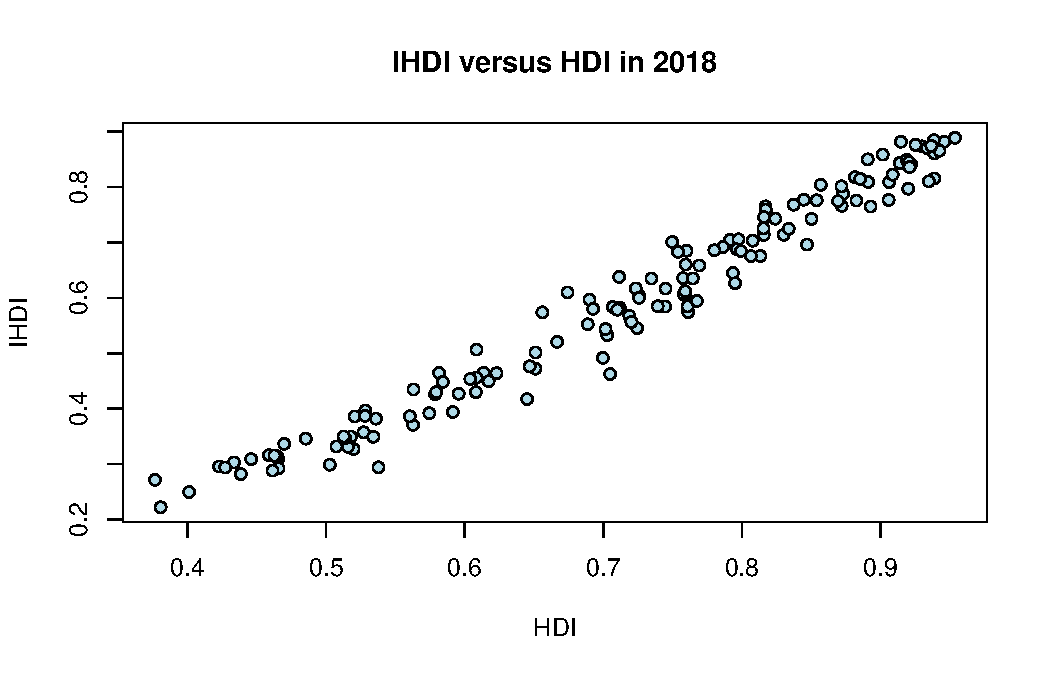
\includegraphics[width=0.9\linewidth]{week8/week8-hdi1-1} 

\end{knitrout}
\end{center}

We want to see if the real per capita GDP is a good measure of
welfare. The following is the scatter plot of IHDI as a function of
GNI. On the left graph, GNI is expressed in thousands of constant
international dollars and on the right graph GNI is expressed in
logs. The red dashed lines have been added to show the overall
comovement between the two variables. Clearly, both graphs show that
there is a strong comovement between GNI and the human development
index. However, there is some variations: we see IHDI gaps being above
0.3 for some countries with the same real per capita GNI. But, the
variation decreases as GNI increases: we see little variation for
countries with log GNI above 10. 

The right graph was added to show you that the observed relationship
is linear on average when GNI is expressed in logs. It means that a
1\% increase in GNI implies a constant increase in IHDI on average (on
the graph below each 1\% increase of GNI is associated with IHDI being
0.0015 higher on average). Since is easier to interpret changes in
percentage rather than changes in constant international dollars, we
will only use that scale for analyze relationships.

\begin{center}
\begin{minipage}{.45\textwidth}  
\begin{knitrout}\footnotesize
\definecolor{shadecolor}{rgb}{0.969, 0.969, 0.969}\color{fgcolor}
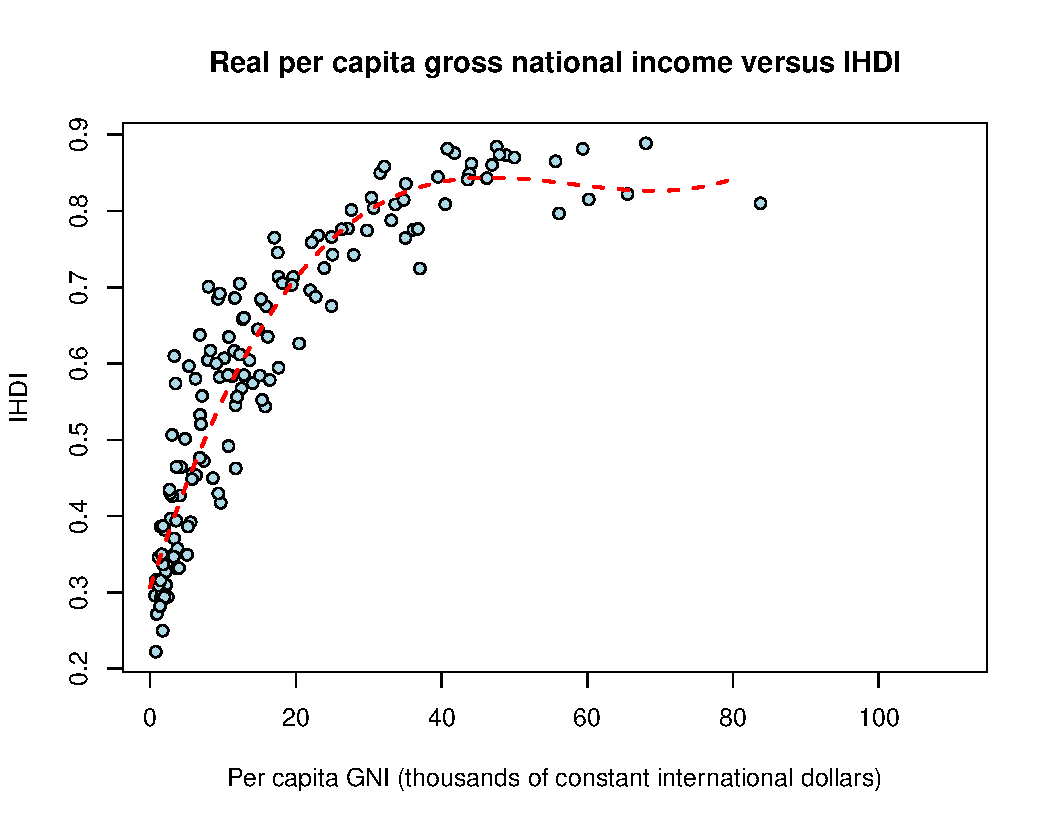
\includegraphics[width=\maxwidth]{week8/week8-hdi2-1} 

\end{knitrout}
\end{minipage}
\begin{minipage}{.45\textwidth}  
\begin{knitrout}\footnotesize
\definecolor{shadecolor}{rgb}{0.969, 0.969, 0.969}\color{fgcolor}
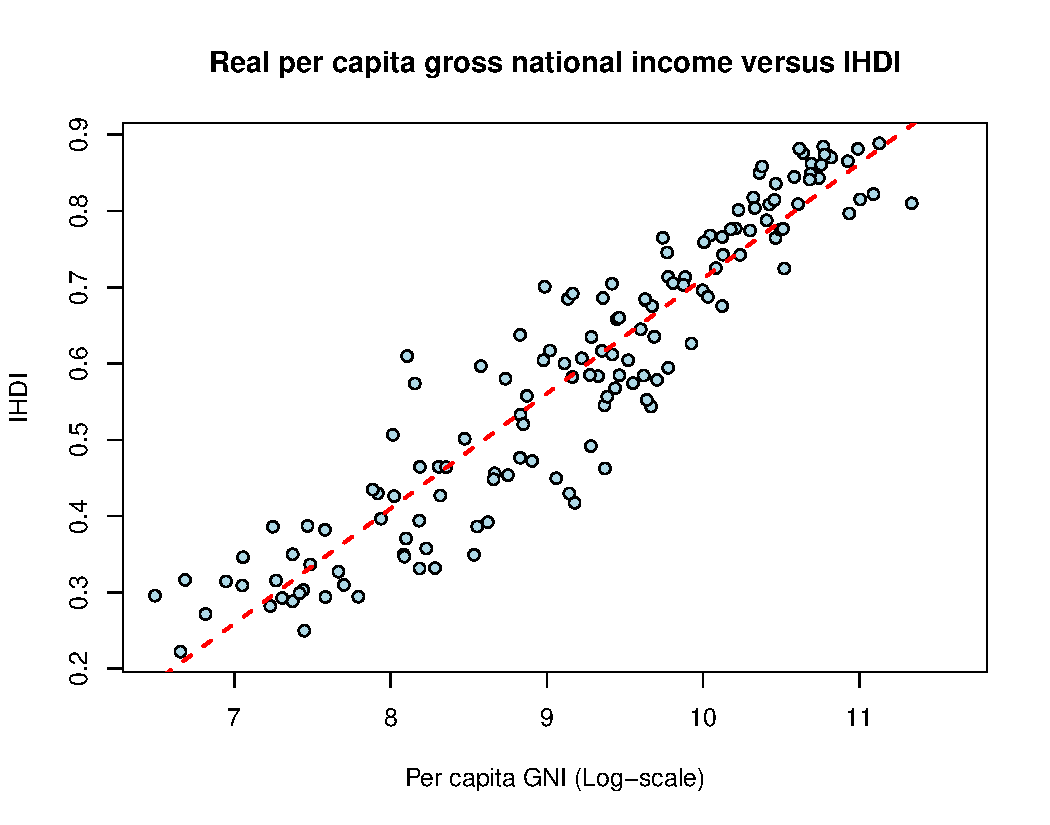
\includegraphics[width=\maxwidth]{week8/week8-hdi3-1} 

\end{knitrout}
\end{minipage}
\end{center}

Next, we want to see if there is a positive comovement between per
capita income and other determinants of welfare. The following graphs
are the scatter plots of life expectancy (left graph) and education
(right graph) with respect to the log of real per capita GNI. Again,
there is a strong positive comovement between real per capita income
and the two variables. However, we also see lots of variations. For
example, the expectancy for Lesotho (LSO) and Honduras (HND) are
respectively 54 and 75 years despite the fact that they have similar
real per capita income. We see the same gap between relatively richer
countries such as Lebanon (LBN) and the Kingdom of Eswatini (SWZ). The
same type of variations is observed is we use the expected level of
education as welfare component (compare South Sudan (SDN) with Togo
(TGO) or the Equatorial Guinea (GNQ) with Argentina (ARG)).

\begin{center}
\begin{minipage}{.45\textwidth}  
\begin{knitrout}\footnotesize
\definecolor{shadecolor}{rgb}{0.969, 0.969, 0.969}\color{fgcolor}
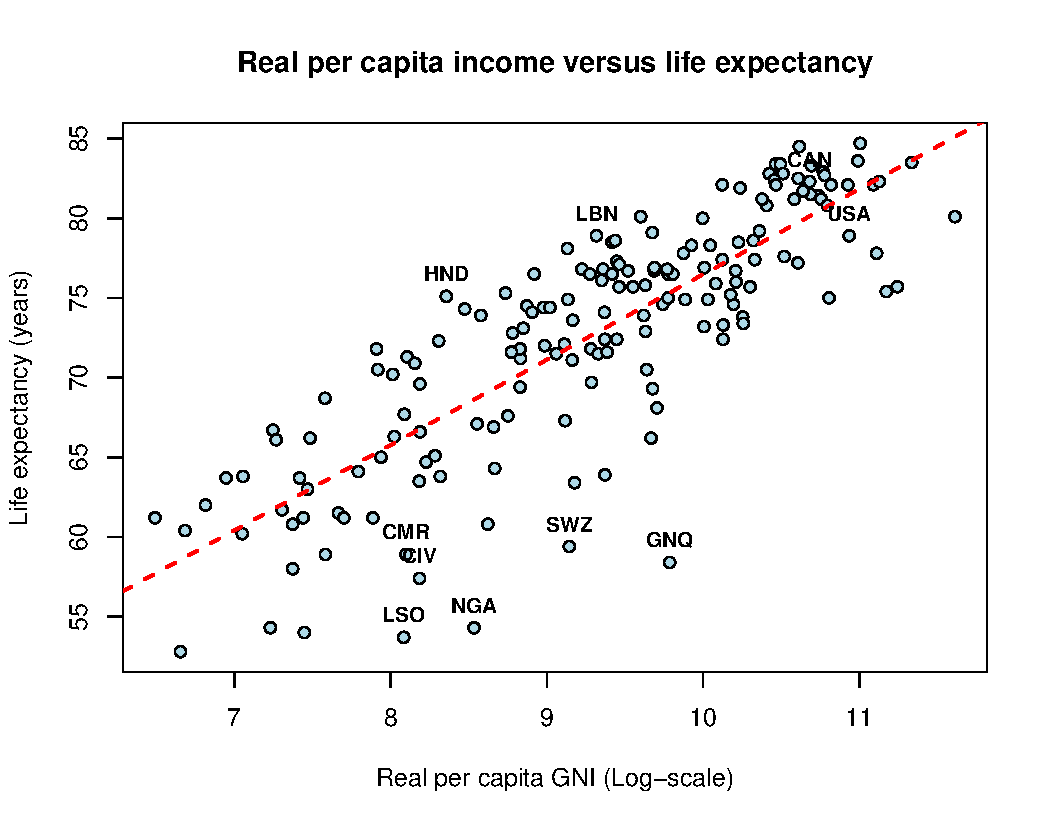
\includegraphics[width=\maxwidth]{week8/week8-hdi4-1} 

\end{knitrout}
\end{minipage}
\begin{minipage}{.45\textwidth}  
\begin{knitrout}\footnotesize
\definecolor{shadecolor}{rgb}{0.969, 0.969, 0.969}\color{fgcolor}
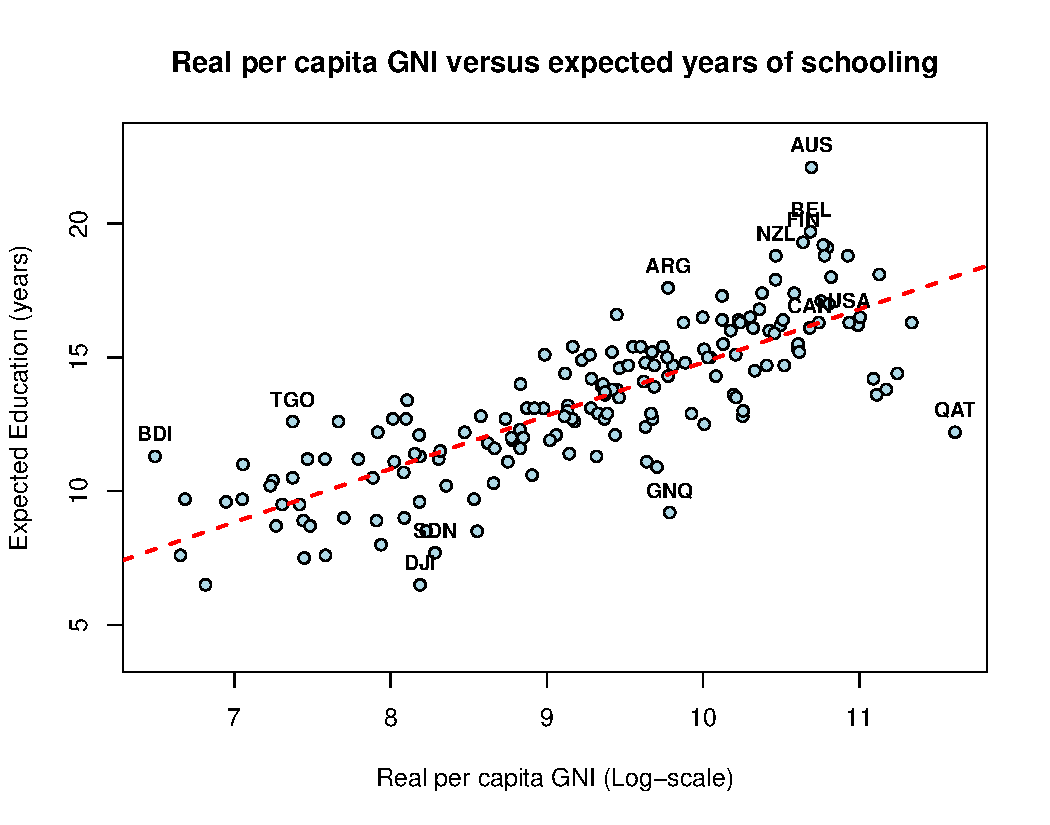
\includegraphics[width=\maxwidth]{week8/week8-hdi5-1} 

\end{knitrout}
\end{minipage}
\end{center}

\subsubsection*{Concluding Remark}

For the rest of the chapter, we will use real per capita GDP as an
indicator of welfare. We are not by any mean pretending that real per
capita GDP is a good measure of welfare. All we say is that it is a
relatively good indicator because it is positively related to most
components that determine welfare (education, health, reduced
inequality, clean water and air, gender equality, peace and justice,
etc.). We just have to keep in mind that higher real per capita GDP
does not necessary imply welfare improvement: we just saw examples of
richer countries with poor human conditions. What we do observe is
that welfare tends to improve eventually as real per capita income
increases.

\subsection{Inequality Across Countries}

The data used in this section are from the Penn World Table (PWT)
version 9.1 \citep{pwt91}. The table is a collection of annual time
series from 1950 to 2017 for 182 countries. Estimating macroeconomic
indicators that can be compared across countries is a difficult tasks
which explains why there are so many versions. Values in version 9.1
may also differ from order data sources such as the World Bank or the
OECD web site. It is an issue for empirical macroeconomists trying to
perform sophisticated statistical studies, but it has little impact on
our graphical analysis. The PWT is useful because it contains longer
time series than the World Bank or the OECD. However, the series are
not complete for all countries. For example, the real GDP is available
for only 30\% of the 182 countries in 1950, 61\% in 1960 and 86\% in
1970. 

\subsubsection*{Income Inequality}


As we saw in previous chapter,  total income is not allocated equally
across countries. We start this section by reassessing this fact using
world data. The following is the histogram of real per capita GDP in
2017 for 182 countries (you can construct the series using the files
PWT91pop.csv and PWT91rgdp.csv). We can see a large proportion of the
countries at the bottom of the income distribution. In fact, more than
half of the countries (98 out of
182) are represented by the first three bars,
implying a per capita real GDP less than 15 thousand (the base of each
rectangle is 5).  The three richest countries at the right of the
histogram are Luxembourg (99.5 thousand), Macao
(97 thousand) and Qatar (100.1 thousand).

\begin{center}
\begin{knitrout}\footnotesize
\definecolor{shadecolor}{rgb}{0.969, 0.969, 0.969}\color{fgcolor}
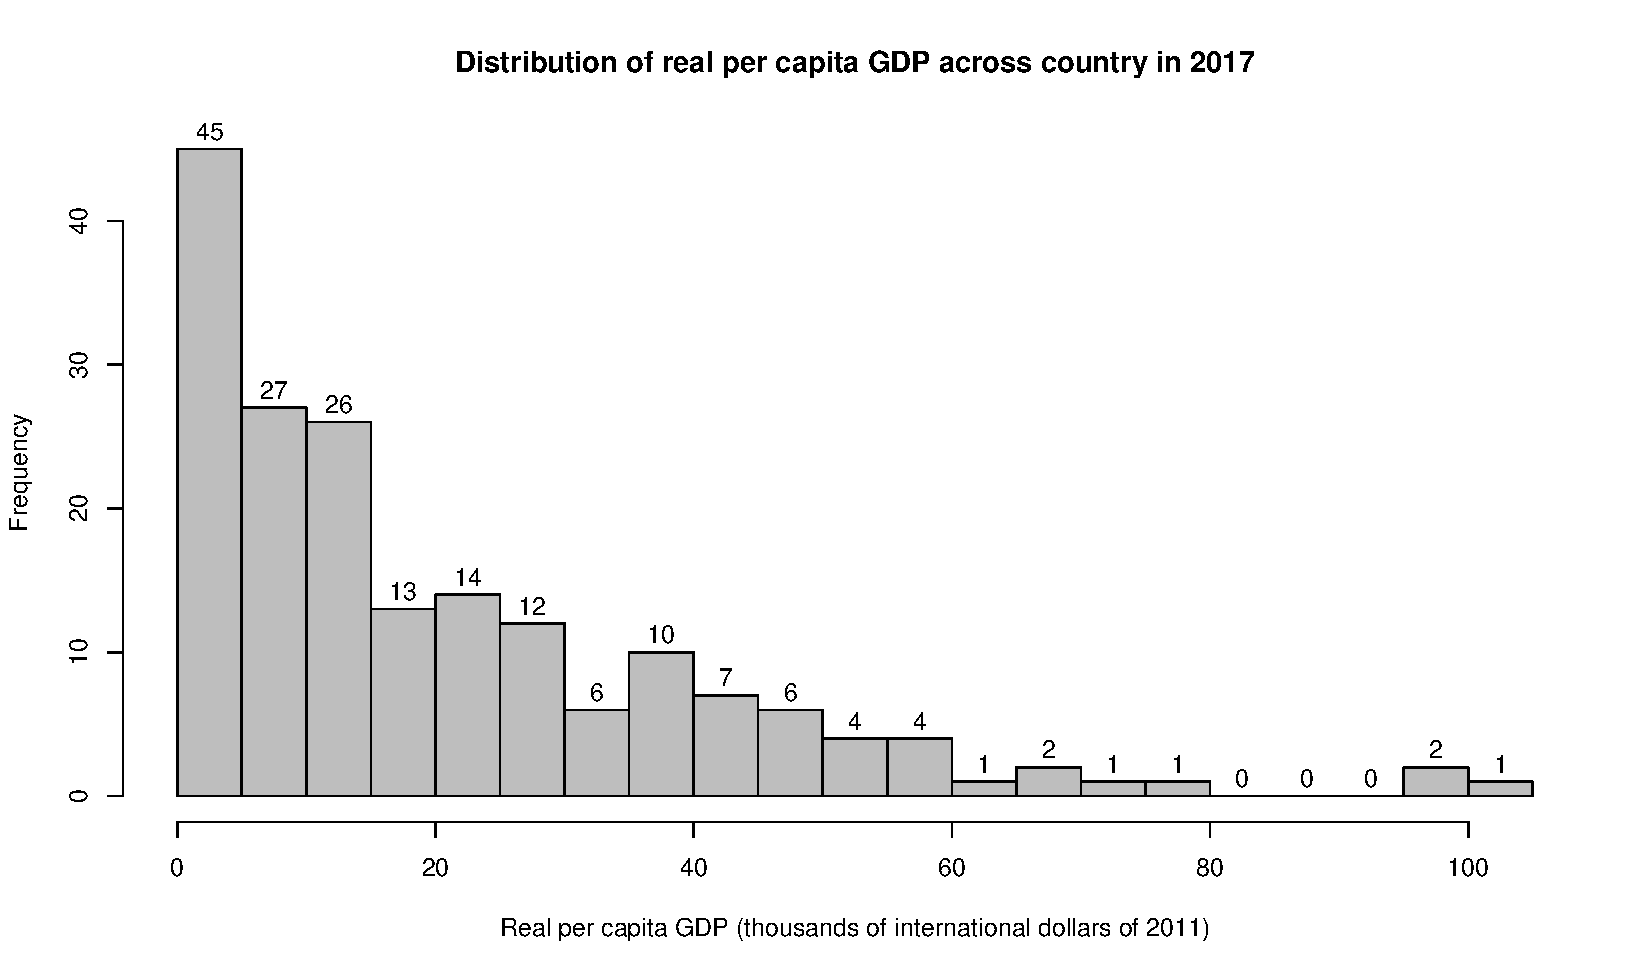
\includegraphics[width=0.7\linewidth]{week8/week8-dist1-1} 

\end{knitrout}
\end{center}



\subsubsection*{Distribution Using Smooth Density}

When we want to compare income distributions over time, it is better
to use smooth density because line charts are easier to interpret than
bar charts when multiple series are represented. A smooth density is
simply a smooth line that covers the bars of the histogram (it is more
complicated than that, but it is good enough for this course). On the
following histogram, the smooth density is represented by the red
dashed line. You can see that the number of rectangles is much higher
than in the previous graphs, because a smooth density is obtained by
increasing the number of intervals. For this course, you don't need to
know more about densities and you don't need to know how to create
them. What you need to know is how to interpret them, which is
identical to interpreting histograms.

\begin{center}
\begin{knitrout}\footnotesize
\definecolor{shadecolor}{rgb}{0.969, 0.969, 0.969}\color{fgcolor}
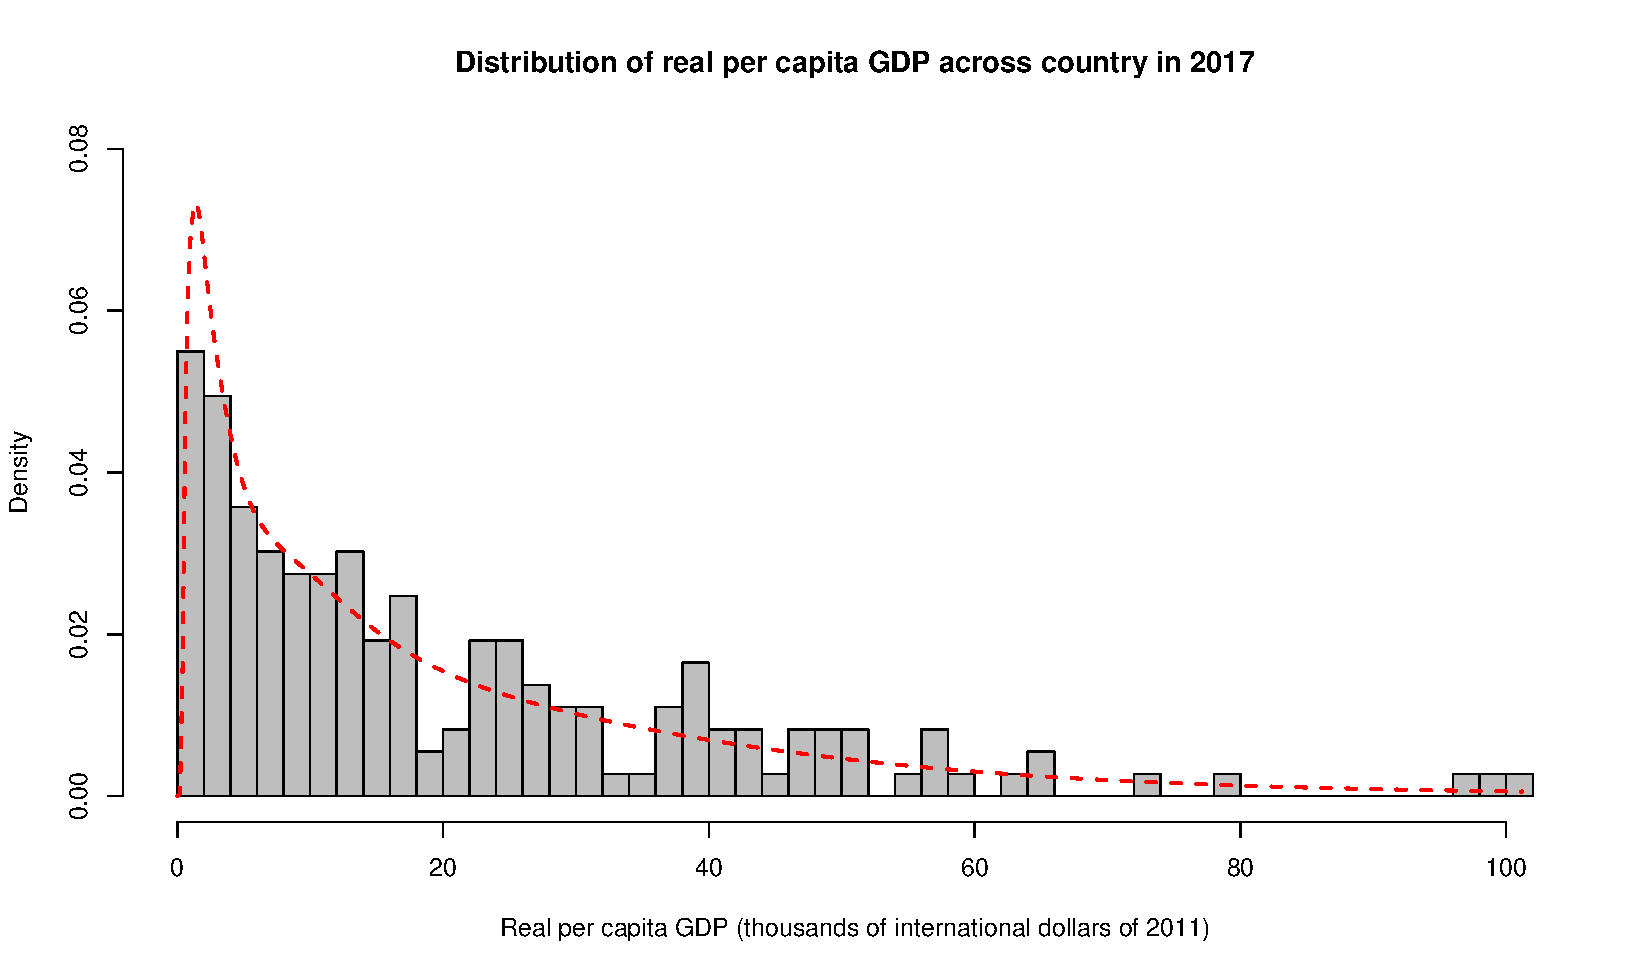
\includegraphics[width=0.7\linewidth]{week8/week8-dist3-1} 

\end{knitrout}
\end{center}

\subsubsection*{The Evolution of the Income Distribution Across Countries}

The distributions for 1960, 1980, 2000 and
2017 are represented respectively by the solid black, the red dashed,
the green dotted and the dot-dashed blue lines. Since the areas under
the curves are proportions, we see that the proportion of poor
countries has decreased during the periods 1960-1980, 1980-2000 and
2000-2017. Also, the growing density in the middle shows that the
proportion of rich (around 40) and medium income (around 20) countries
have increased over the period. Therefore, real per capita GDP has
grown at different rates for different countries and some countries
that were poor in the '60s are still poor today. As a result, we
observe more inequality today than in the '60s. One of the purpose of
economic growth is to explain this change in the income distribution.



\begin{center}
\begin{knitrout}\footnotesize
\definecolor{shadecolor}{rgb}{0.969, 0.969, 0.969}\color{fgcolor}
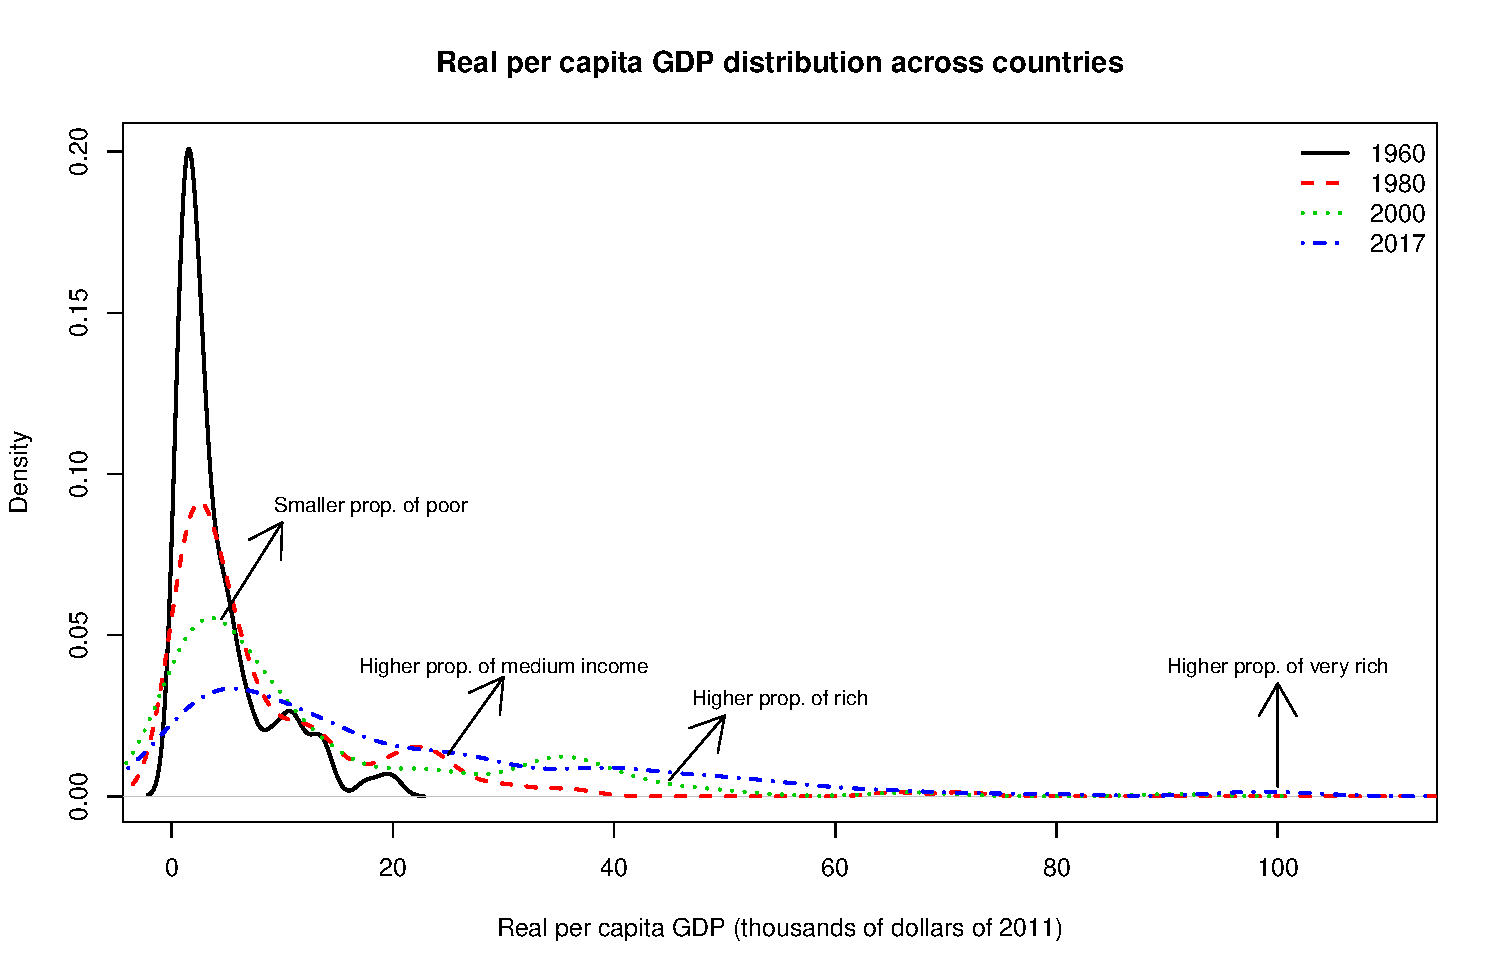
\includegraphics[width=0.7\linewidth]{week8/week8-dist4-1} 

\end{knitrout}
\end{center}

\subsubsection*{Alternative Representation: Log Per Capita GDP Distribution}

In the assigned readings, the author looks at the distribution of real
per capita GDP expressed in logs. The following is what the author
presents with the year 2017 added. You may see small differences
because our graph is based an a different PWT version and also because
the methods for generating the smooth densities may differ from mine.
The distribution for 1960, 1980, 2000 and 2017 are represented
respectively by the solid black, the red dashed, the green dotted and
the dot-dashed blue lines.
\begin{center}
\begin{knitrout}\footnotesize
\definecolor{shadecolor}{rgb}{0.969, 0.969, 0.969}\color{fgcolor}
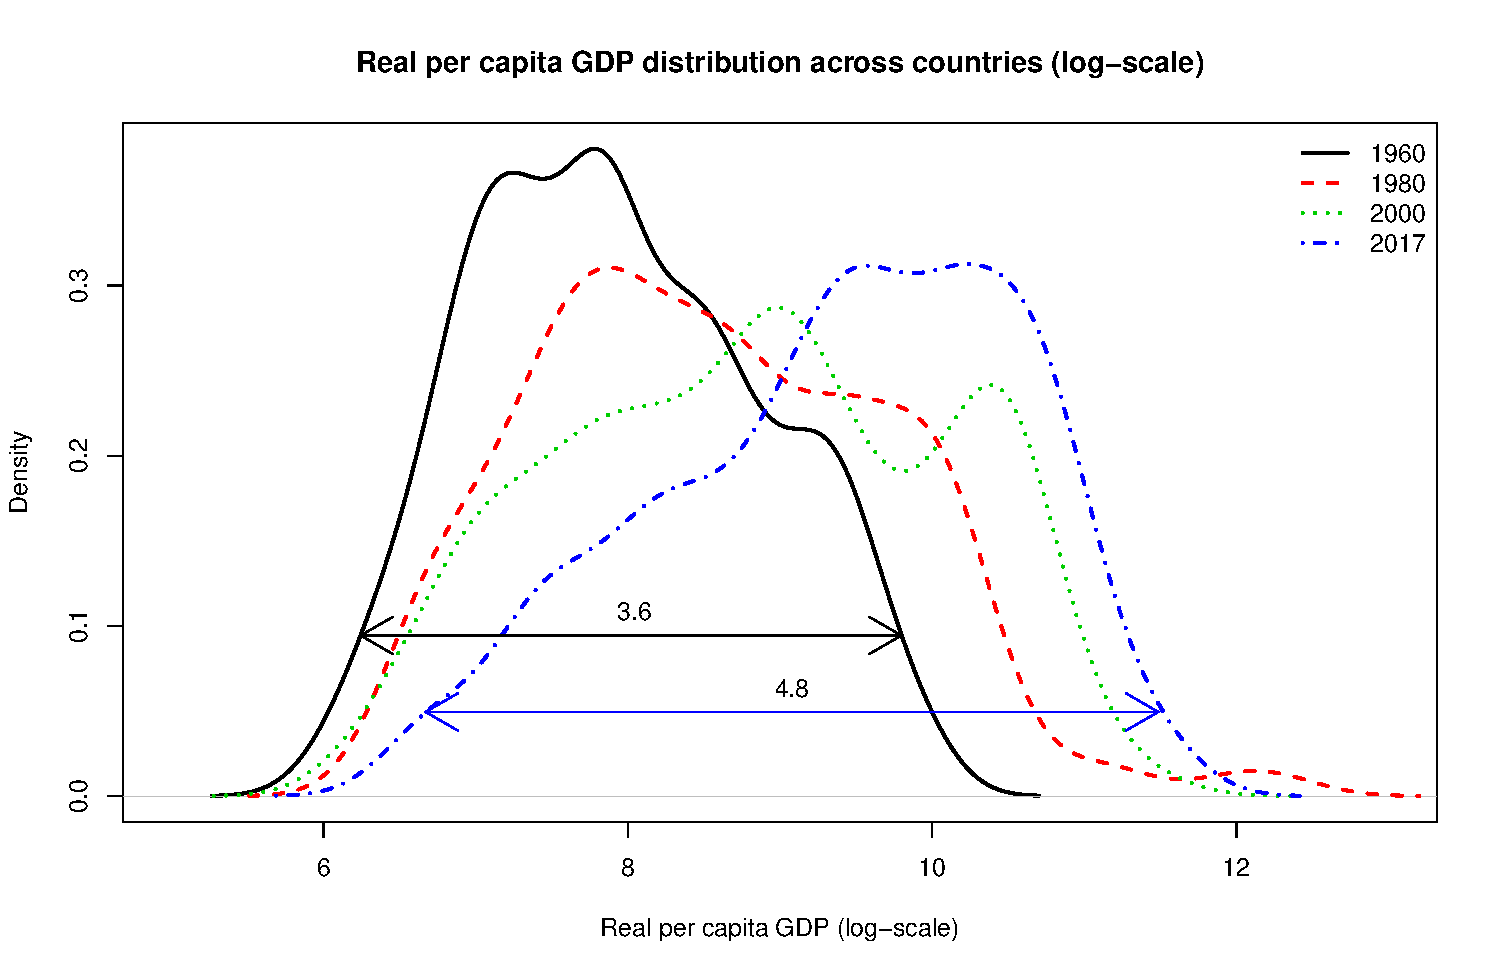
\includegraphics[width=0.7\linewidth]{week8/week8-dist5-1} 

\end{knitrout}
\end{center}
We can see that the distribution is not as skewed as the previous
one. However, we still observe that the gap between poor and rich
countries have increased between 1960 and 2017. The arrows show the
gaps between the first and last percentiles of the distribution in
1960 and 2017. The numbers look similar but they hide huge gaps. In
1960, the gap in log is 3.6, which means:
\begin{eqnarray*}
\log\left(\frac{X_{99}}{X_1}\right) &=& 3.6\\ 
\frac{X_{99}}{X_1} &=& e^{3.6} = 36.6\,,
\end{eqnarray*}
where $X_1$ and $X_{99}$ are the first and 99$^\mathrm{th}$
percentiles. It means that the per capita income of the
99$^\mathrm{th}$ percentile is 36.6 times higher
then the per capita income of the first percentile. In 2017, the per
capita income of the 99$^\mathrm{th}$ percentile is
121.5 higher:
\begin{eqnarray*}
\log\left(\frac{X_{99}}{X_1}\right) &=&  4.8\\ 
\frac{X_{99}}{X_1} &=& e^{4.8} =  121.5\,.
\end{eqnarray*}
Therefore, the shape of the distributions in dollars versus in logs
are different because large differences in dollars translates into
small differences in logs. This is why the the distribution looks more
equally spread on both sides of the center when the variable is
expressed in logs.



To understand why the distribution of the log is less skewed, the
following shows the distribution of real per capita GDP expressed in
thousands of dollars for 2011. On the graph, the red dash line
represents the median, and the dotted blue and dot-dashed green lines
are respectively the per capital incomes of the first and
99$^\mathrm{th}$ percentiles. From the numbers on top of the arrows,
we see that the average per capita income of the 99$^\mathrm{th}$
percentile is 84.1 thousand dollars higher than the
median and it is 12.5 thousand dollars lower for
the first percentile. This is a common characteristic for all skewed
distributions (longer right tail). In proportion, however, the gap is
reversed (numbers under the arrows). The median is 1589.3\%
higher than the first percentile and the 99$^\mathrm{th}$ percentile
is 631.8\% higher than the median.
\begin{center}
\begin{knitrout}\footnotesize
\definecolor{shadecolor}{rgb}{0.969, 0.969, 0.969}\color{fgcolor}
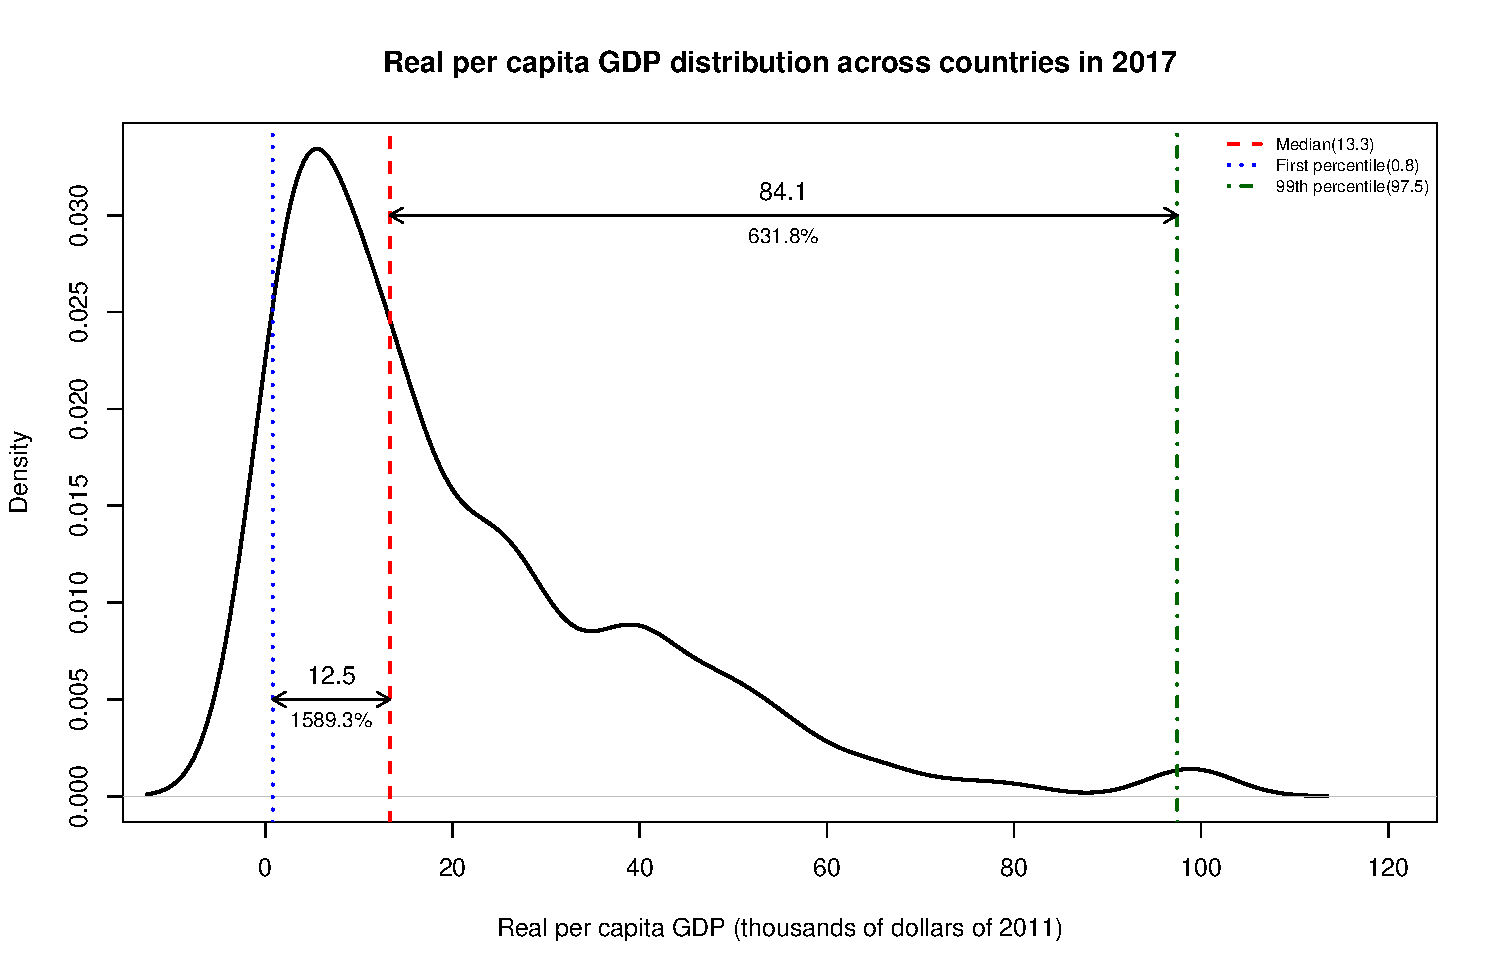
\includegraphics[width=0.7\linewidth]{week8/week8-dist6-1} 

\end{knitrout}
\end{center}
The difference in proportion is what we measure when we use the log
scale. The following graph is the distribution using the log scale. As
for the previous graph, the red dash line represents the median, and
the dotted blue and dot-dashed green lines are the per capital incomes
of the first and 99$^\mathrm{th}$ percentiles.
\begin{center}
\begin{knitrout}\footnotesize
\definecolor{shadecolor}{rgb}{0.969, 0.969, 0.969}\color{fgcolor}
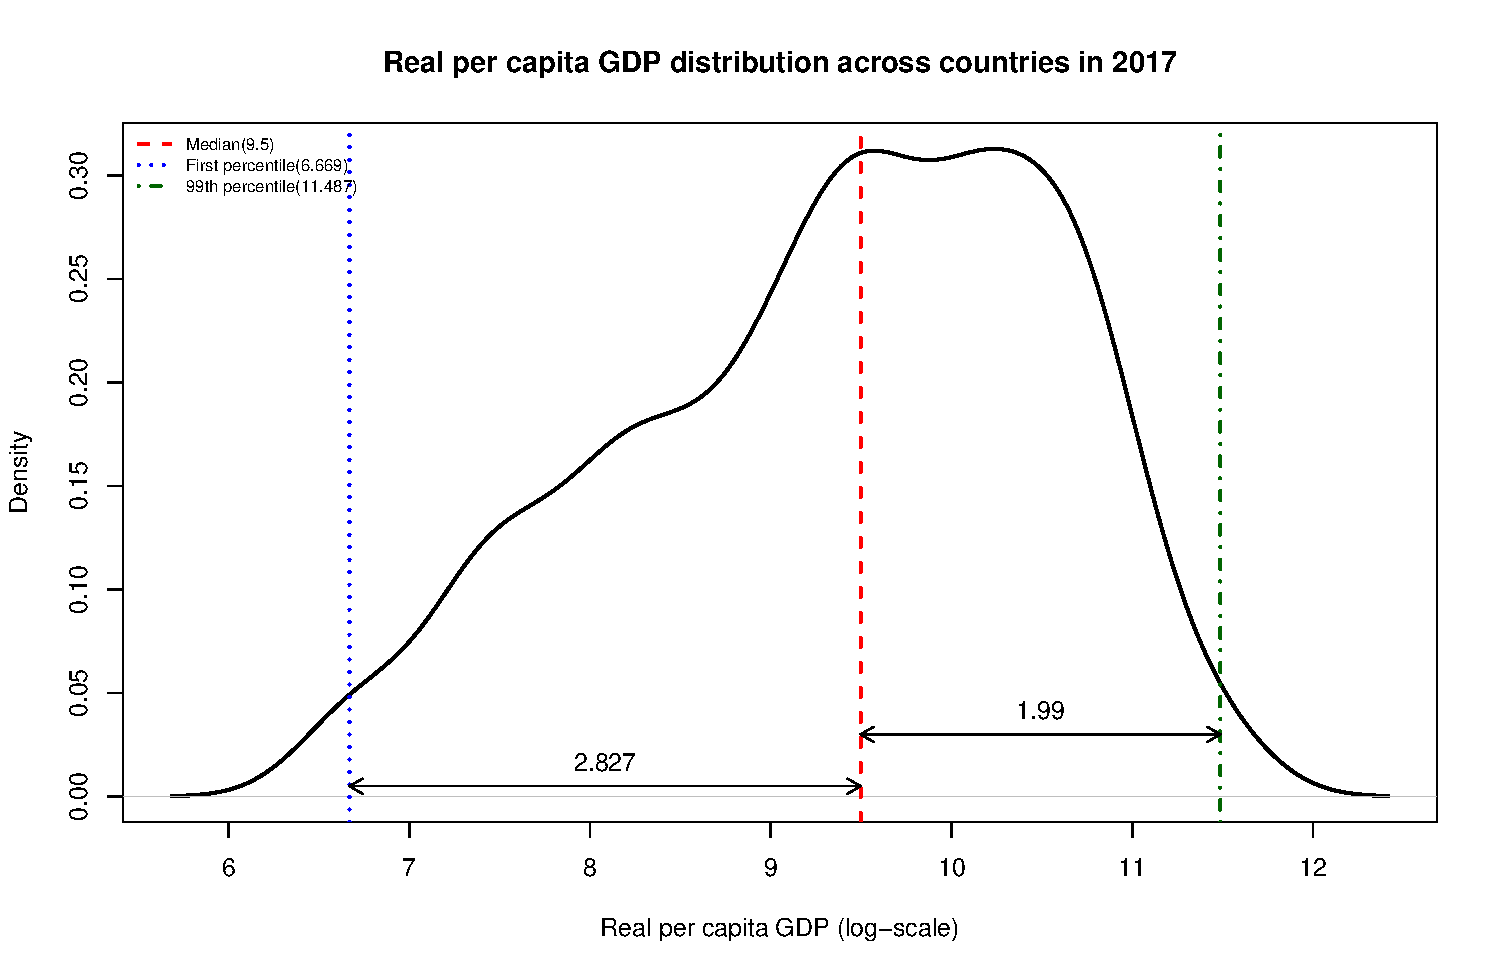
\includegraphics[width=0.7\linewidth]{week8/week8-dist7-1} 

\end{knitrout}
\end{center}
Using the same log formula we obtain approximately the same percentage
differences ($X_m$ is the median and the difference of percentage gaps
are due to rounding errors and how the percentiles are computed in the
two cases):
\begin{eqnarray*}
\log(X_m)-\log(X_1) \equiv \log\left(\frac{X_{m}}{X_1}\right) &=& 2.827\\ 
\frac{X_{m}}{X_1}&=& e^{ 2.827} =  16.8947\\
\frac{X_{m}-X_1}{X_1}\times 100\%  = [16.8947-1]\times 100\%
&=& 1589.47\%
\end{eqnarray*}
and
\begin{eqnarray*}
\log(X_{99})-\log(X_m) \equiv \log\left(\frac{X_{99}}{X_m}\right) &=& 1.99\\ 
\frac{X_{99}}{X_m} &=& e^{ 1.99} =  7.3155\\
\frac{X_{99}-X_m}{X_m}\times 100\%  = [7.3155-1]\times 100\%
&=& 631.55\%\,.
\end{eqnarray*}
Therefore, we need to dig a little deeper to understand distributions
of logs. The most important result to remember is that despite the
fact that the distribution is less skewed, we still observe an
increase in the gap between rich and poor countries.

\subsubsection*{Alternative Representation: Weighed Distribution}

The author also presents the weighted distribution. The problem with
the above method is that it does not take into account that some
countries are much more populated than others. For example, the
population of China in 2017 was 1.4 billion and the population of
Montserrat was 5.2 thousand. Clearly, we cannot consider an increase
of the real per capita GDP in China equivalent to an increase in
Montserrat: the former implies that 1.4 billion individuals are richer
on average while the latter implies only 5.2 thousand richer
individuals on average. Therefore, if we want to visualize the income
distribution in the world at the individual level, we need to increase
the importance of populated countries relative less populated
ones. Learning how to construct a weighted distribution is beyond the
scope of this course but intuitively, it is like constructing a
distribution from a series in which the real per capita GDP of China
is repeated 1.4 billion times, the real per capita GDP of Montserrat is
repeated 5.2 thousand times and so on.



The following graphs reproduces Figure 1.3 of the assigned readings with
the year 2017 added. The distribution for 1960, 1980, 2000 and 2017
are represented respectively by the solid black, the red dashed, the
dotted green and the dot-dashed blue lines. We can see that the per
capita income as increased for a large proportion of the world
population between 1960 and 2017 (large shift of the hill to the
right). This is partly due to the economic growth in China and India,
two countries that represent about 30\% of the world population (real
per capita GDP was multiplied by 10 in China between 1960 and 2017 and
it was multiplied by 4 in India). However, the gap between the poor
and rich has increased even at the individual level (a difference in
logs of 3.5 in 1960 and 4.3 in 2017 between percentiles
1 and 99, not shown on the graph).

\begin{center}
\begin{knitrout}\footnotesize
\definecolor{shadecolor}{rgb}{0.969, 0.969, 0.969}\color{fgcolor}
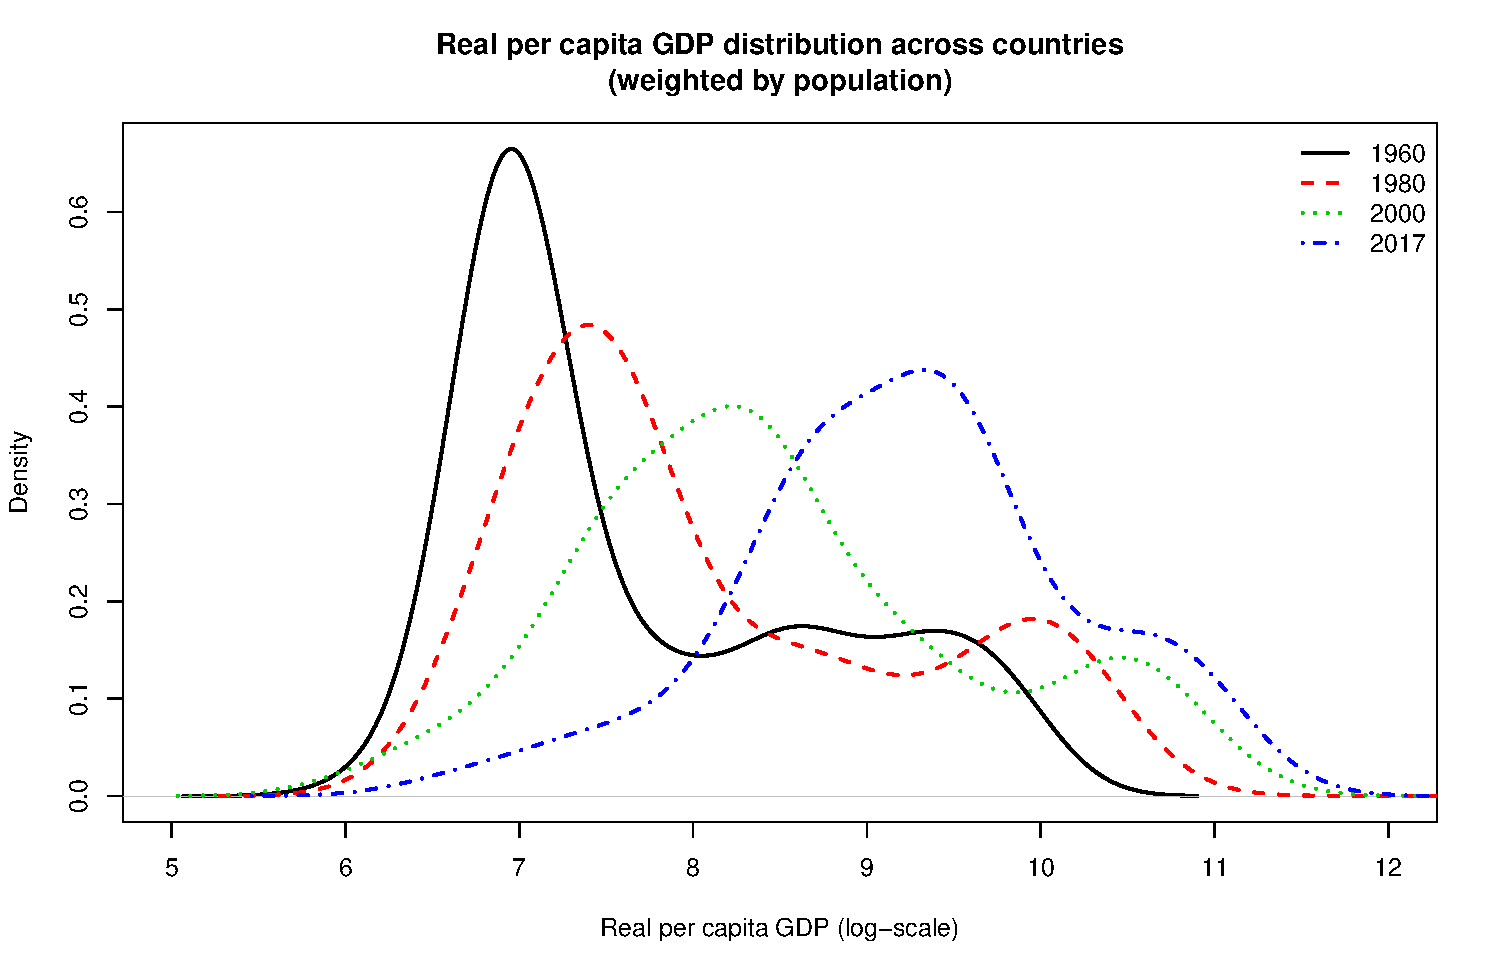
\includegraphics[width=0.7\linewidth]{week8/week8-dist8-1} 

\end{knitrout}
\end{center}


\subsection{The Importance of Growth}

This chapter is called Economic growth (growth rate of the real per
capita GDP) because growth is what allows poor countries to become
richer. In fact, a small difference in the annual growth rate over a
long period of time has a huge impact on the standard of living. To
see that, suppose that the initial real per capita GDP is $X_0$ and
the annual growth rate is $g$ for $T$ years. We saw in a previous
chapter that it implies the following real per capita GDP after $T$
years:
\[
X_T = (1+g)^T X_0\,.
\]
Therefore, the real per capita GDP is multiplied by $(1+g)^T$. For
example, suppose two countries start with the same real per capita
GDP, but the annual growth rate over a period of 50 years in the first
country is 1\% and it is 2\% in the second. Then, the real per capita
GDP is multiplied by
\[
(1+g)^T = (1.01)^{50} = 1.6
\]
in the first country and by 
\[
(1+g)^T = (1.02)^{50} = 2.7
\]
in the second. For example, if $X_0$ was 10 thousand dollars for both
countries, the real per capita GDP after 50 years would become
16 thousand dollars in the first country and
27 thousand in the second. Therefore, the
extra percentage point results in 
11 thousand dollars
more real income by individual on average. 

The following graph compares the trending behaviour of real per capita
GDP for countries with the same initial value but with annual growth
rates ranging from 0.5\% to 3\%, over a period of 70 years (1950 to
2020). On the left graph the GDP is expressed in thousands of dollars
and it is expressed in logs on the right graph. 
\begin{center} 
\begin{minipage}{.45\textwidth}  
\begin{knitrout}\footnotesize
\definecolor{shadecolor}{rgb}{0.969, 0.969, 0.969}\color{fgcolor}
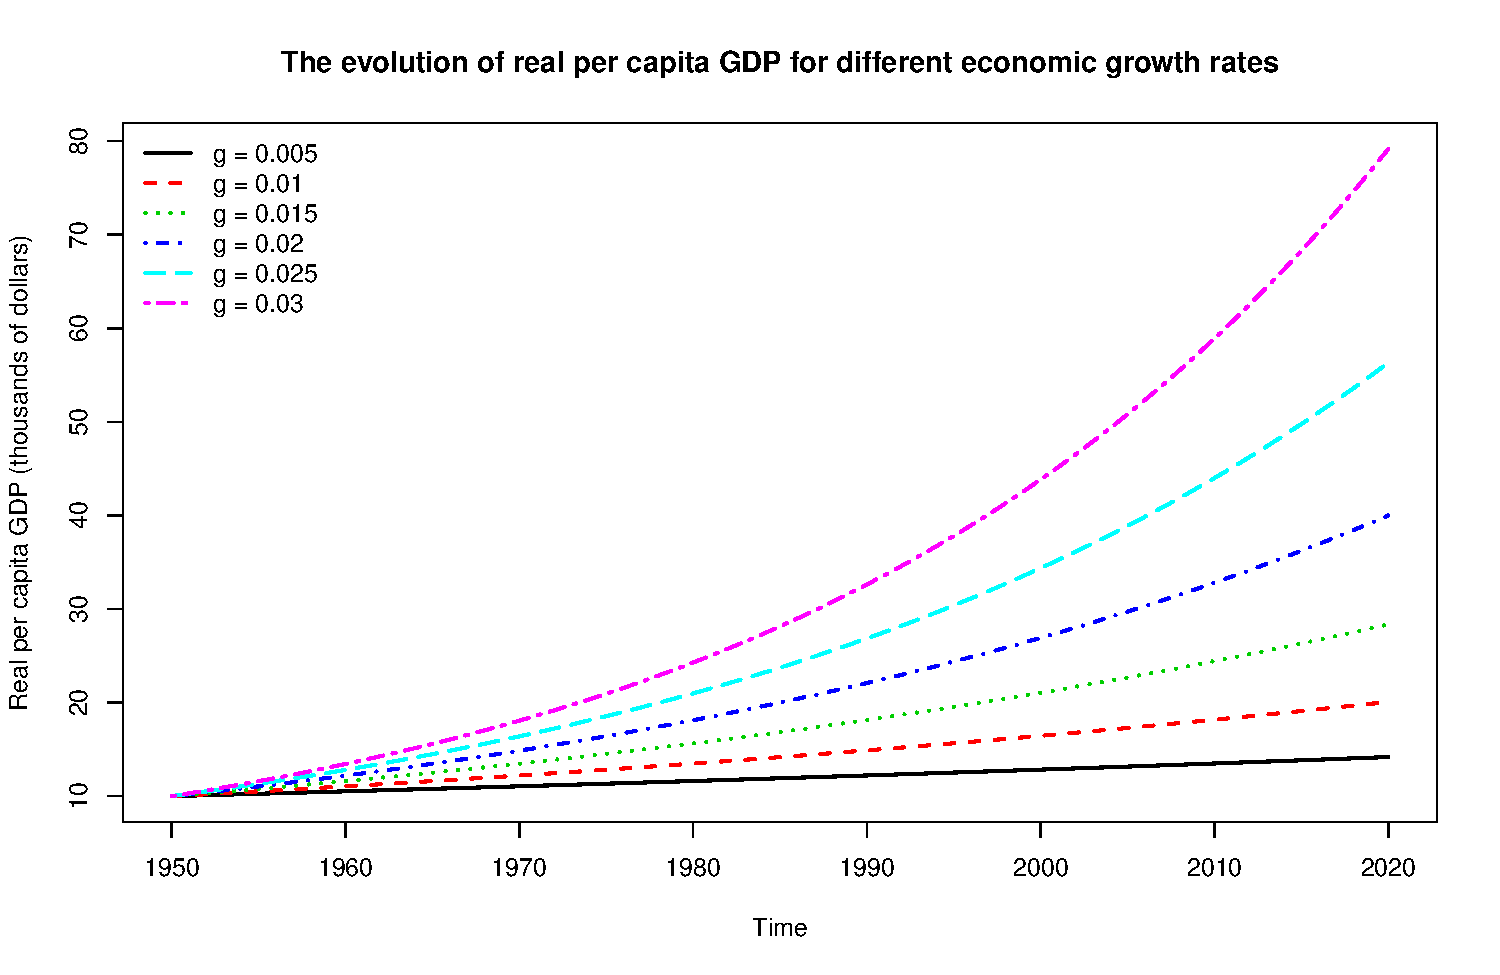
\includegraphics[width=0.9\linewidth]{week8/week8-growth1-1} 

\end{knitrout}
\end{minipage}
\begin{minipage}{.45\textwidth}  
\begin{knitrout}\footnotesize
\definecolor{shadecolor}{rgb}{0.969, 0.969, 0.969}\color{fgcolor}
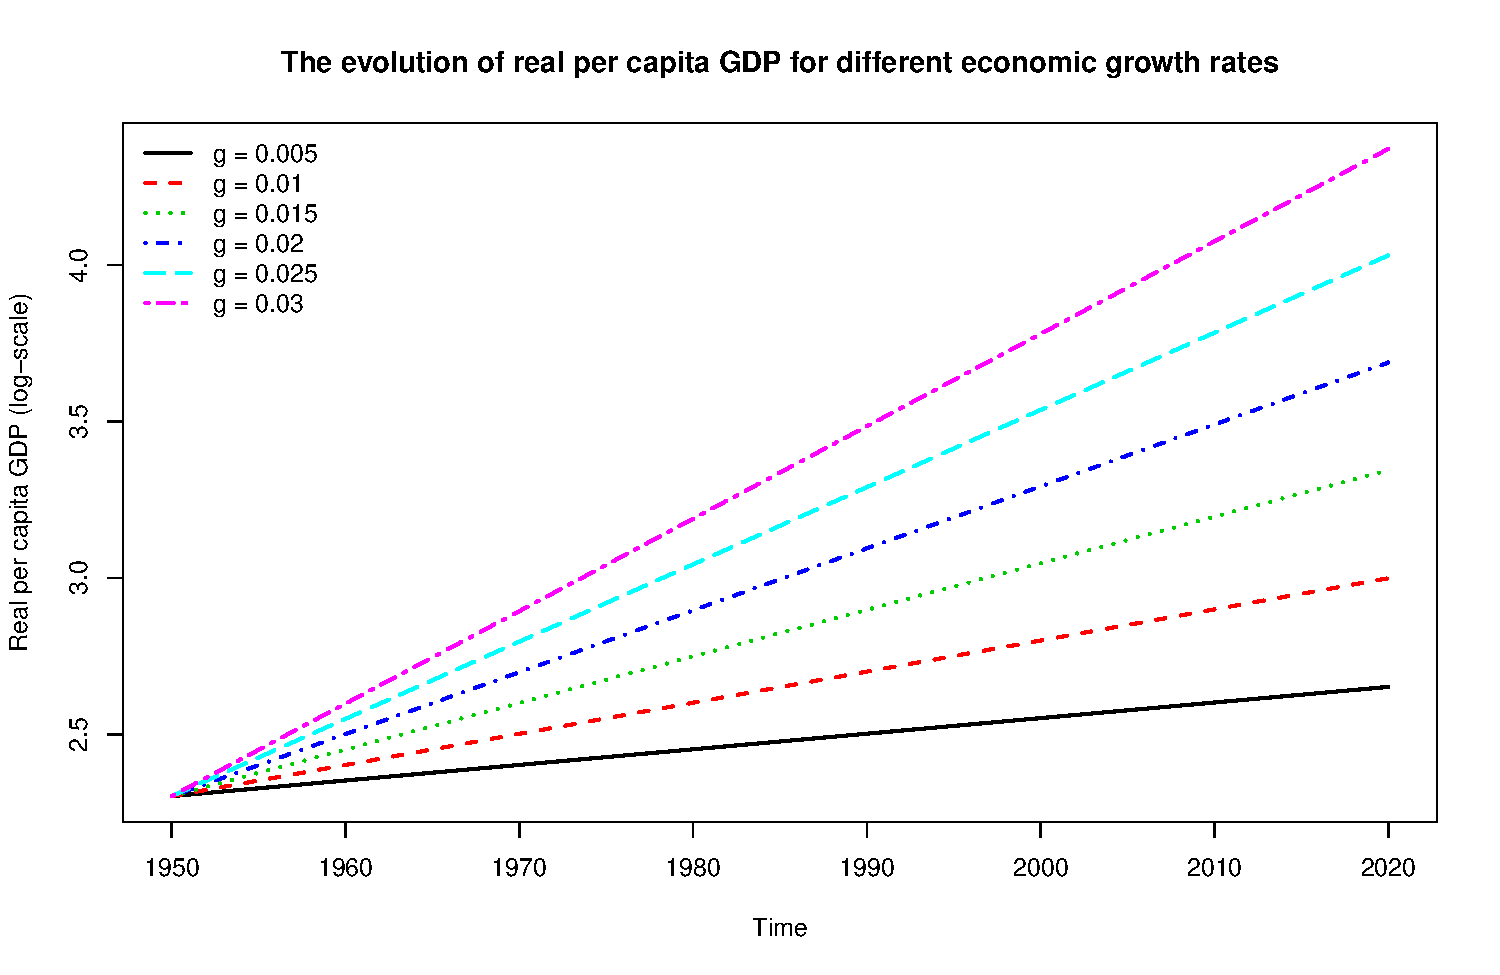
\includegraphics[width=0.9\linewidth]{week8/week8-growth2-1} 

\end{knitrout}
\end{minipage}
\end{center}
We can see that gaps between slow and fast growing economies are
increasing over the period. Therefore, inequality in economic growth
rates leads to income inequality. Notice that the gap in dollars
between consecutive trends in a given year increases as we move up on
the left graph. In other words, the difference of GDP in dollars in
2020 between the countries with $g=0.005$ and $g=0.01$ is smaller than
the difference between the countries with $g=0.025$ and
$g=0.03$. However, the right graph shows that the percentage
differences are the same (same difference in logs implies same
percentage difference).

\subsection{Convergence and Conditional Convergence}

\subsubsection*{The Concept of Convergence}

Some models from the economic growth theory predicts that inequality
across countries (or some countries) should eventually be reduced,
because poor countries should grow faster than rich countries. This
result is called convergence because it implies that the standard of
living of poor and rich countries will eventually converge to the
same. The following graph illustrates the concept of convergence. The
growth rates are the same used in the previous graphs but the 1950
per capita GDP of the faster growing countries are set to a lower
value. Since poor countries grow faster (e.g. the dot-dashed pink
line), they eventually reach the same standard of living as the
countries that were initially rich (e.g. the solid black line).

\begin{center} 
\begin{knitrout}\footnotesize
\definecolor{shadecolor}{rgb}{0.969, 0.969, 0.969}\color{fgcolor}
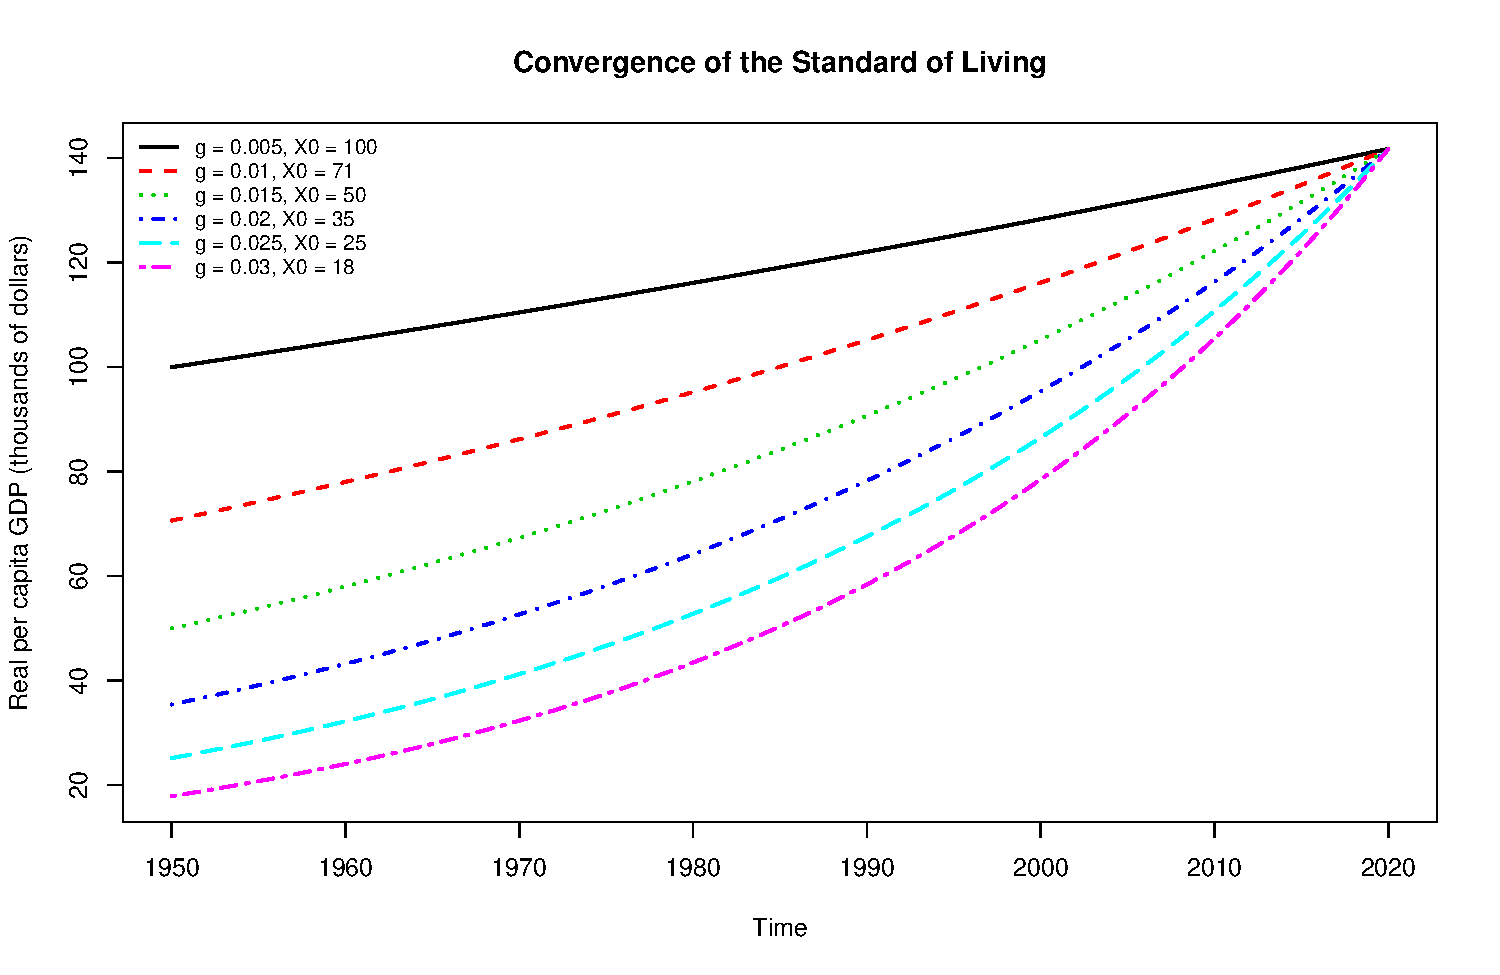
\includegraphics[width=0.7\linewidth]{week8/week8-growth3-1} 

\end{knitrout}
\end{center}

The above graph does not show exactly what convergence means in
theory. If poor countries grow faster than rich countries, then their
growth rates should decrease as they get richer, which is not what we
observe on the graph. In fact, if we continued the lines after 2020,
we would observe a divergence with the poorest country becoming the
richest and the richest becoming the poorest. The purpose of the graph
is just to explain what it means for countries to converge to the same
real per capita GDP. We also want to point out that convergence exists
only if poor countries grow faster than rich countries. The following
graph shows what convergence means: the growth rate is slowing down as
countries get richer. If we were to continue the lines passed 2020, all
lines would get closer and closer from each other. It implies that at
any point in time poorer countries grow faster. That's the only fact
about convergence that we need to understand before going to the next
section.
\begin{center} 
\begin{knitrout}\footnotesize
\definecolor{shadecolor}{rgb}{0.969, 0.969, 0.969}\color{fgcolor}
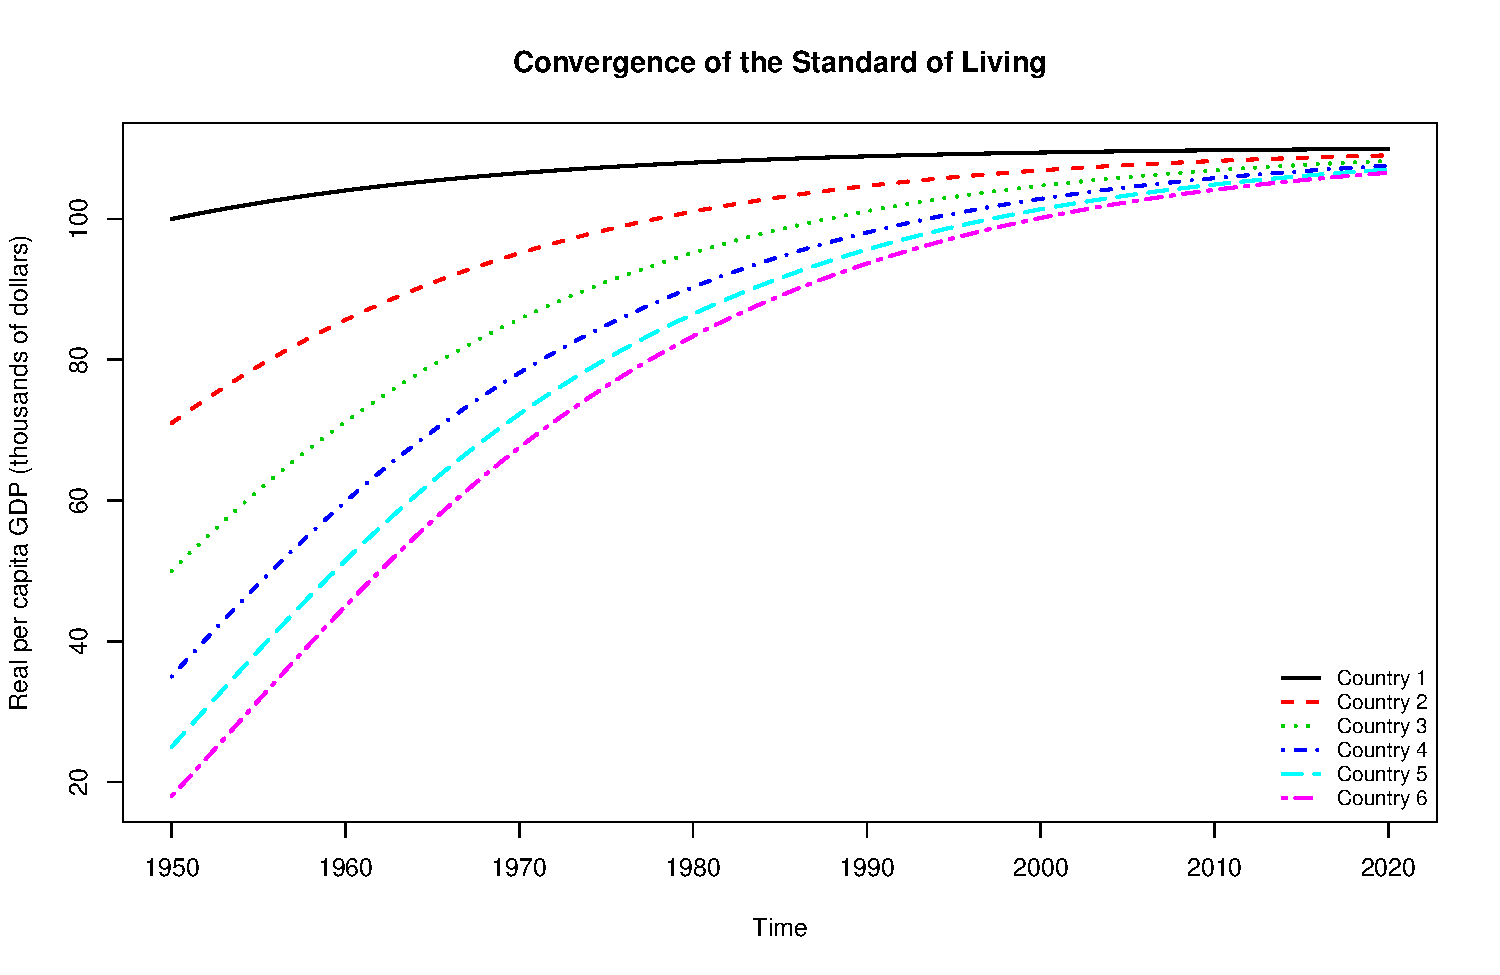
\includegraphics[width=0.7\linewidth]{week8/week8-growth4-1} 

\end{knitrout}
\end{center}

\subsubsection*{Convergence in the Data}


The following graph shows the trend component of the real per capita
GDP expressed in logs for some countries between 1950 and 2017 using a
quadratic trend. In this group of countries, Canada (the solid black
line) was the richest country in 1950 and China (the dotted green
line) was the poorest. The legend includes the average annual growth
rates over the period. We can see that China, Japan (dashed red line)
and India (dot-dashed blue line) are converging to Canada, Nigeria
(log dashed cyan line) is diverging (the gap is increasing) and Mexico
(two-dashed magenta line) is neither converging nor diverging
(constant gap). Therefore, convergence does not seem to be a rule for
all countries.

\begin{center} 
\begin{knitrout}\footnotesize
\definecolor{shadecolor}{rgb}{0.969, 0.969, 0.969}\color{fgcolor}
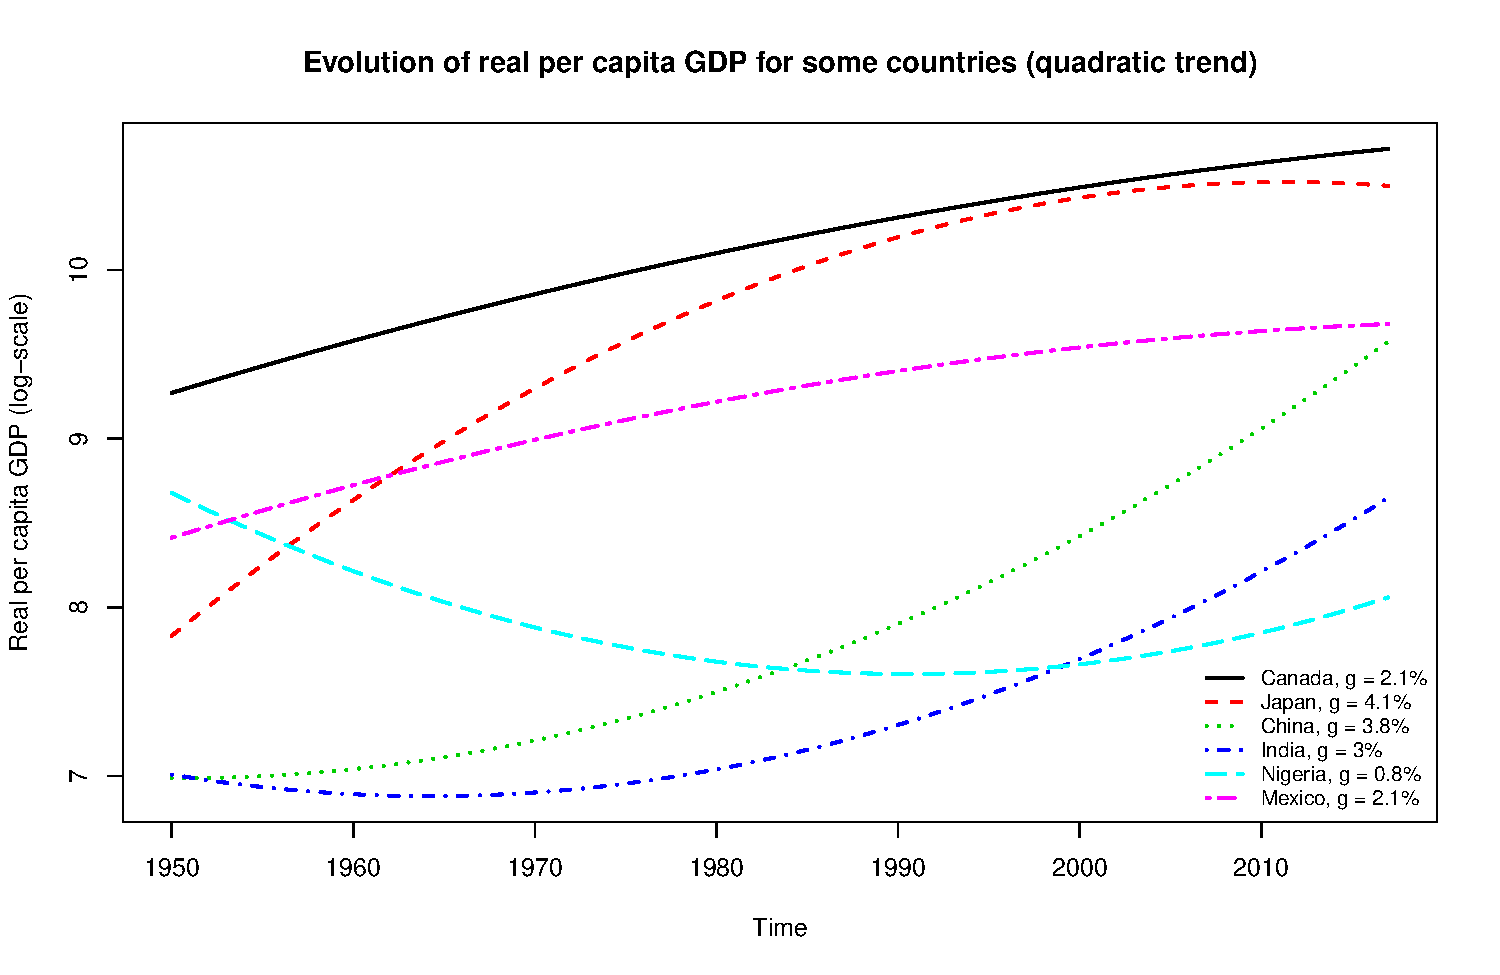
\includegraphics[width=0.7\linewidth]{week8/week8-growth6-1} 

\end{knitrout}
\end{center}





\subsubsection*{Observing Convergence using Scatter Plots}

We can easily verify if there is a global tendency for the poor
countries to grow faster. All we need is a scatter plot of the average
annual growth rate over the whole period with respect to the initial
real per capita GDP. The average growth rate can be computed by
averaging the log differences $(\log(X_t)-\log(X_{t-1}))$ for each
country. A negative comovement between these two variables means that
countries that were initially poor grow faster than countries that
were initially rich, which is what convergence implies. For example,
the following is the scatter plot using the hypothetical series from
the previous section. The graph shows a clear negative comovement
between the two variables: the richest country in 1960 (Country 1) is
the one with the lowest average growth rate between 1960 and 2020 and
the poorest country in 1960 (Country 6) is the one with the highest
average growth rate.
\begin{center} 
\begin{knitrout}\footnotesize
\definecolor{shadecolor}{rgb}{0.969, 0.969, 0.969}\color{fgcolor}
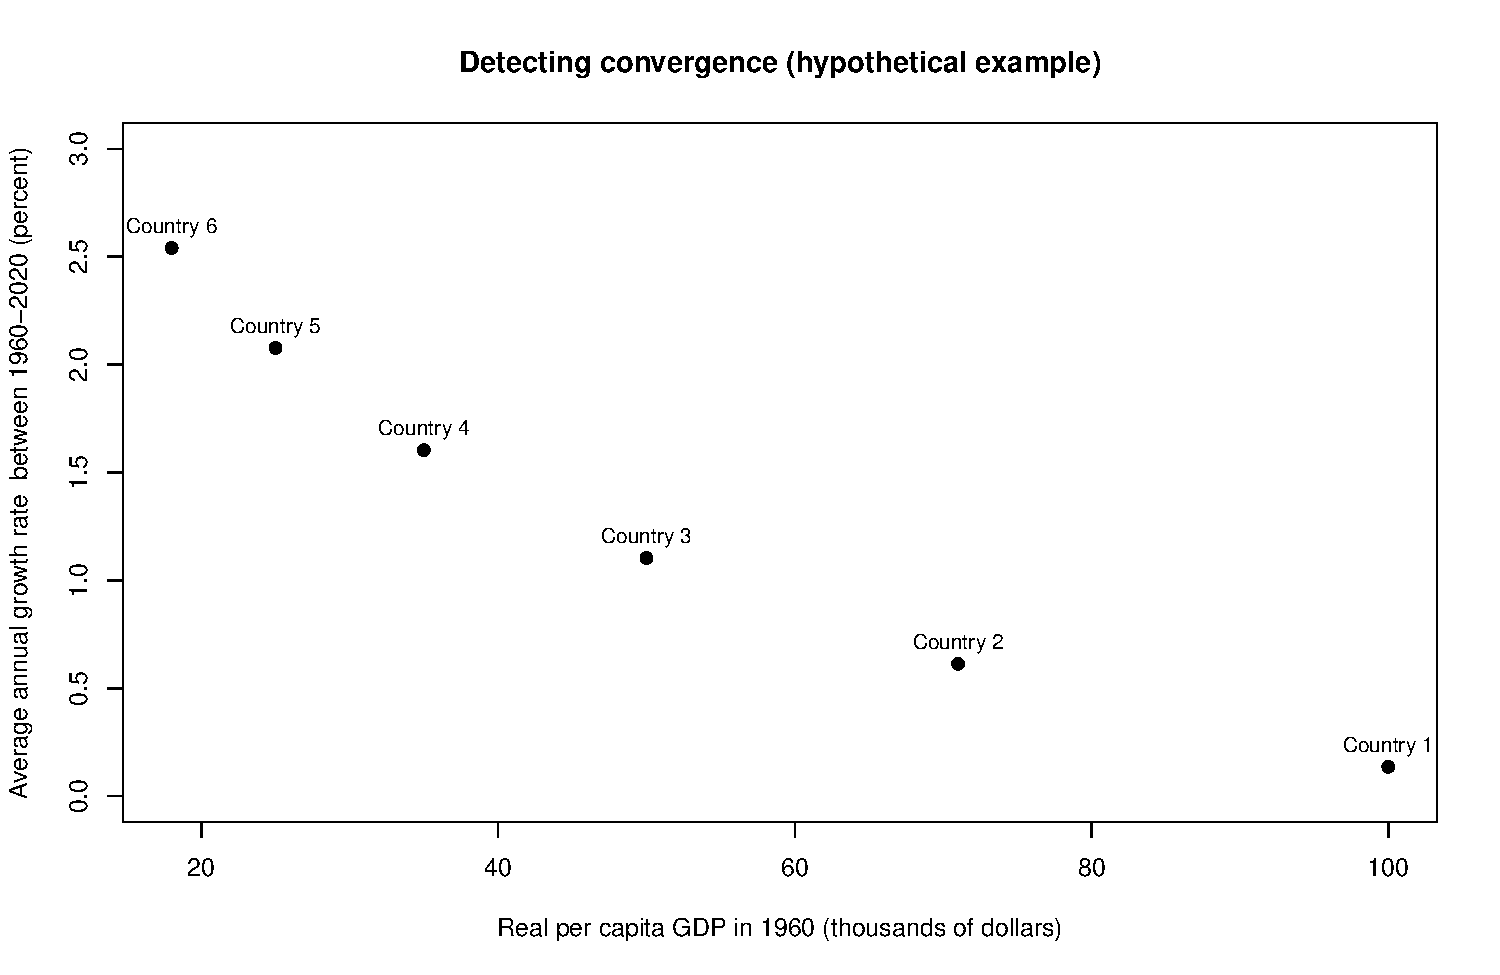
\includegraphics[width=0.7\linewidth]{week8/week8-growth7-1} 

\end{knitrout}
\end{center}



The following is the scatter plot using the 111
countries for which the initial real per capita GDP was available in
1960 and before, using the file Characteristics.csv. On the x-axis, we
have the initial real per capita GDP (the initial year varies from
country to country) and on the y-axis it is the average growth rate
between the year when the first real per capita GDP is available and
2017. The red dashed line is added to show you the
average comovement between the two variables. Clearly, we do not
observe overall convergence: among the initially poorest countries,
the growth rates range between -1.3\% and
6.4\%. For example, the average economic growth
rate for the Democratic Republic of the Congo (COD) from 1950 to
2017 is -1.32\%. It means that its
real per capita GDP was divided by more than 2 during that period
($X_T/X_0=(1-0.0132)^{67}=
0.411$). On the other
extreme, the average growth rate for the Republic of Korea (KOR), an
equally poor country in 1953, is 5.63\%:
its per capita GDP was multiplied by
33.296
($X_T/X_0=(1+0.0563)^{64}=
33.296$) between 1953
and 2017. Therefore, some countries that were initially
poor are converging but others are diverging.

\begin{center} 
\begin{knitrout}\footnotesize
\definecolor{shadecolor}{rgb}{0.969, 0.969, 0.969}\color{fgcolor}
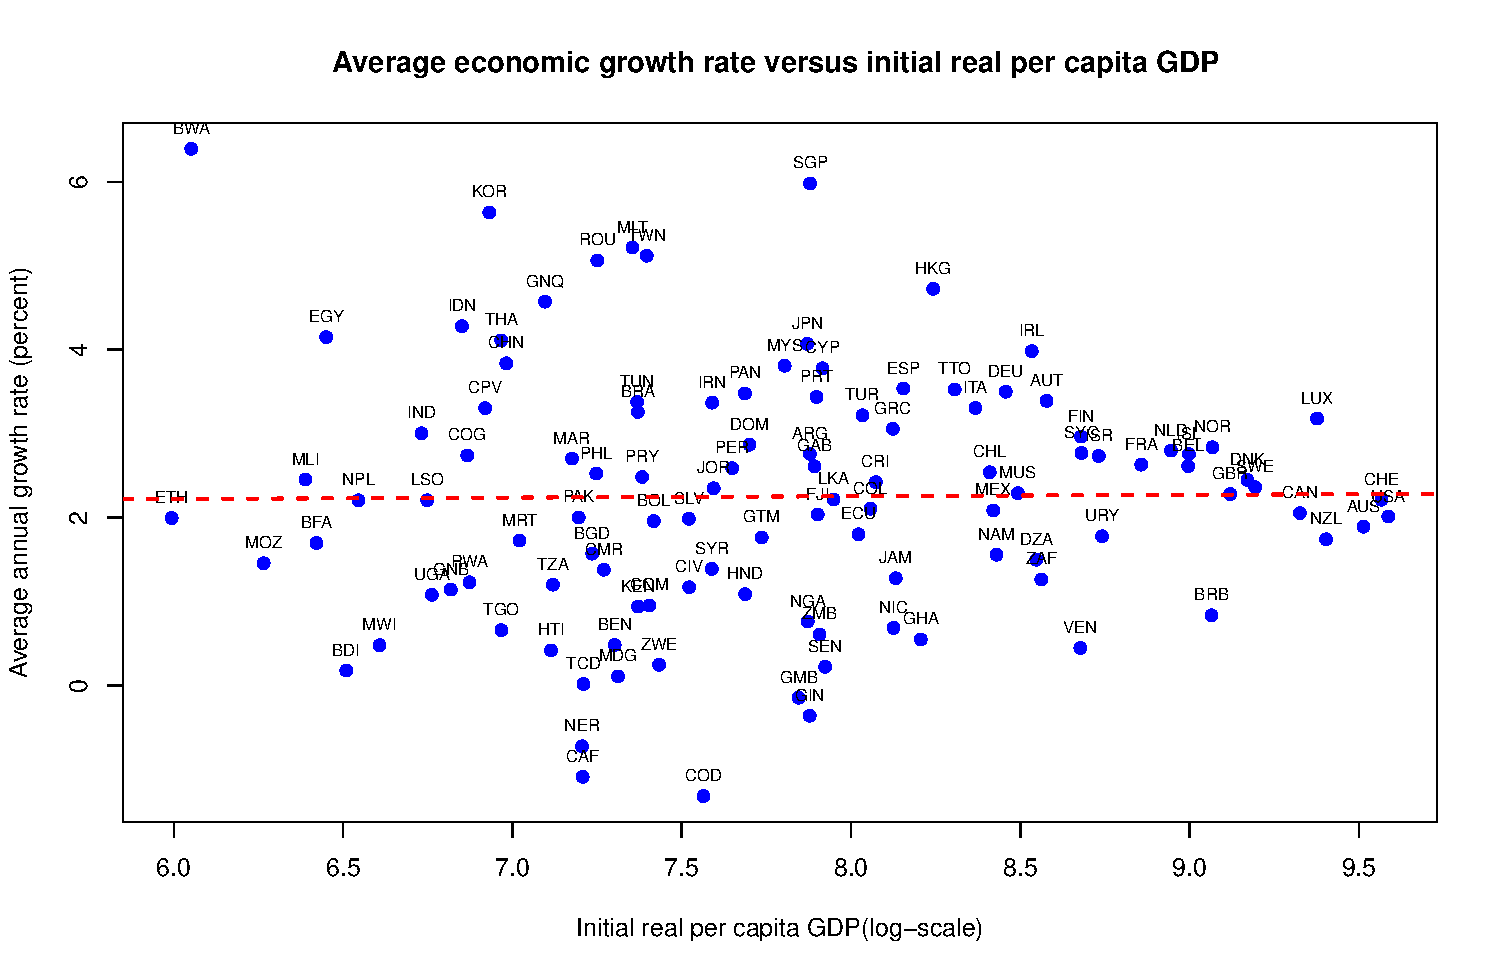
\includegraphics[width=0.7\linewidth]{week8/week8-growth8-1} 

\end{knitrout}
\end{center}

\subsubsection*{Conditional Convergence}

The following graph is the same scatter plot restricted to the
countries that were members of the OECD in 2007 (the choice of 2007 is
arbitrary). We detect a negative comovement between the variables
(look at the red dashed line), which implies that OECD members are
converging to each other on average. We do, however, observe some
variations: Republic of Korea (KOR) and Japan (JPN) are converging
much faster than Mexico (MEX) and Turkey (TUR).
\begin{center} 
\begin{knitrout}\footnotesize
\definecolor{shadecolor}{rgb}{0.969, 0.969, 0.969}\color{fgcolor}
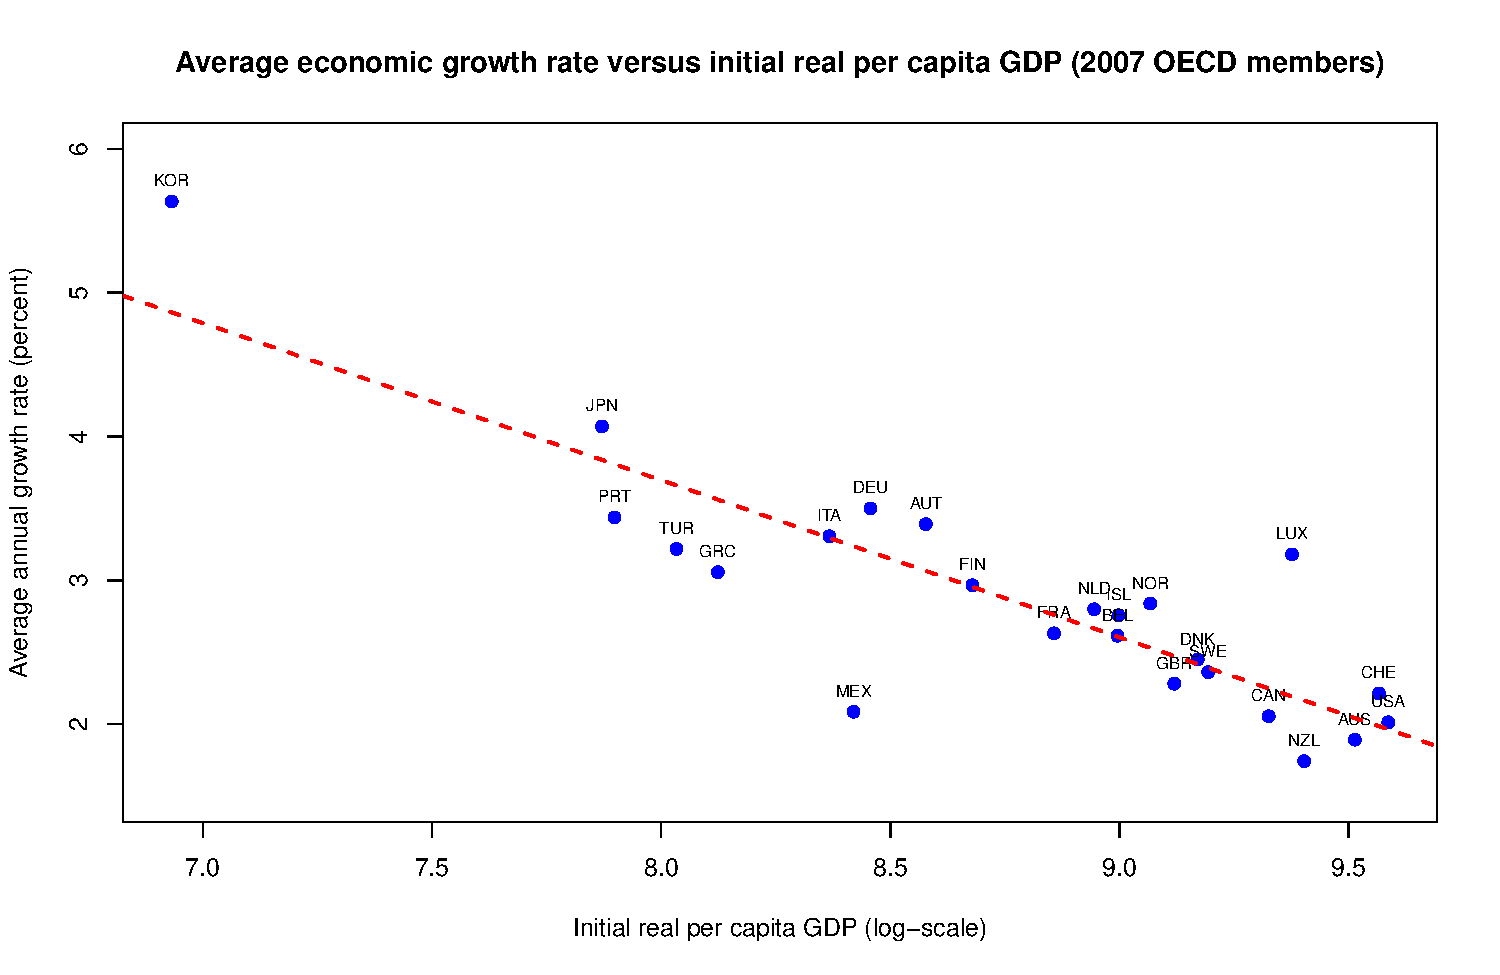
\includegraphics[width=0.7\linewidth]{week8/week8-growth9-1} 

\end{knitrout}
\end{center}

The previous graph shows that convergence may happen if we select the
countries wisely. The reason for selecting the countries based on
their OECD membership, is that OECD countries are similar in many
aspects. When we observe convergence among countries that share
similar characteristics, we call it conditional convergence because
the convergence is conditional on the countries having some
similarities. 

The economic growth theory provides a possible list of characteristics
that need to be similar for countries to converge to each other. In
this chapter we only explore a few: education, literacy and
health. The following scatter plots include countries with the
following characteristics: life expectancy greater than 60 years (top
left), the education level of more than 30\% of adults is at least
upper secondary (top right), the proportion of literacy is greater
than 80\% (bottom left) and all previous three characteristics are
satisfied (bottom right). The data on education, literacy and life
expectancy are from Characteristics.csv file. In order to see that
OECD members share those characteristics, which may explain why
convergence exists among them, they are represented on the graphs by
red squares. The main result is that convergence exists on average
among countries with favorable characteristics (good education, good
health etc.): the red dashed lines shows that the comovements are
negative on average. However, the large variations suggest that being
healthy and educated is not sufficient for poor countries to grow
fast.
\begin{center}
\begin{minipage}{.45\textwidth}
\begin{knitrout}\footnotesize
\definecolor{shadecolor}{rgb}{0.969, 0.969, 0.969}\color{fgcolor}
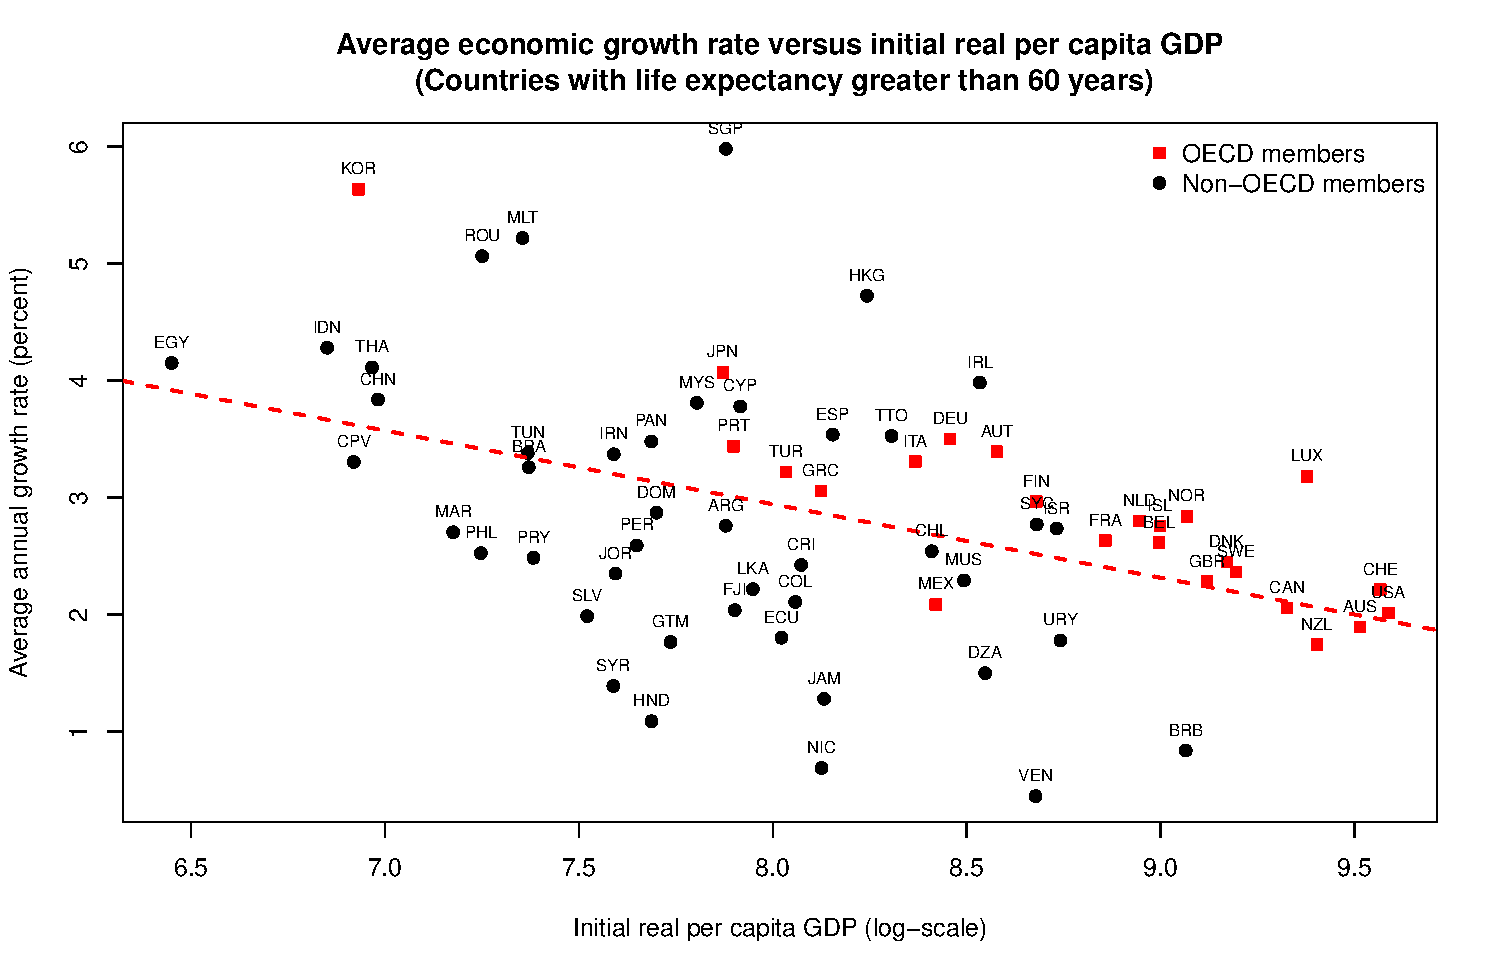
\includegraphics[width=\maxwidth]{week8/week8-growth10-1} 

\end{knitrout}
\end{minipage}
\begin{minipage}{.45\textwidth}
\begin{knitrout}\footnotesize
\definecolor{shadecolor}{rgb}{0.969, 0.969, 0.969}\color{fgcolor}
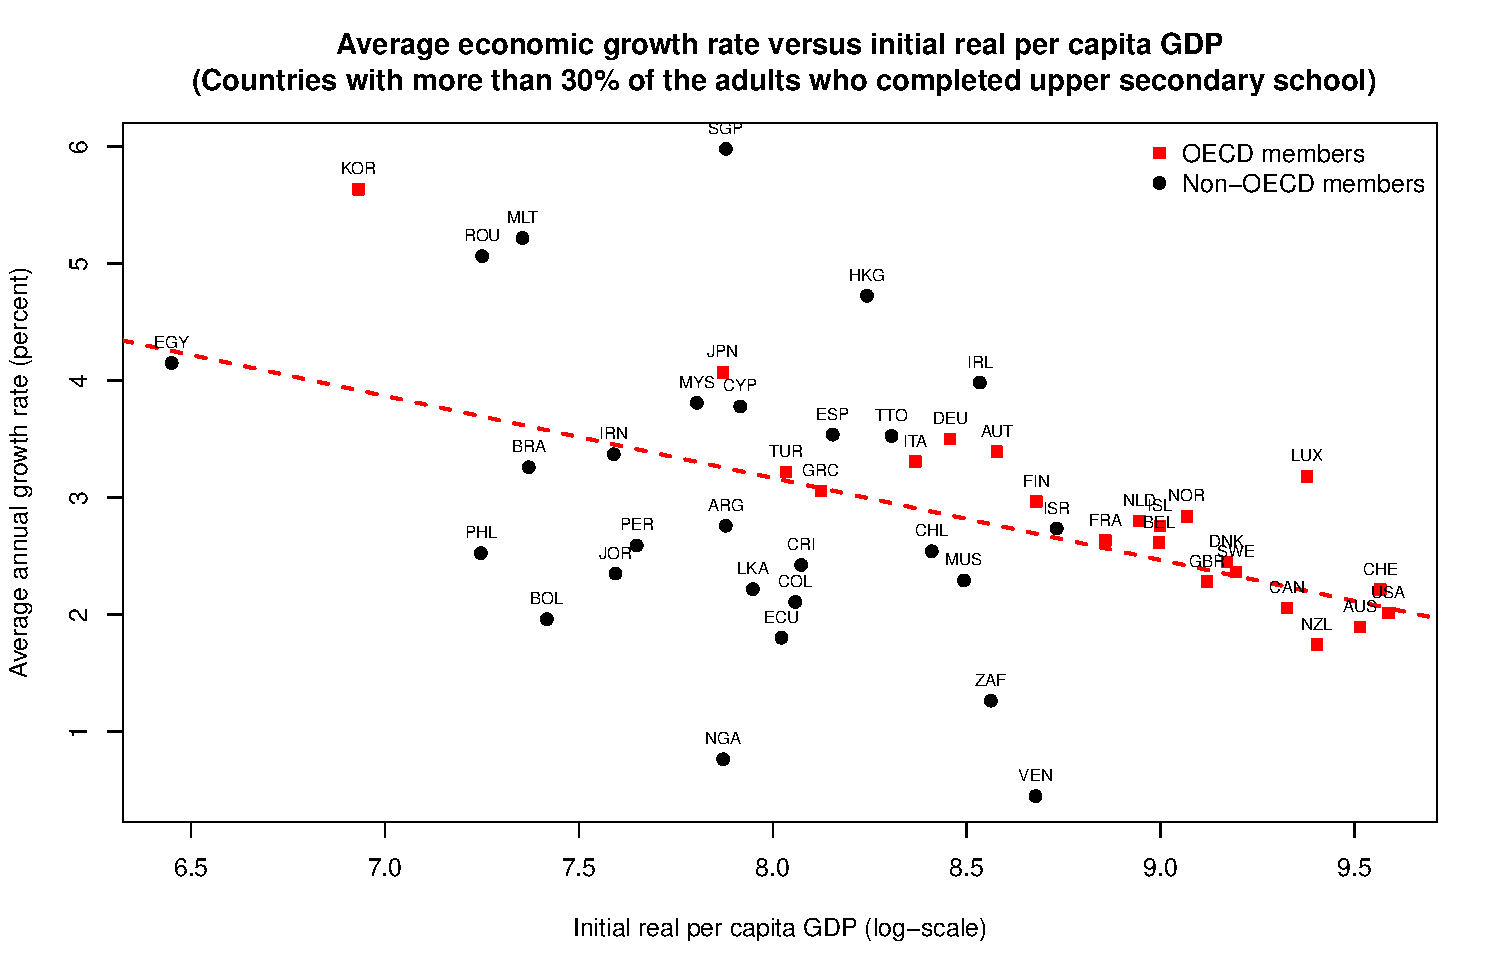
\includegraphics[width=\maxwidth]{week8/week8-growth11-1} 

\end{knitrout}
\end{minipage}
\end{center}

\begin{center}
\begin{minipage}{.45\textwidth}
\begin{knitrout}\footnotesize
\definecolor{shadecolor}{rgb}{0.969, 0.969, 0.969}\color{fgcolor}
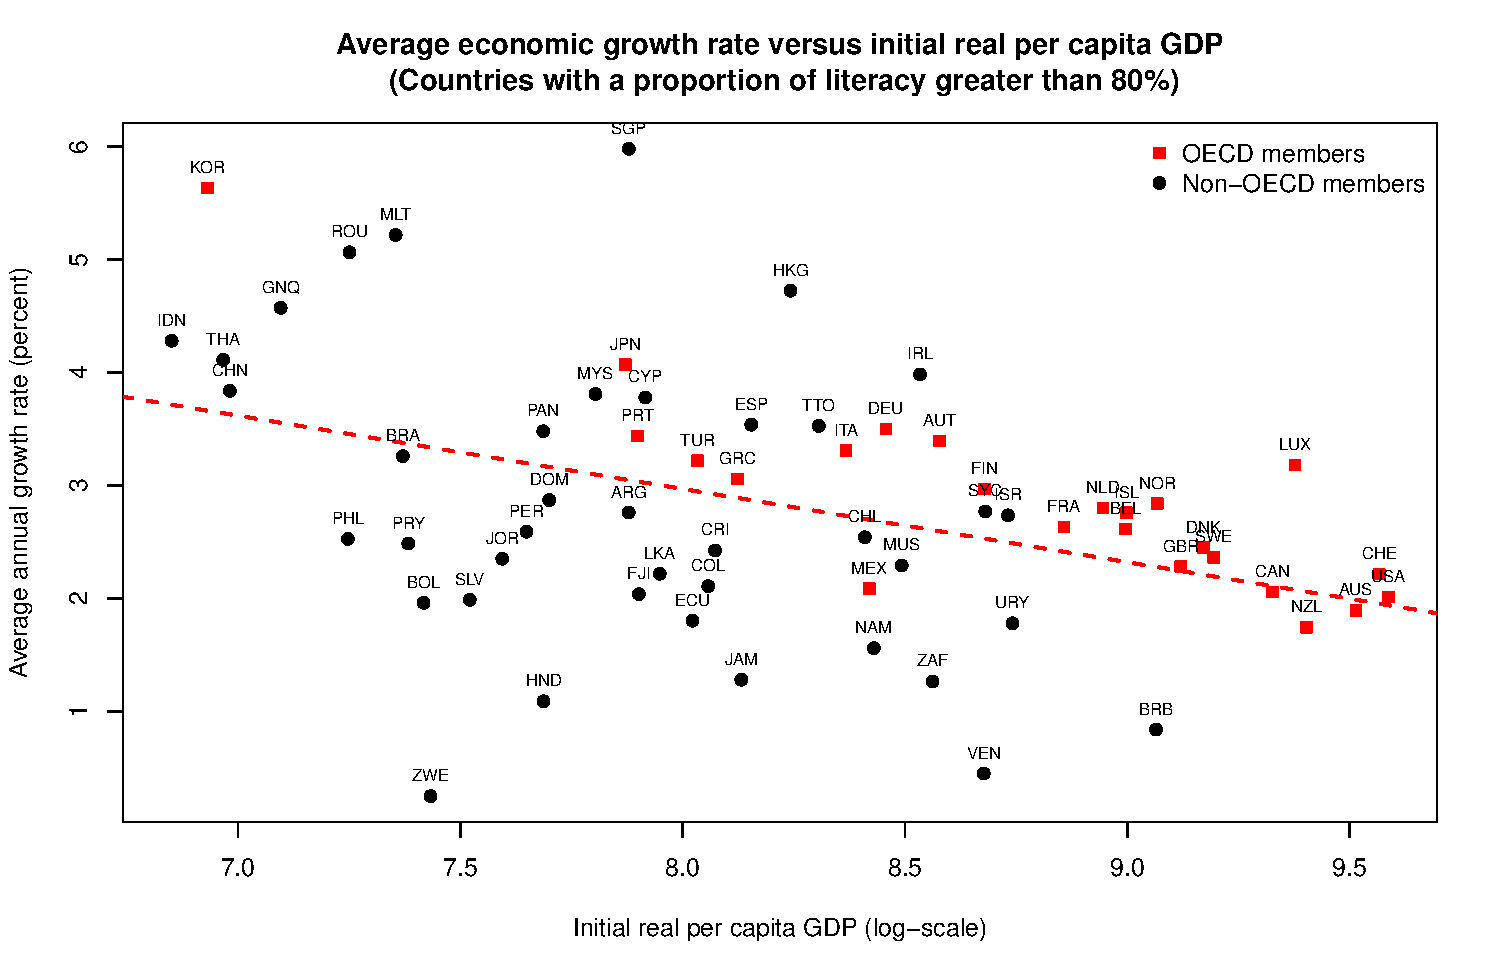
\includegraphics[width=\maxwidth]{week8/week8-growth12-1} 

\end{knitrout}
\end{minipage}
\begin{minipage}{.45\textwidth}
\begin{knitrout}\footnotesize
\definecolor{shadecolor}{rgb}{0.969, 0.969, 0.969}\color{fgcolor}
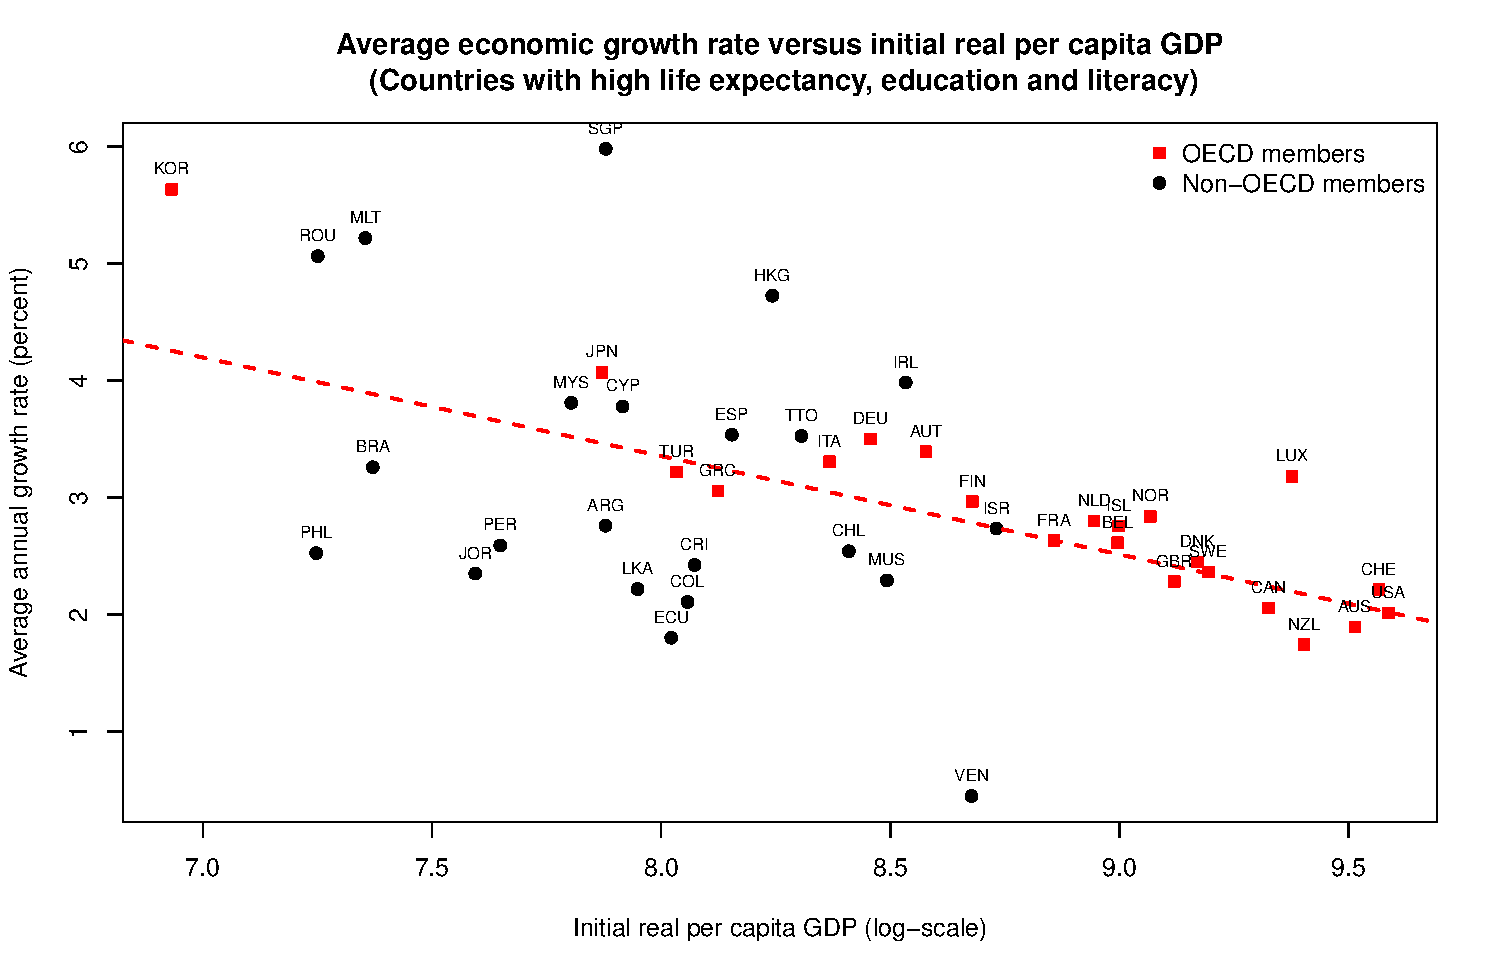
\includegraphics[width=\maxwidth]{week8/week8-growth13-1} 

\end{knitrout}
\end{minipage}
\end{center}
To conclude this section, we want to consider convergence conditioned
on the level of economic freedom. What is economic freedom and why it
may have an impact on growth and the standard of living? Watch the
following short videos to understand what it means:
\begin{itemize}
\item \href{https://youtu.be/3_HnZa2XSrc}{Fraser Institute: The Benefits of Economic Freedom} (1:51 min)
\item \href{https://youtu.be/SgXeOTBiPZI}{Women's Economic Rights—What's Changed and Why Does It Matter?} (1:09 min)  
\end{itemize}
The Fraser Institute constructs an economic freedom index
\citep*{freedom} which is based on 44 variables covering topics such
as legal system, security of property rights, freedom of trade,
regulation etc. The index goes from 0 (absence of freedom) to 10
(total freedom). If you are interested to know how it is constructed,
you can visit their
\href{https://www.fraserinstitute.org/economic-freedom/approach}{website}. This
is an index that puts different weights of different freedom
measures. You may or may not agree with their view of what freedom
means. In fact, you should always be skeptical about such measures and
verify by yourself how they are constructed. An interesting results,
however, is the strong positive comovement between the economic
freedom index and the inequality adjusted human development index
(IHDI) as we can see on the following graph. In particular, most
countries with an economic freedom index greater than 7.2 have a
relatively high IHDI. However, some countries have an economic freedom
index around 7 and a very low IHDI.

\begin{minipage}{.75\textwidth}  
\begin{knitrout}\footnotesize
\definecolor{shadecolor}{rgb}{0.969, 0.969, 0.969}\color{fgcolor}
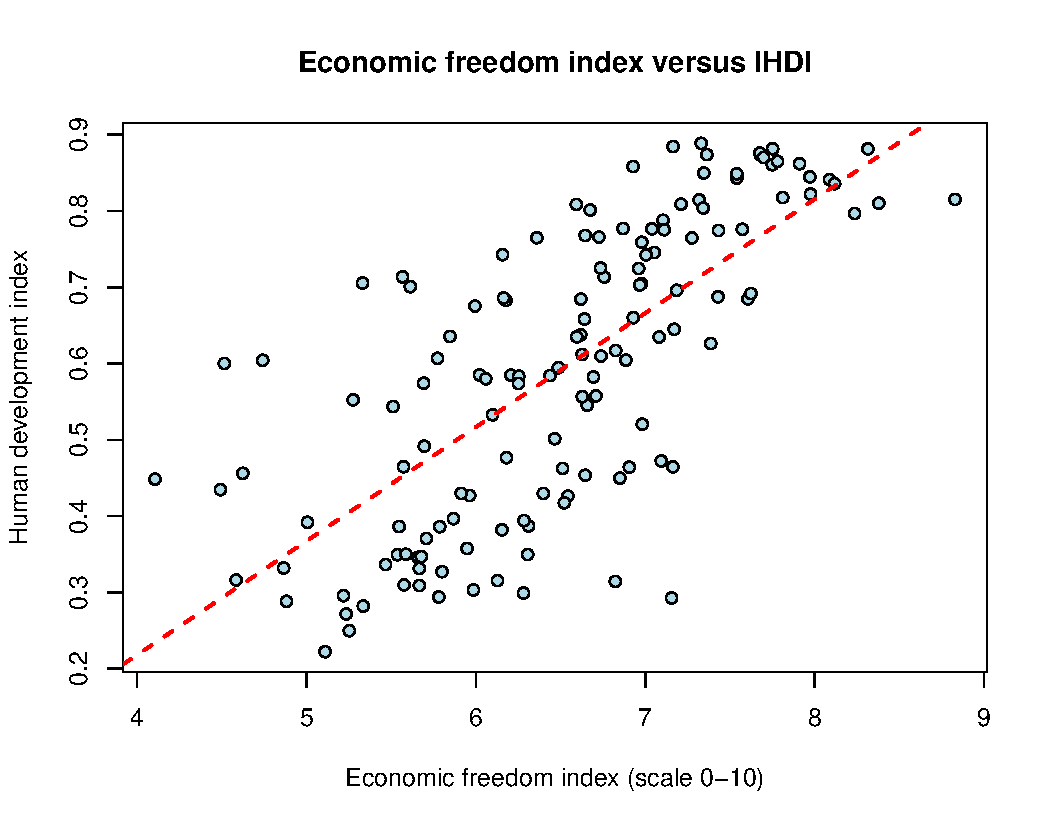
\includegraphics[width=\maxwidth]{week8/week8-ihdi_freedom-1} 

\end{knitrout}
\end{minipage}

The series of the indexes for several countries from 1970 to 2017 are
included in the EconFreedom.csv file. According to the index, for
example, the country with the highest economic freedom in 2017 was
Hong Kong with 8.91, and Venezuela was the country with the lowest
score with 2.58. The following graphs are scatter plots of economic
growth with respect to initial real per capita GDP for countries with
an economic freedom greater than the median 6.5 (left graph) and less
than 6.5 (right graph) on average over the period 1970-2017. We
observe more convergence among countries with higher economic
freedom (stronger negative comovement). But again, we see lots of
variations: countries with a higher economic freedom index do not
necessarily converge to rich countries.
\begin{center}
\begin{minipage}{.45\textwidth}
\begin{knitrout}\footnotesize
\definecolor{shadecolor}{rgb}{0.969, 0.969, 0.969}\color{fgcolor}
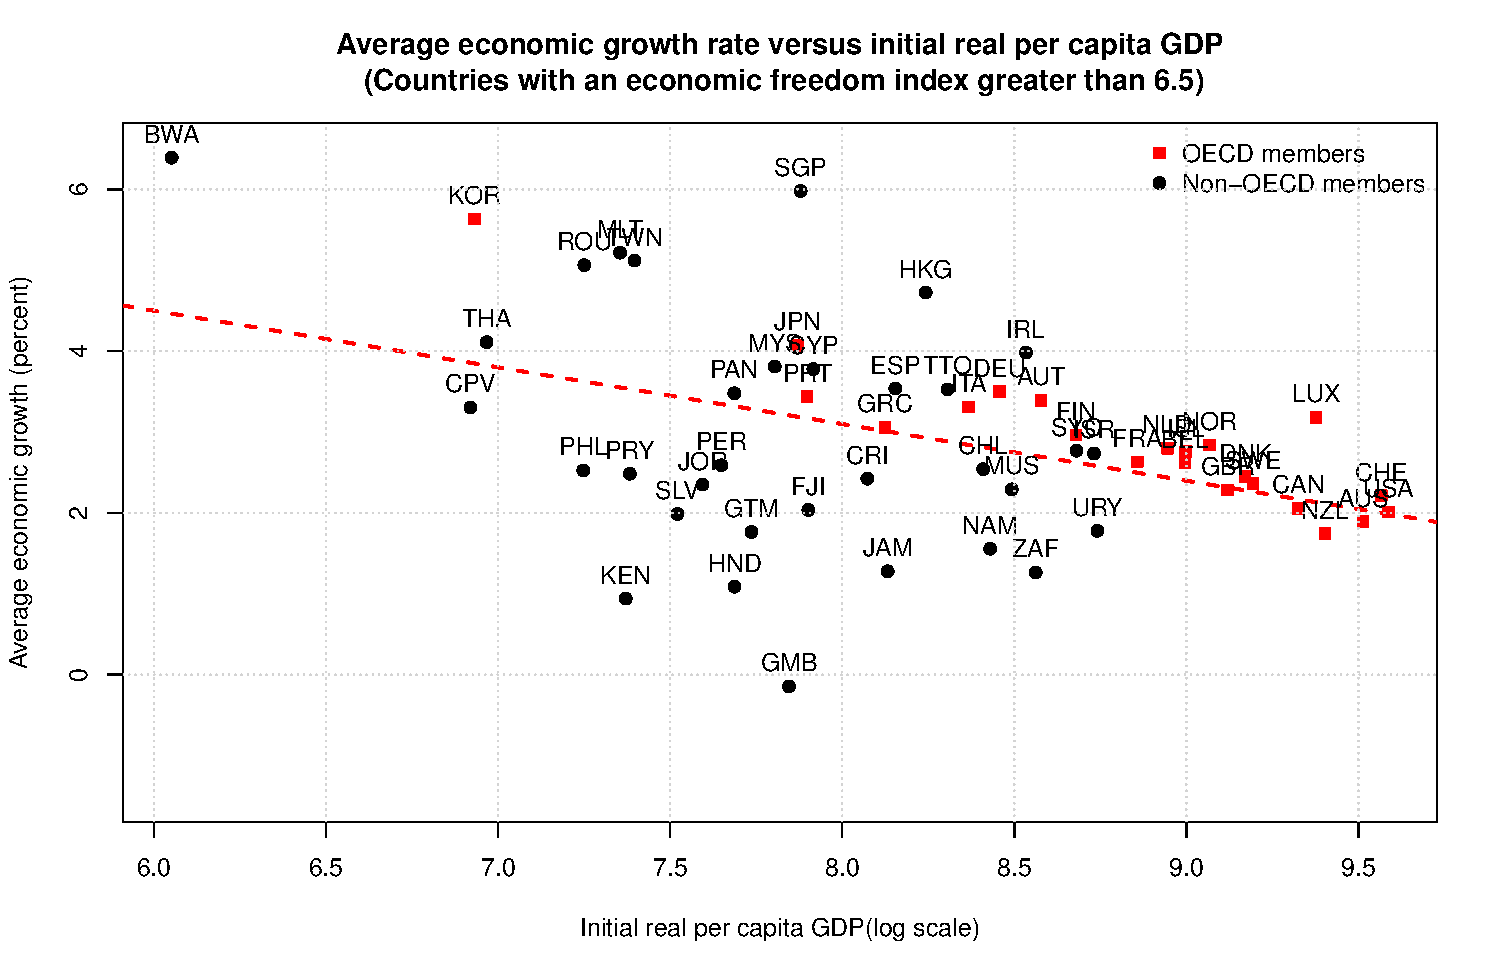
\includegraphics[width=\maxwidth]{week8/week8-growth14-1} 

\end{knitrout}
\end{minipage}
\begin{minipage}{.45\textwidth}
\begin{knitrout}\footnotesize
\definecolor{shadecolor}{rgb}{0.969, 0.969, 0.969}\color{fgcolor}
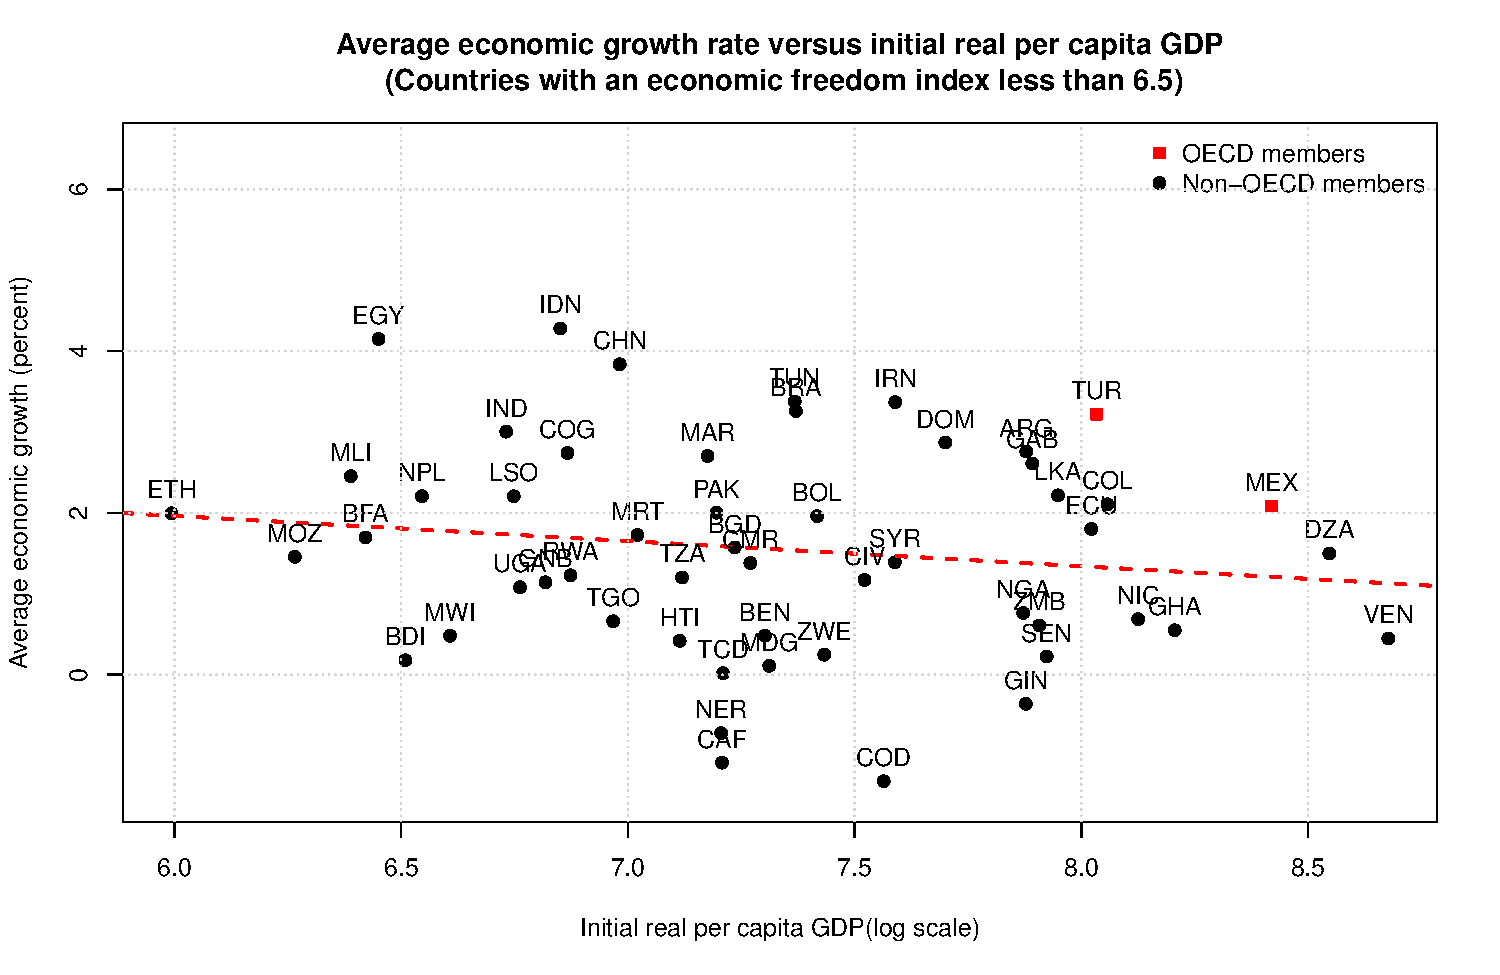
\includegraphics[width=\maxwidth]{week8/week8-growth15-1} 

\end{knitrout}
\end{minipage}
\end{center}
Notice that we cannot conclude that any of the variables analyzed in
this section help poor countries become richer. We did observe a
relationship between education, health, economic freedom and the
ability of poor countries to grow, but observing comovements does not
imply that an actual relationship exists. Also, the variations that we
observe in all graphs suggests that we need to dig deeper to
understand why some poor countries grow and others remain
poor. Answering those questions is the topic of economic growth and
development courses.


\subsection{Determinants of Economic Growth}

The title of the section is a little too ambitious given the tools
that we have at hand. Only theory and/or advanced statistical
techniques can identify what determine growth. You may find that I am
repeating myself, but I want to make sure you remember that comovement
and relationship are two completely different things. 

In this section we want to analyze the comovement between economic
growth and some characteristics. In the following scatter plots
average economic growth is on the y-axis and the country
characteristics obtained from the Characteristics.csv file are on the
x-axis. First, we want to see if a comovement exists between economic
growth and some economic variables. The first set of variables are the
government share (G divided by GDP) on the top left graph, the
investment share (I divided by GDP) on the top right graph and the
level of openness (X+M divided by GDP) on the bottom graph. On each
graph, the OECD countries are represented by the dark blue squares and
all other countries by the light blue bullets. We observe a positive
comovement in all graph (shown by the red dashed line), but the it is
stronger for the investment share and level of openness than for the
share of government spending. Economic theory would suggest that
investment and trade are good for growth. Therefore, the graphs are in
line with the theory (without proving it of course).

\begin{center}
\begin{minipage}{.45\textwidth}
\begin{knitrout}\footnotesize
\definecolor{shadecolor}{rgb}{0.969, 0.969, 0.969}\color{fgcolor}
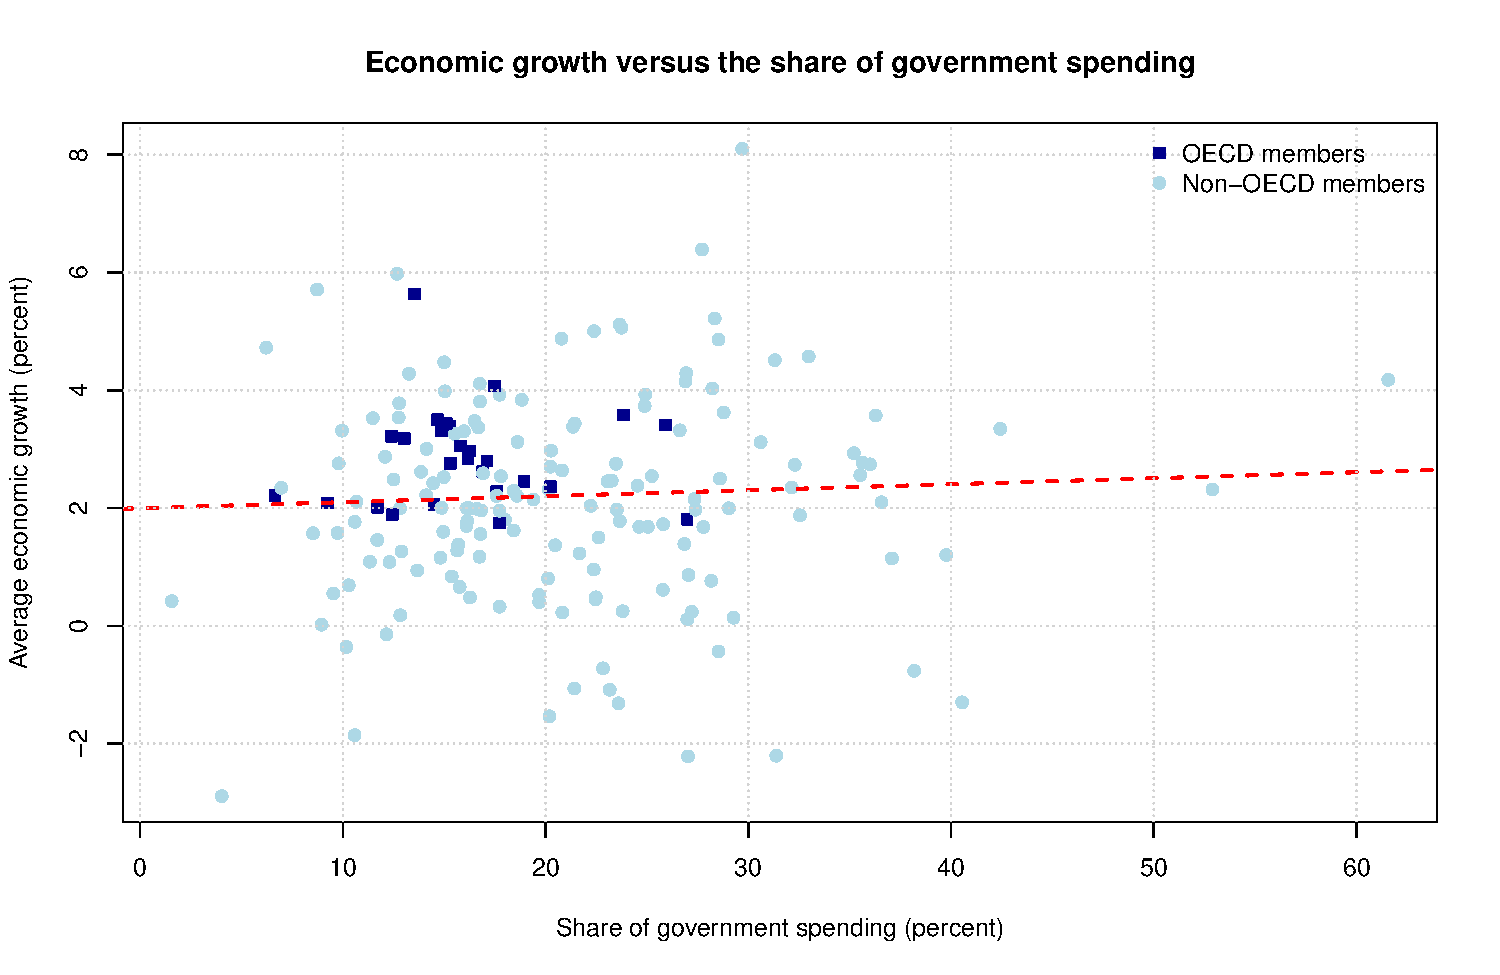
\includegraphics[width=\maxwidth]{week8/week8-det1-1} 

\end{knitrout}
\end{minipage}
\begin{minipage}{.45\textwidth}
\begin{knitrout}\footnotesize
\definecolor{shadecolor}{rgb}{0.969, 0.969, 0.969}\color{fgcolor}
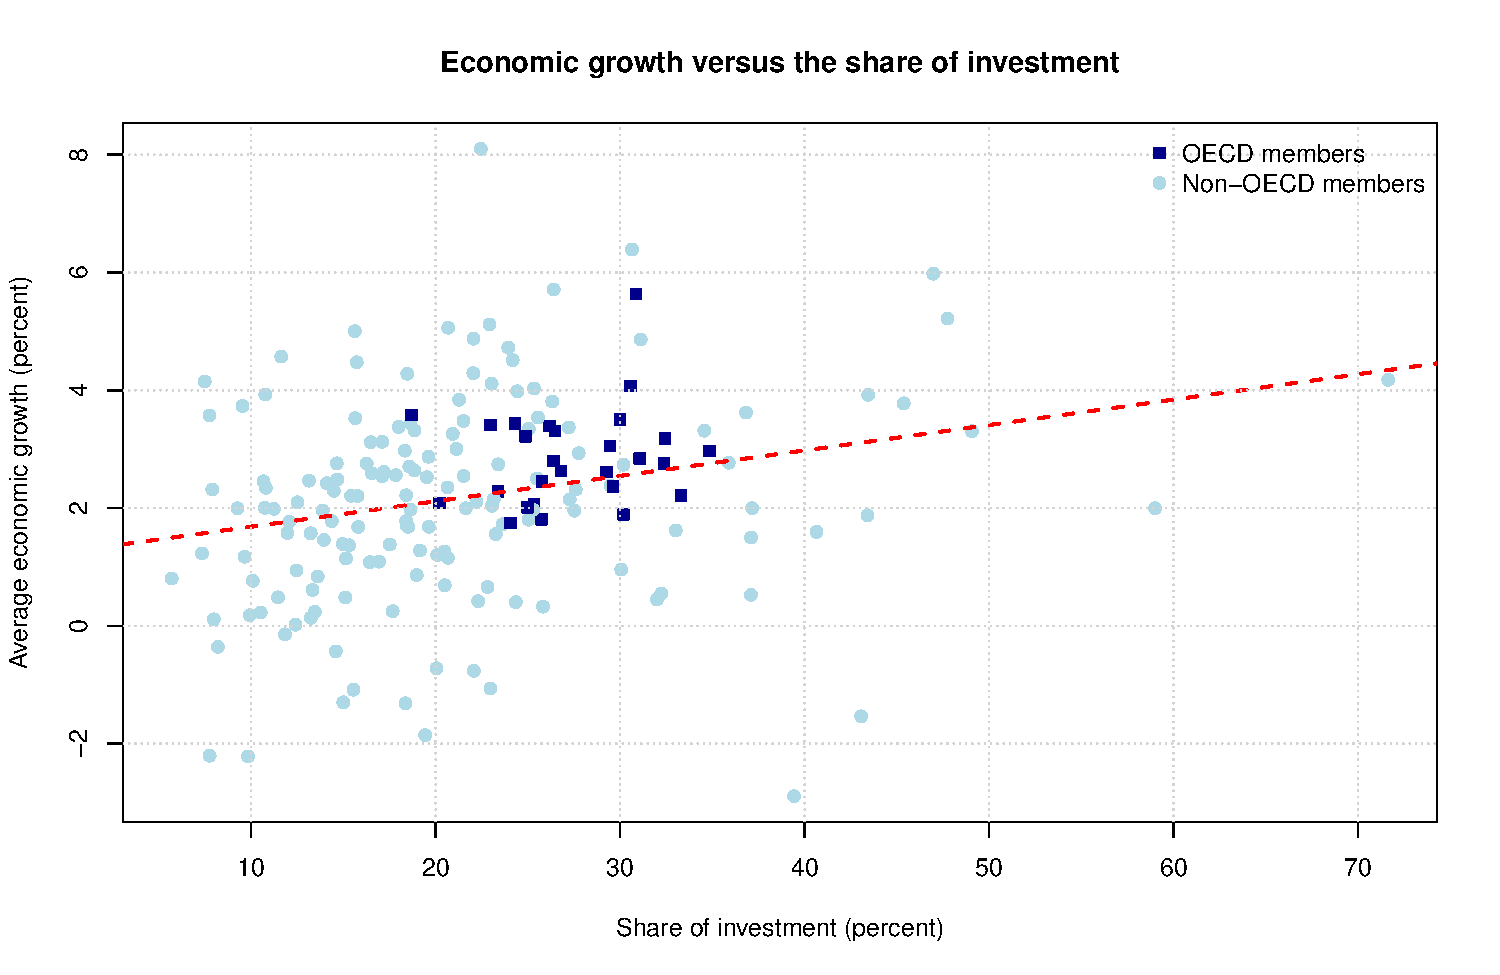
\includegraphics[width=\maxwidth]{week8/week8-det2-1} 

\end{knitrout}
\end{minipage}
\end{center}

\begin{center}
\begin{minipage}{.45\textwidth}
\begin{knitrout}\footnotesize
\definecolor{shadecolor}{rgb}{0.969, 0.969, 0.969}\color{fgcolor}
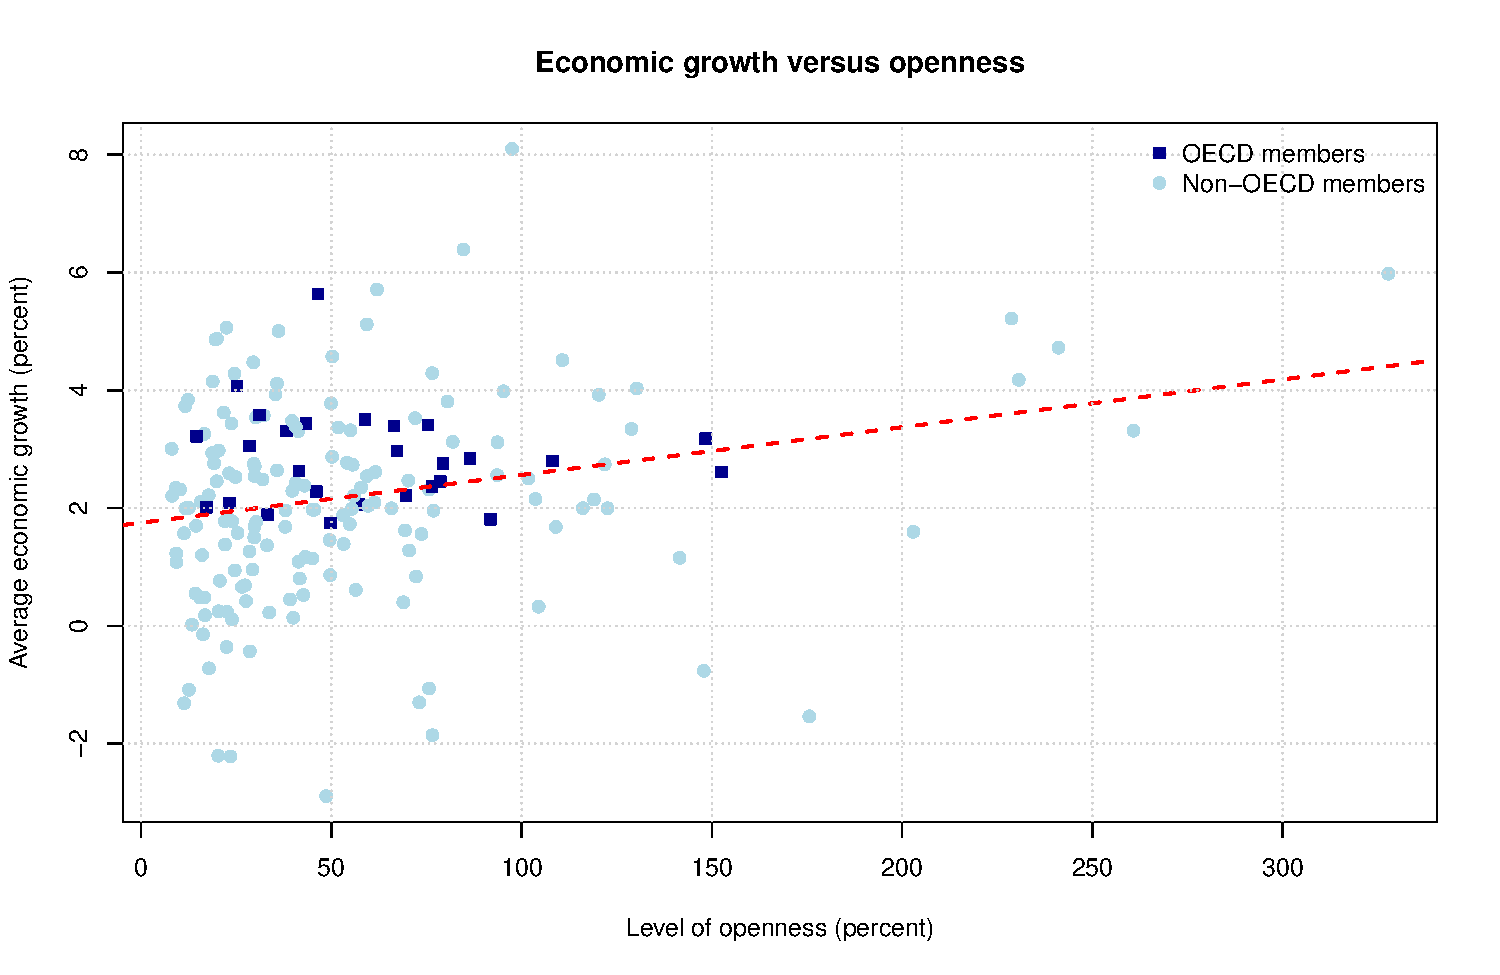
\includegraphics[width=\maxwidth]{week8/week8-det3-1} 

\end{knitrout}
\end{minipage}
\end{center}

For the next set of graphs, we want to see if we observe a comovement
between economic growth and education (the top right graph), literacy
(the bottom graph) and health (the top right graph). We also observe a
positive comovement between those variables and the economic
growth. It is less strong for the education measure, but we used a
narrowed measure of education. 
\begin{center}
\begin{minipage}{.45\textwidth}
\begin{knitrout}\footnotesize
\definecolor{shadecolor}{rgb}{0.969, 0.969, 0.969}\color{fgcolor}
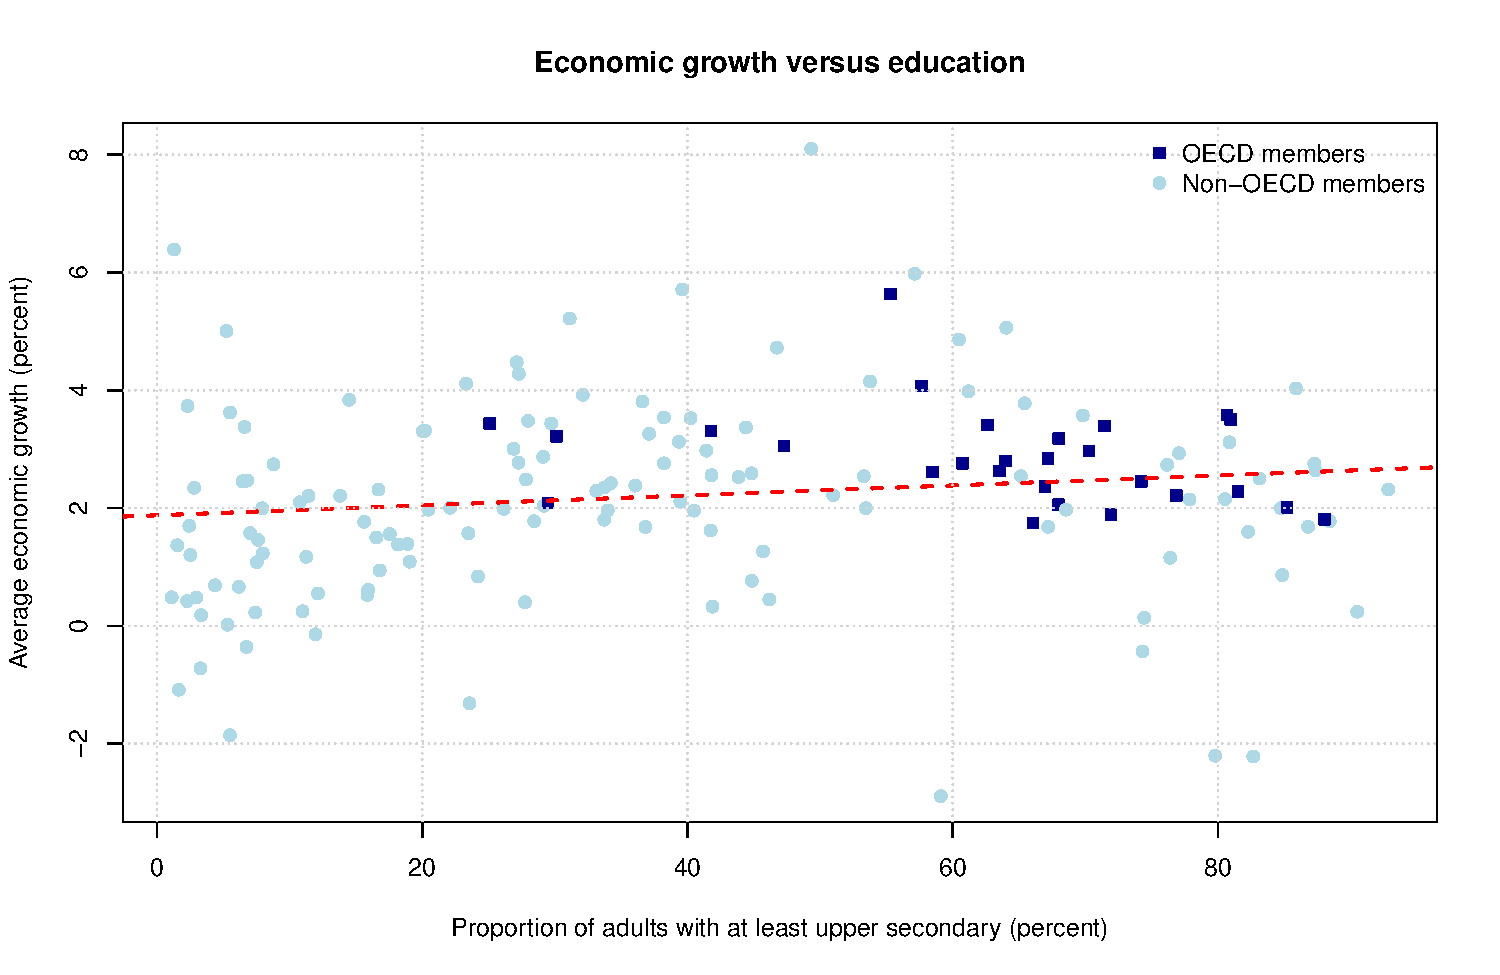
\includegraphics[width=\maxwidth]{week8/week8-det4-1} 

\end{knitrout}
\end{minipage}
\begin{minipage}{.45\textwidth}
\begin{knitrout}\footnotesize
\definecolor{shadecolor}{rgb}{0.969, 0.969, 0.969}\color{fgcolor}
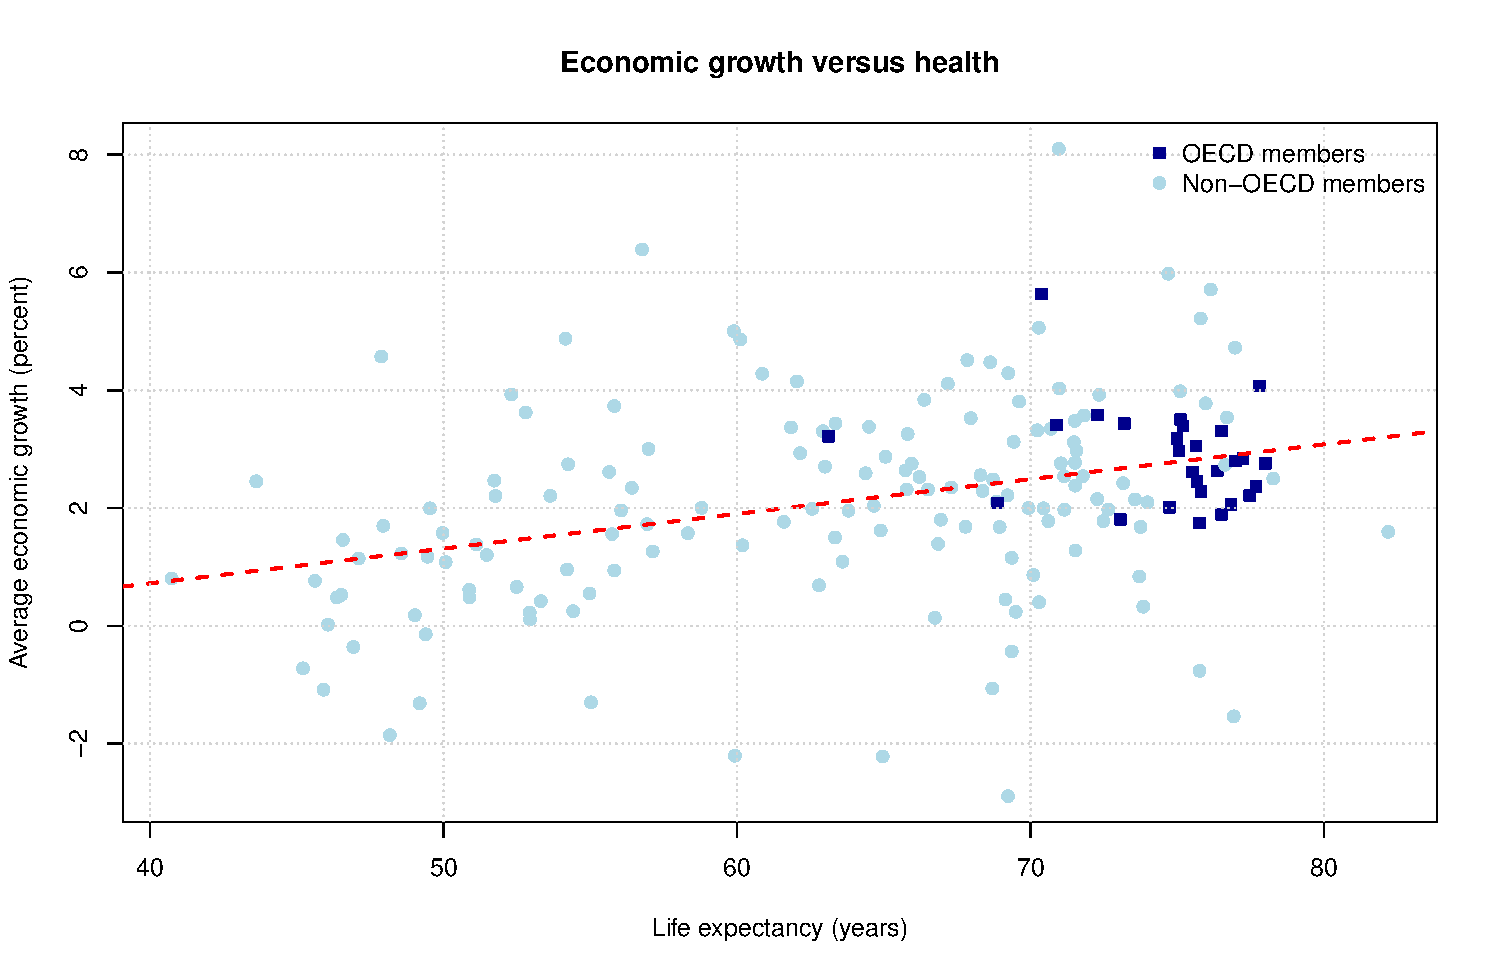
\includegraphics[width=\maxwidth]{week8/week8-det5-1} 

\end{knitrout}
\end{minipage}
\end{center}

\begin{center}
\begin{minipage}{.45\textwidth}
\begin{knitrout}\footnotesize
\definecolor{shadecolor}{rgb}{0.969, 0.969, 0.969}\color{fgcolor}
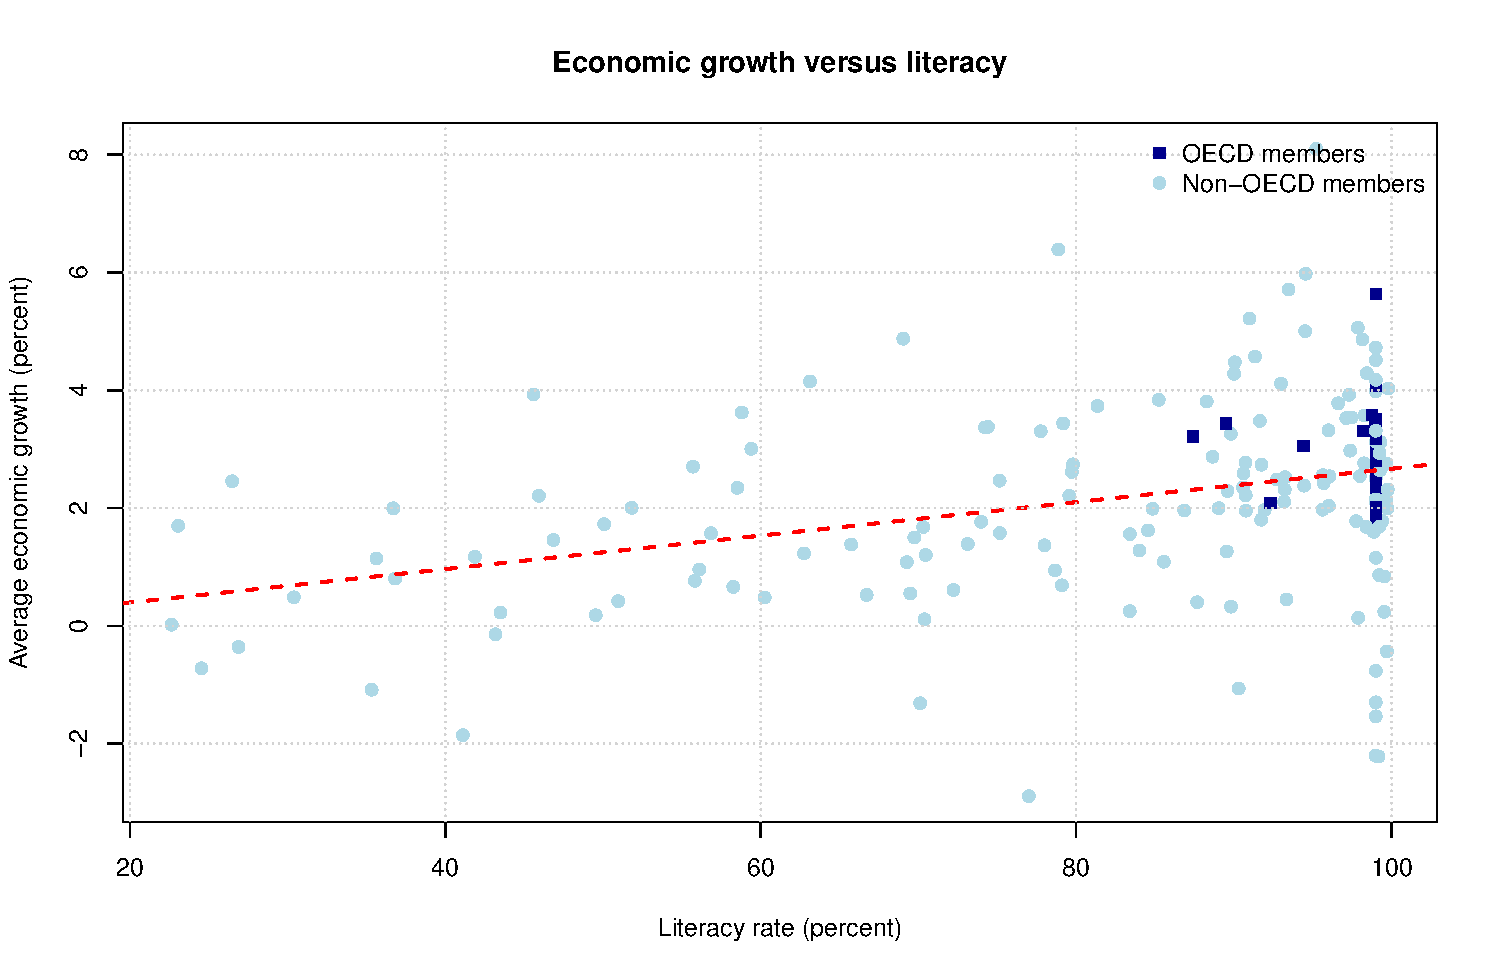
\includegraphics[width=\maxwidth]{week8/week8-det6-1} 

\end{knitrout}
\end{minipage}
\end{center}

We conclude this section by analyzing the comovement between average
economic growth and the economic freedom index. The purpose of
presenting this variable is to emphasize the fact the economic growth
and development is not only affected by economic
variables. Characteristics such as the political system, the social
norms and the legal system also play a role in a country
development. The scatter plot shows that there is a positive
comovement between growth and economic freedom. However, it is
possible for countries with a relatively high level of economic
freedom to have a low economic growth. See for example Georgia (GEO)
and Gambia (GMB). The United Arab Emirates (ARE) is an outlier (a
country very different from the rest) because its real per capita GDP
went from 252 thousand in 1970 to 66 thousand in 2017. That can be
explained by the fact that the proportion of GDP that was coming from
oil production went from more than 40\% in 1970 to about 10\% in 2017
(source, World Bank) while the population went from half a million to
9.4 million. The Gini coefficient is not available for that country,
but we should expect a high level of income inequality in 1970.

\begin{center}
\begin{minipage}{.75\textwidth}
\begin{knitrout}\footnotesize
\definecolor{shadecolor}{rgb}{0.969, 0.969, 0.969}\color{fgcolor}
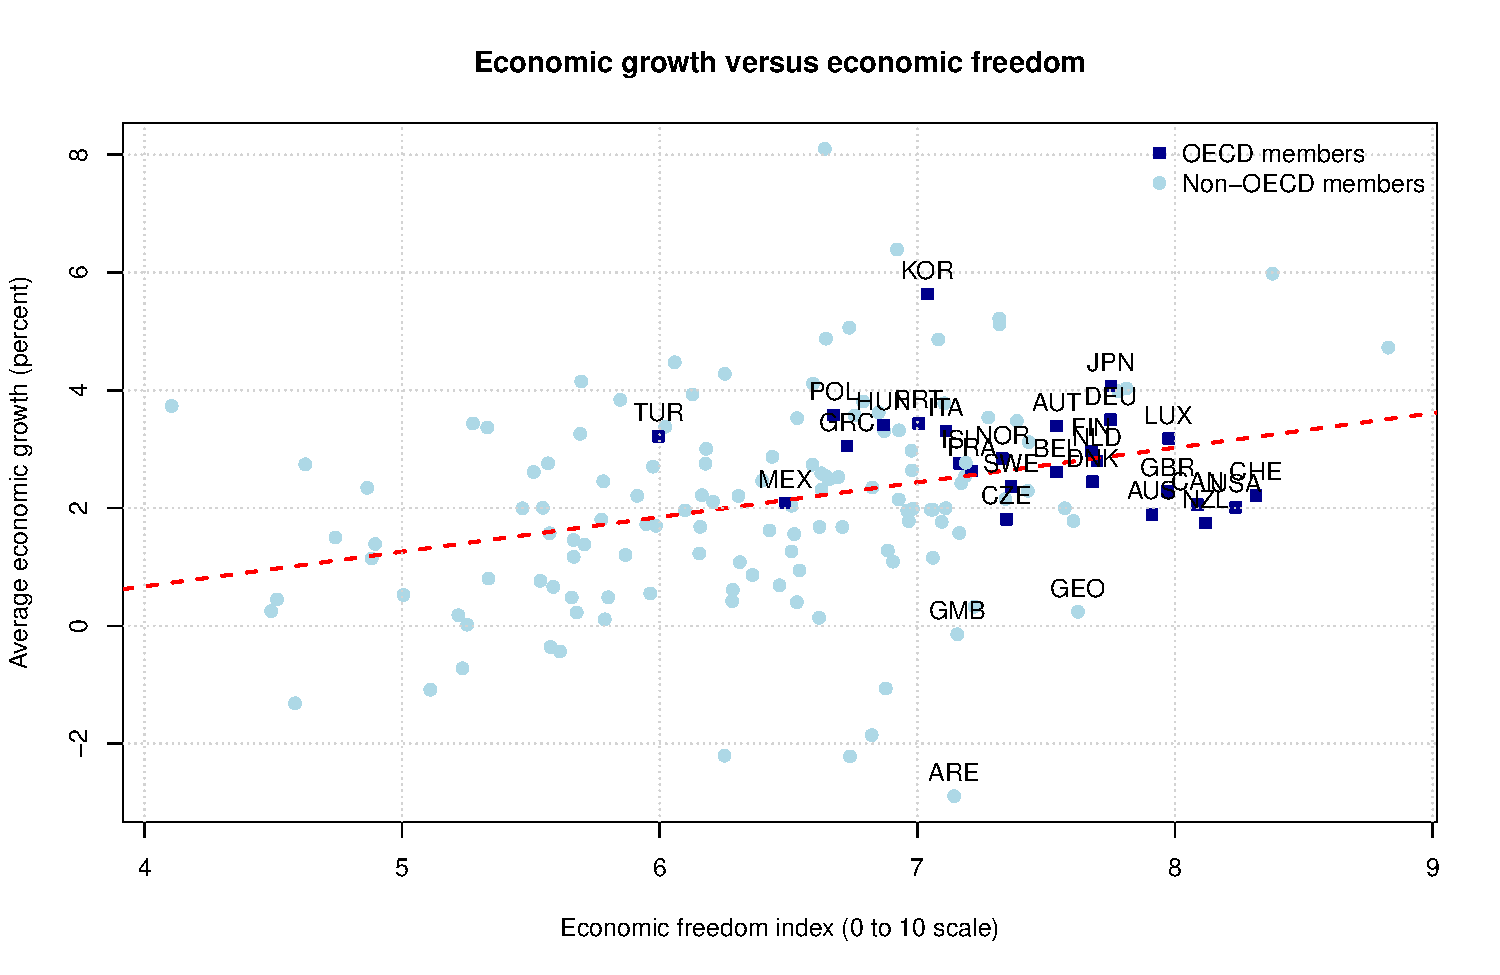
\includegraphics[width=\maxwidth]{week8/week8-det7-1} 

\end{knitrout}
\end{minipage}
\end{center}

\subsection{Concluding Remark}
In this section, we review the main findings of the chapter We went
through many facts regarding economic growth and it is important to
summarize the most important ones. 
\begin{itemize}
\item We use real per capita GDP as an indicator of welfare not
  because welfare only depends on it, but because countries with high
  real per capita GDP tend to have high values for variables that
  affect the quality of life. However, we have to keep in mind that
  the comovement is not perfect. Many countries have high real per
  capita GDP and low education and life expectancy.
\item The real per capita GDP has increased in most countries between
  1950 and 2017, but the inequality in the growth rates resulted in an
  increase of income inequality over the period. If we weight the
  country by their population to obtained the income distribution at
  the individual level, the increase of income inequality is
  reduced. This is mainly due to the fact that large countries such as
  China and India have experienced relatively high economic growth.
\item We do not observe unconditional convergence: globally, the
  standard of living of poor countries is not converging to the
  standard of living of rich countries.
\item We do observer conditional convergence: if we restrict our
  sample to countries with favorable characteristics (high education,
  life expectancy and economic freedom), we observe poor countries
  converging to rich countries on average. However, there is lots of
  variations which means that some poor countries with favorable
  characteristics do not grow enough to catch-up with the richer
  countries.
\item Economic growth seems to positively correlate (positive
  comovement) with investment, openness, health, education and
  economic freedom. However, the observed variations suggest that it
  is not sufficient to have high investment, openness, health,
  education and economic freedom to grow. 
\item All the facts that we analyzed in this chapter have policy
  implications. If we are willing to accept that growth is a solution
  to welfare improvement, then policies that promote economic growth
  are likely to be beneficial for a country. How do we promote growth?
  According to our results, if a poor country is able increase its
  education, investment, international trade, economic freedom and
  health, growth should increase on average. Also, by matching the
  characteristics of richer countries its standard of living should
  converge to the standard of living of the rich countries
  (conditional convergence). The effectiveness of these policies
  relies on the validity of our observed results. Unfortunately, what
  we discovered in this chapter is not sufficient to assess the
  effectiveness of policies. In order to propose or evaluate policies,
  we need to know more about the theory of economic growth and
  development, and we need stronger statistical foundation.

  \end{itemize}



\section{Exercises on Economic Growth}

\subsubsection*{Question 1}
Using the file WB\_LIFE.csv, compare the distribution of life
expectancy across countries in 1960 and 2018 using histograms. Add the
frequency on top of each bar. What is the proportion of countries with
life expectancy less than 50 years in 1960 and 2018?

\subsubsection*{Question 2}
\begin{enumerate}[a)]
\item The following graph is the histogram of real per capita GDP in 1990
using the density as measurement unit. Given that the number of
countries is equal to 180 and the interval length of each bar is 0.5,
what is the proportion and the number of countries that have a log per
capita real GDP between 8.5 and 9.0?

\begin{center}
\begin{minipage}{.65\textwidth}
\begin{knitrout}\footnotesize
\definecolor{shadecolor}{rgb}{0.969, 0.969, 0.969}\color{fgcolor}
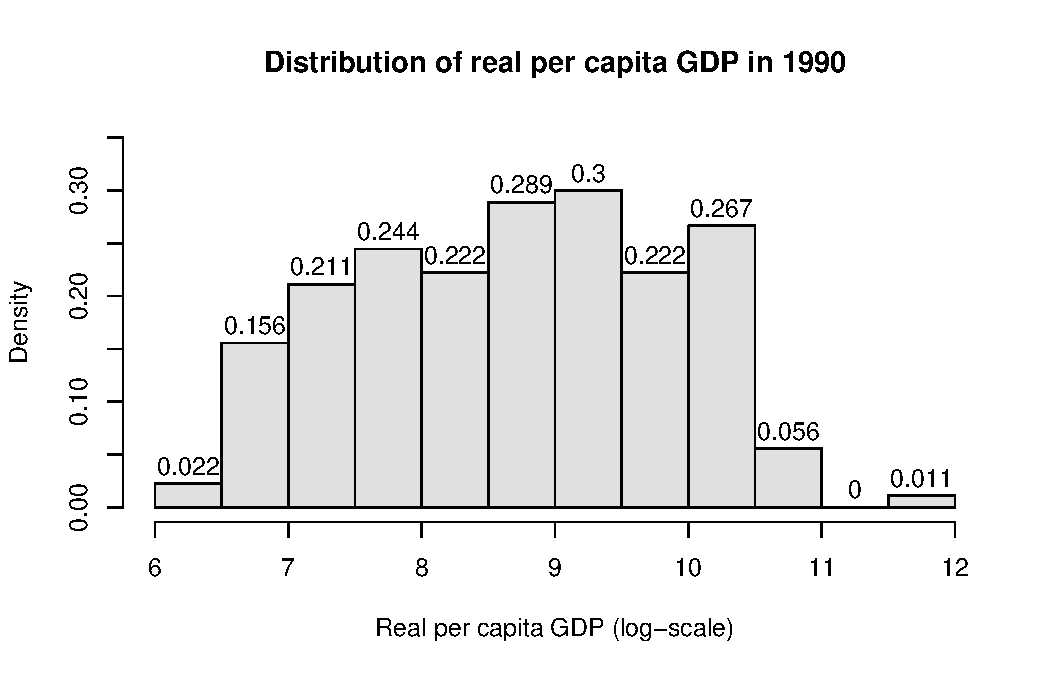
\includegraphics[width=\maxwidth]{week8/week8-ex1-1} 

\end{knitrout}
\end{minipage}
\end{center}
\item The following is the same distribution with the y-axis expressed
  in the number of countries and the x-axis in thousands of
  international dollars of 2011. The number of bars has also been
  increased. Given that the number of countries is equal to 180 and
  the interval length for each bar is 5, what is the density value of
  the first bar? What is the main difference between the histogram in
  a) and b)?
\begin{center}
\begin{minipage}{.65\textwidth}
\begin{knitrout}\footnotesize
\definecolor{shadecolor}{rgb}{0.969, 0.969, 0.969}\color{fgcolor}
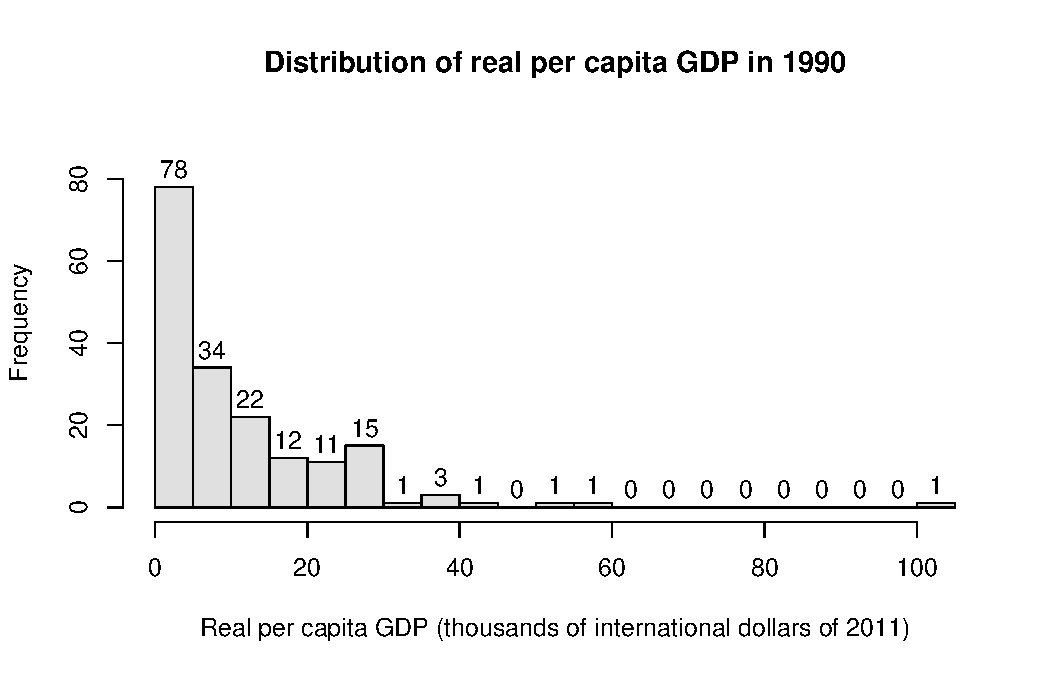
\includegraphics[width=\maxwidth]{week8/week8-ex2-1} 

\end{knitrout}
\end{minipage}
\end{center}  

\item The following table shows the average real per capita GDP in
  logs and thousands of dollars per quintile.
\begin{center}
\resizebox{0.8\linewidth}{!}{  
% latex table generated in R 3.6.3 by xtable 1.8-4 package
% Fri May 15 16:13:01 2020
\begin{tabular}{l|cc}
  \multicolumn{3}{c}{Average real per capita GDP per quintile}\\ \hline
 & Real per capita GDP (thousands of dollars) & Real per capita GDP (logs) \\ 
  \hline
First quintile & 1.14 & 7.00 \\ 
  Second quintile & 2.92 & 7.95 \\ 
  Third quintile & 6.39 & 8.74 \\ 
  Fourth quintile & 12.86 & 9.44 \\ 
  Fifth quintile & 30.20 & 10.24 \\ 
   \hline
\end{tabular}

}
\end{center}  
\end{enumerate}
Using the information in the table, explain why the distribution of
the variable expressed in thousands of dollars is skewed while it is
not (or almost not) when it is expressed in logs.

\subsubsection*{Question 3}
The following is the list of countries that were members of the
European Union (EU) in 2013.
\begin{center}
\resizebox{0.8\linewidth}{!}{    
% latex table generated in R 3.6.3 by xtable 1.8-4 package
% Fri May 15 16:13:01 2020
\begin{tabular}{llll}
  \hline
  \hline
Austria (AUT) & Estonia (EST) & Italy (ITA) & Portugal (PRT) \\ 
  Belgium (BEL) & Finland (FIN) & Latvia (LVA) & Romania (ROU) \\ 
  Bulgaria (BGR) & France (FRA) & Lithuania (LTU) & Slovakia (SVK) \\ 
  Croatia (HRV) & Germany (DEU) & Luxembourg (LUX) & Slovenia (SVN) \\ 
  Cyprus (CYP) & Greece (GRC) & Malta (MLT) & Spain (ESP) \\ 
  Czech Republic (CZE) & Hungary (HUN) & Netherlands (NLD) & Sweden (SWE) \\ 
  Denmark (DNK) & Ireland, Republic of (EIRE) (IRL) & Poland (POL) & United Kingdom (GBR) \\ 
   \hline
\end{tabular}

}
\end{center}

\begin{enumerate}[a)]
  \item For this question, consider only the EU countries for which
    the 1950 real per capita GDP was available (the InitYear is 1950
    in the Characteristics.csv file). Select the two countries with
    the lowest initial real per capita GDP and two with the
    highest. Then, plot the real per capita GDP of the four countries
    on the same chart for the period 1950-2017. Do you see poor
    countries converging to the richer countries?
  \item Answer question a), but express the real per capita GDP's in
    logs.
  \item Using all EU countries, create a scatter plot with the average
    growth rate on the y-axis and the initial real per capita GDP on
    the x-axis. Do you observe a global convergence among EU
    countries?
  \item Given the comovement between growth and other economic
    variables observed in the chapter, can you give a possible
    explanation of why Ireland (IRL) has grown faster than Italy (ITA)
    despite its initially higher real per capita GDP? How certain are
    you of your answer? Use the information included in the
    Characteristics.csv file.
\end{enumerate}

\subsubsection*{Question 4}
The following are the countries from West Africa. They are all
included in our data files.
\begin{center}
\resizebox{0.8\linewidth}{!}{    
% latex table generated in R 3.6.3 by xtable 1.8-4 package
% Fri May 15 16:13:01 2020
\begin{tabular}{llll}
  \hline
  \hline
Benin (BEN) & Ghana (GHA) & Liberia (LBR) & Nigeria (NGA) \\ 
  Burkina Faso (BFA) & Guinea (GIN) & Mali (MLI) & Senegal (SEN) \\ 
  Côte d'Ivoire (CIV) & Gambia (GMB) & Mauritania (MRT) & Sierra Leone (SLE) \\ 
  Cabo Verde (CPV) & Guinea-Bissau (GNB) & Niger (NER) & Togo (TGO) \\ 
   \hline
\end{tabular}

}
\end{center}
\begin{enumerate}[a)]
  \item Select the two countries with the lowest initial real per
    capita GDP, two with the highest and Cabo Verde (CPV). Then, plot
    the real per capita GDP of the four countries on the same chart
    for the period available. Do you see poor countries converging to
    the richer countries?
  \item Answer question a), but express the real per capita GDP's in
    logs.
  \item Create a scatter plot with the average growth rate on the
    y-axis and the initial real per capita GDP on the x-axis. Do you
    observe a global convergence among EU countries?
  \item Given the comovement between growth and other economic
    variables observed in the chapter can you give a possible
    explanation of why the growth rate of Capo Verde is so high while
    it is negative for Niger (NER) and Guinea (GIN)? How certain are
    you of your answer? Use the information included in the
    Characteristics.csv and EconFreedom.csv file.
\end{enumerate}

\subsubsection*{Question 5}
For the following questions, you will need the following formula: let
$X_0$ be the initial value, $X_t$ be the value after $t$ periods and
$g$ be the growth rate by period, then
\[
X_t = X_0(1+g)^t\,.
\]
You may also need the log properties: $\log(a^b)=b\log(a)$ and
$\log(ab)=\log(a)+\log(b)$. The properties imply:
\[
\log(X_t) = \log(X_0) + t\log(1+g)\,.
\]
\begin{enumerate}[a)]
\item Suppose the initial real per capita GDP for countries A and B is 
  5 thousand dollars. If the annual growth rates of countries A and B
  are respectively 1\% and 2\%, what is the the ratio $X_B/X_A$ after
  60 years? Interpret the result.
\item Suppose the annual growth rates of countries A and B are
  respectively 1\% and 2\%. How many years it will take for each
  country to double their respective real per capita GDP?
\item Suppose the initial real per capita GDP of countries A, B and C
  are respectively 10, 10 and 50 thousand dollars. If their annual
  growth rates are respectively 3\%, 4\% and 1.5\%, how many years it
  will take for countries A and B to converge to country C?
\item For this question, we suppose that all countries in the PWT will
  growth in the future at the same rate they have grown on average
  from 1950 to 2017 (The Growth column in Characteristics.csv). The
  following table shows the real per capita GDP in 2017 for some
  countries and their average annual growth rate between 1950 and
  2017.
\begin{center}
\resizebox{0.8\linewidth}{!}{      
% latex table generated in R 3.6.3 by xtable 1.8-4 package
% Fri May 15 16:13:02 2020
\begin{tabular}{ccc}
  \hline
 & Annual growth rate (percent) & real per capita GDP in 2017 (thousands of dollars) \\ 
  \hline
Canada & 2.06 & 44.49 \\ 
  Nepal & 2.21 & 2.45 \\ 
  Hungary & 3.41 & 27.53 \\ 
  Greece & 3.06 & 25.38 \\ 
  Lao People's DR & 4.88 & 6.56 \\ 
   \hline
\end{tabular}

}
\end{center}
In what year each countries will reach the real per capita GDP of
Canada?
\item According to the results we obtained in the chapter, is it
  reasonable to assume that all countries in the PWT will
  growth in the future at the same rate they have grown on average
  from 1950 to 2017?
\end{enumerate}

\subsection{Solution}

\subsubsection*{Question 1}
The following histograms show that life expectancy has increased in
general over the period. In 1960, life expectancy was below 50 years
for (2+6+17+21+25)/167 = 42.5\% of the countries. In 2018, no country
had a life expectancy less than 50 years. In fact, life expectancy was
above 70 years for the majority of the 172 countries.
\begin{center}
\begin{minipage}{.45\textwidth}
\begin{knitrout}\footnotesize
\definecolor{shadecolor}{rgb}{0.969, 0.969, 0.969}\color{fgcolor}
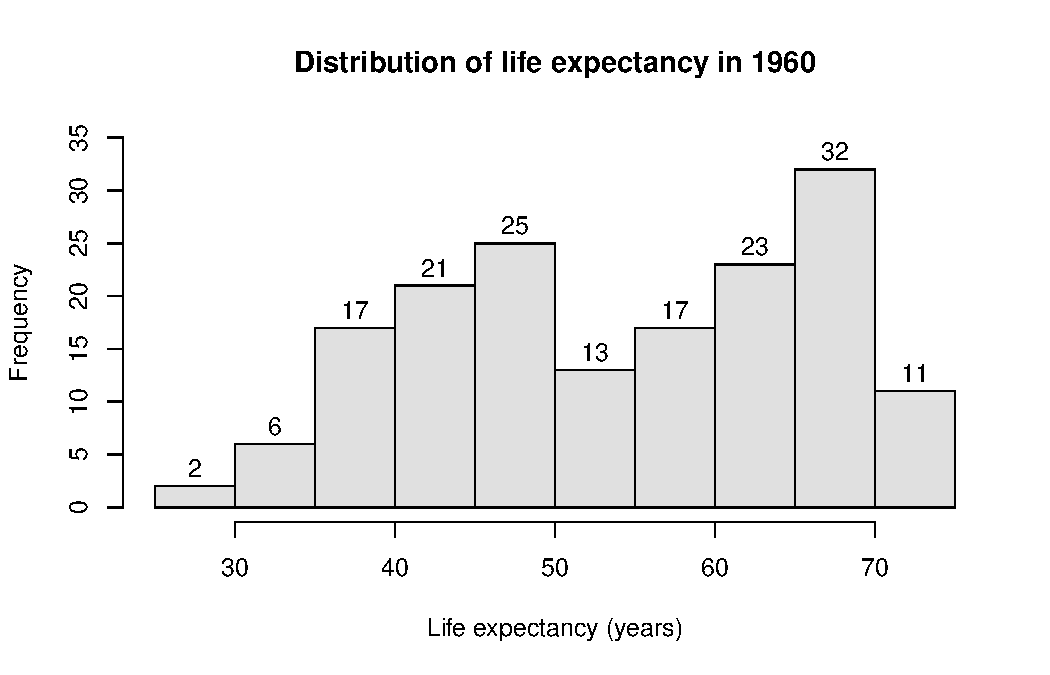
\includegraphics[width=\maxwidth]{week8/week8-sol1-1} 

\end{knitrout}
\end{minipage}
\begin{minipage}{.45\textwidth}
\begin{knitrout}\footnotesize
\definecolor{shadecolor}{rgb}{0.969, 0.969, 0.969}\color{fgcolor}
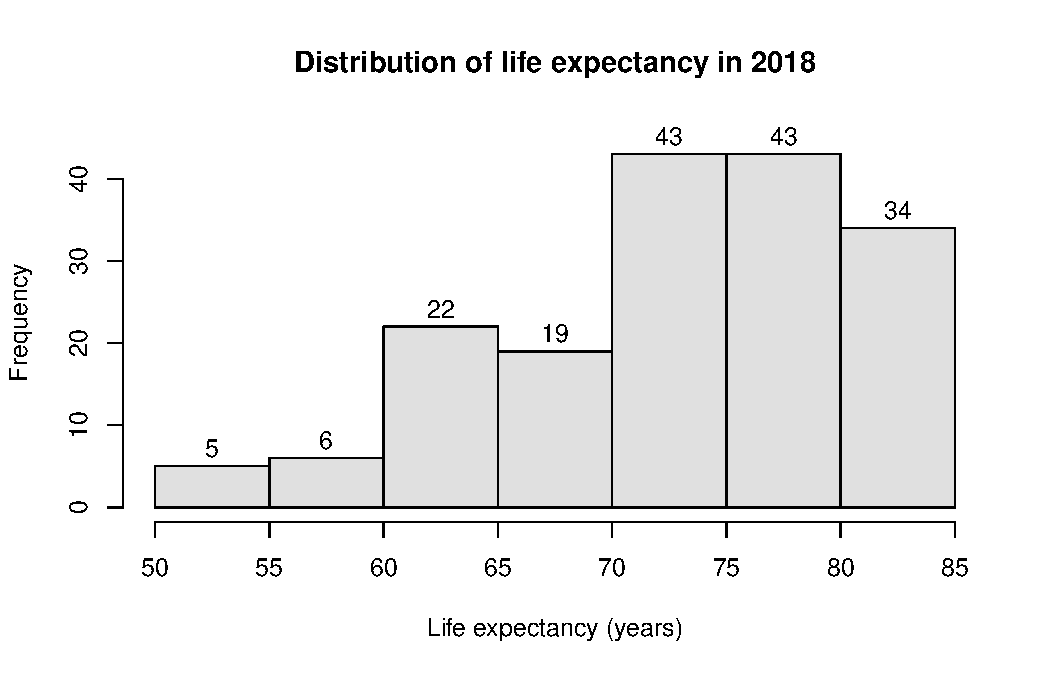
\includegraphics[width=\maxwidth]{week8/week8-sol2-1} 

\end{knitrout}
\end{minipage}
\end{center}

\subsubsection*{Question 2}
\begin{enumerate}[a)]
\item The proportions are the area of the rectangles. The height of
  the bar associated with the interval 8.5 to 9.0 is 0.289 and its
  base is 0.5, so the area is 0.289$\times$0.5 = 0.1445. Therefore
  14.45\% of the countries are located in that interval. Since the
  total number of countries is 180, the number of countries in the
  interval is 0.1445$\times$180 = 26.

\item The density times the interval length is the proportion. The
  proportion of countries with a real per capital GDP between 0 and 5
  thousand dollars is 78/180 = 0.4333. The density value is therefore
  the proportion divided by the interval length: 0.4333/5 = 0.087. The
  main difference between the a) and b) histograms is that the one in
  b) is skewed to the right while the one in a) is not skewed.


\item The difference between the third and first quintiles is
  5.25 thousand dollars and the difference between the fifth
  quintile and the third is 23.81 thousand dollars. Therefore,
  the tail is must longer on the right of the third quintile (which is
  the center). Using the variable expressed in logs, the difference
  between the third and first quintiles is 1.74 and the
  difference between the fifth quintile and the third is
  1.5. Therefore, there is little difference between the length
  of the tail on the right and left sides of the third quintile. The
  reason is that differences in proportion is almost equal and
  differences in dollars are very different: If $X_i$ is the average
  per capita GDP for the i$^\mathrm{th}$ quintile, then:
\begin{eqnarray*}
\log(X_3)-\log(X_1) &=& \log\left(\frac{X_3}{X_1}\right) =
1.74\\ \frac{X_3}{X_1} & = & e^{1.74} =
5.7
\end{eqnarray*}
and
\begin{eqnarray*}
\log(X_5)-\log(X_3) &=& \log\left(\frac{X_5}{X_3}\right) =
1.5\\ \frac{X_5}{X_3} & = & e^{1.5} =
4.48
\end{eqnarray*}
Therefore, the average real per capita GDP for the third quintile is
5.7 time the one for the first quintile and the
average real per capita GDP for the fifth quintile is
4.48 times the one for the third quintile. The
difference is not as high as the difference in dollars. 

Think about it, the average income in the first quintile is
1.14 thousand. Therefore, 5.7 times
1.14 thousand means a difference of
5.358 thousand
([5.7 $\times$
  1.14]-1.14). On the other hand, the average
income in the third quintile is 6.39 thousand. Therefore,
4.48 times 6.39 thousand means a
difference of 22.2372 thousand. 

\end{enumerate}
\subsubsection*{Question 3}

\begin{enumerate}[a)]
\item The two initially poorest countries are Portugal
  (PRT) and Cyprus (CYP) and the
  two intially richest countries are Sweden
  (SWE) and Luxembourg (LUX). On the
  following chart, they are represented respectively by the solid
  black, the dashed red, the dotted green and the dot-dashed blue
  lines. No country is converging to the country that was initially
  the richest (LUX). Cyprus is getting closer to Sweden (it is
  converging slowly) but the gap between Portugal and Sweden has not
  changed much over the period (no convergence).
  \begin{center}

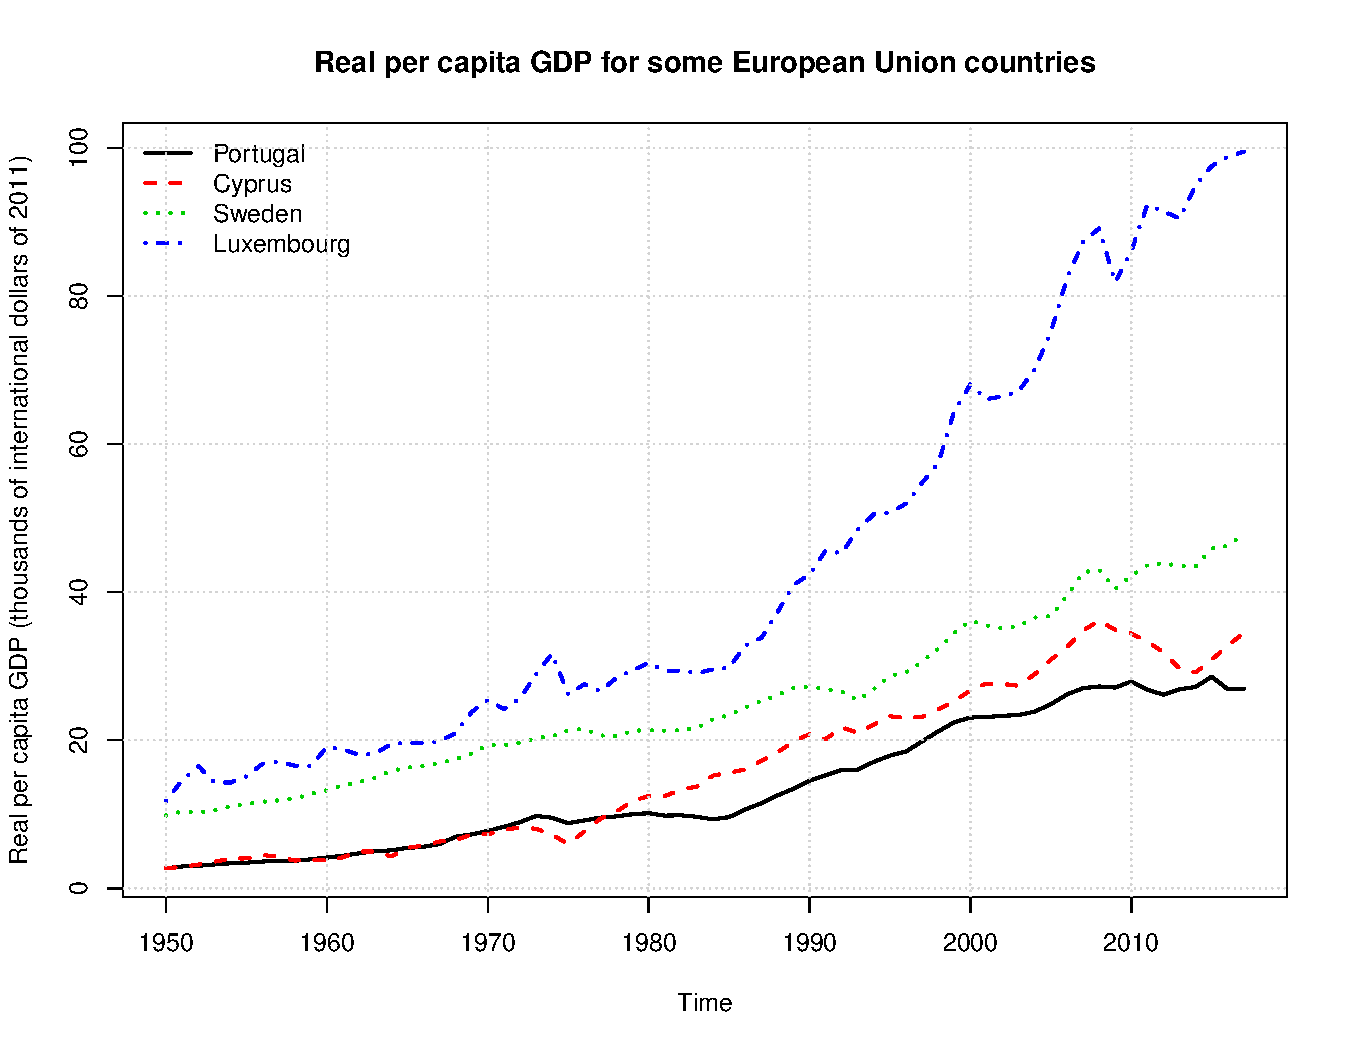
\includegraphics[width=0.6\linewidth]{week8/week8-sol3-1} 

\end{center}    
\item The same line shapes and colors are used for the four countries
  in the following chart. The chart tells a similar story, but the
  gaps are now proportions which makes it a little harder to
  interpret.
\begin{center}

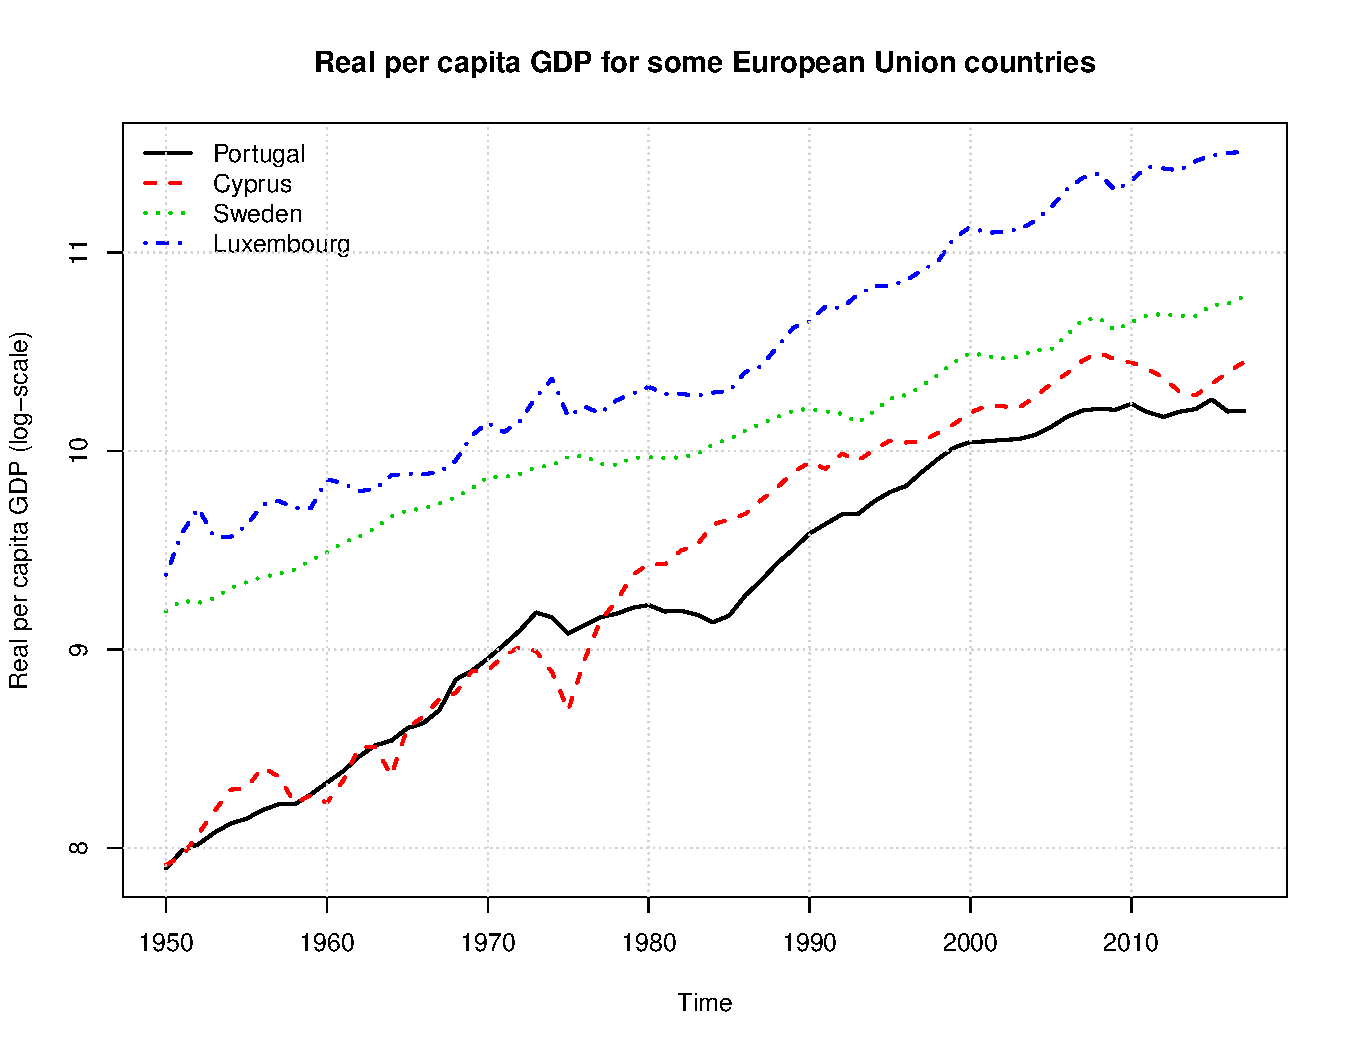
\includegraphics[width=0.6\linewidth]{week8/week8-sol4-1} 

\end{center}    
If we compare Luxembourg and Sweden, we clearly see that gap increased
in proportion. This is consistent with the huge increase in the gap in
dollars that we see on the previous answer. Always remember that if
gap=$\log(X_2)-\log(X_1)$, where in this case $X_2$ and $X_1$ are
respectively the real per capita GDP of Luxembourg and Sweden in
thousands of dollars, then
\[
X_2 = X_1 e^{\mathrm{gap}}\,,
\]
which implies the following difference (subtract $X_1$ on both sides):
\[
X_2-X_1 = X_1 \left(e^{\mathrm{gap}}-1\right)\,.
\]
Therefore, if the difference in logs is constant (same gap) but $X_1$
is increasing (Sweden is growing), then the gap in dollars is
increasing. If we compare Portugal and Sweden, the gap in logs is
decreasing over the period (the lines are getting closer to each
other) but it is constant in dollars. What happens is that the
increase in $X_1$ is offset by the smaller gap, so that the difference
in dollars remains constant. 
\item The following is the scatter plot on which the country codes
  have been added. If we ignore Ireland (IRL) and Luxembourg (LUX) we
  almost get a perfect negative comovement between the two
  variables. Therefore, we observe convergence among EU countries.
\begin{center}

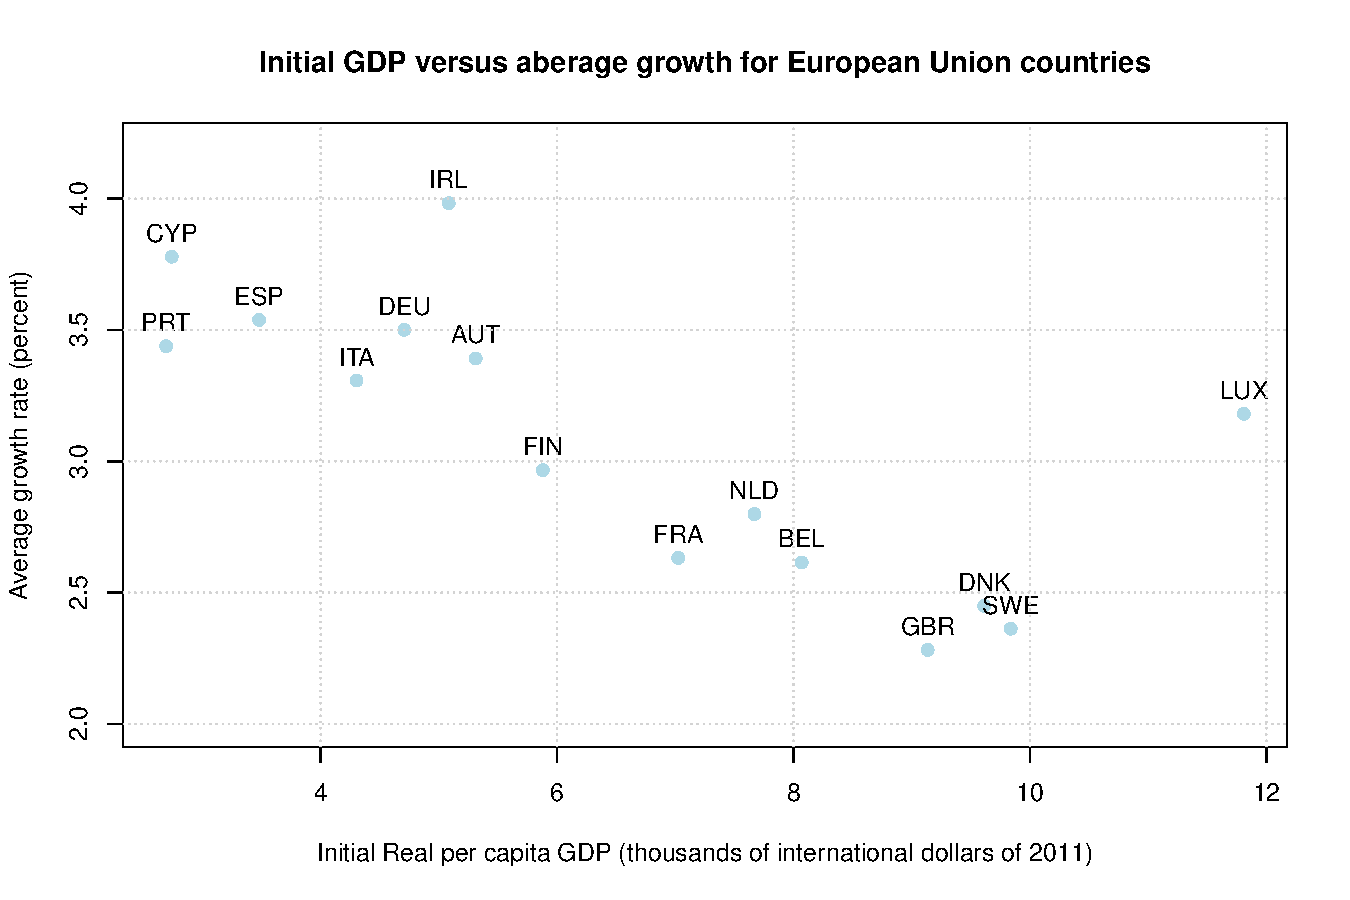
\includegraphics[width=0.6\linewidth]{week8/week8-sol5-1} 

\end{center}
\item The following are the characteristics found in the
  Characteristics.csv file for Ireland and Italy:
\begin{center}  
\resizebox{0.8\linewidth}{!}{    
% latex table generated in R 3.6.3 by xtable 1.8-4 package
% Fri May 15 16:13:02 2020
\begin{tabular}{rrrrrrr}
  \hline
 & GovShare & InvShare & Openness & Life & Education & Literacy \\ 
  \hline
Ireland & 15.03 & 24.43 & 95.27 & 75.10 & 61.19 & 99.00 \\ 
  Italy & 14.87 & 26.48 & 38.14 & 76.51 & 41.77 & 98.22 \\ 
   \hline
\end{tabular}

}
\end{center}
All characteristics are similar except for the education and level of
openness which are much higher for Ireland. We saw in the chapter that
countries with higher level of openness and larger proportion of
adults with at least an upper secondary degree tend to grow faster on
average. Therefore, the higher education and level of openness could
explain why Ireland grew faster than Italy. Am I certain that
education and openness explain the difference? The answer is
no. First, we saw lots of variation in the scatter plots of growth
versus characteristics: many countries with lower level of openness
and education grow faster. Also, comovements do not imply direct
relationships. It is just a possibility that needs to be justified by
theory.
\end{enumerate}

\subsubsection*{Question 4}

\begin{enumerate}[a)]
\item The two initially poorest countries are Mali
  (MLI) and Burkina Faso (BFA) and the two
  intially richest countries are Senegal (SEN)
  and Ghana (GHA). On the following chart, they
  are represented respectively by the solid black, the dashed red, the
  dotted green and the dot-dashed blue lines, and Cabo Verde is the
  long-dashed cyan line. First, not only Cabo Verde converged to the
  initially richest countries, it became the richest. It is clearly
  the country with the highest growth rate. The Senegal and Ghana did
  not grow much during the period. In fact, it took 60 years for them
  to see their real per capita GDP's exceed their 1950 level. As a
  result, the initially poorest countries are converging to Senegal
  and Ghana despite their small (but positive) growth rate.
  \begin{center}

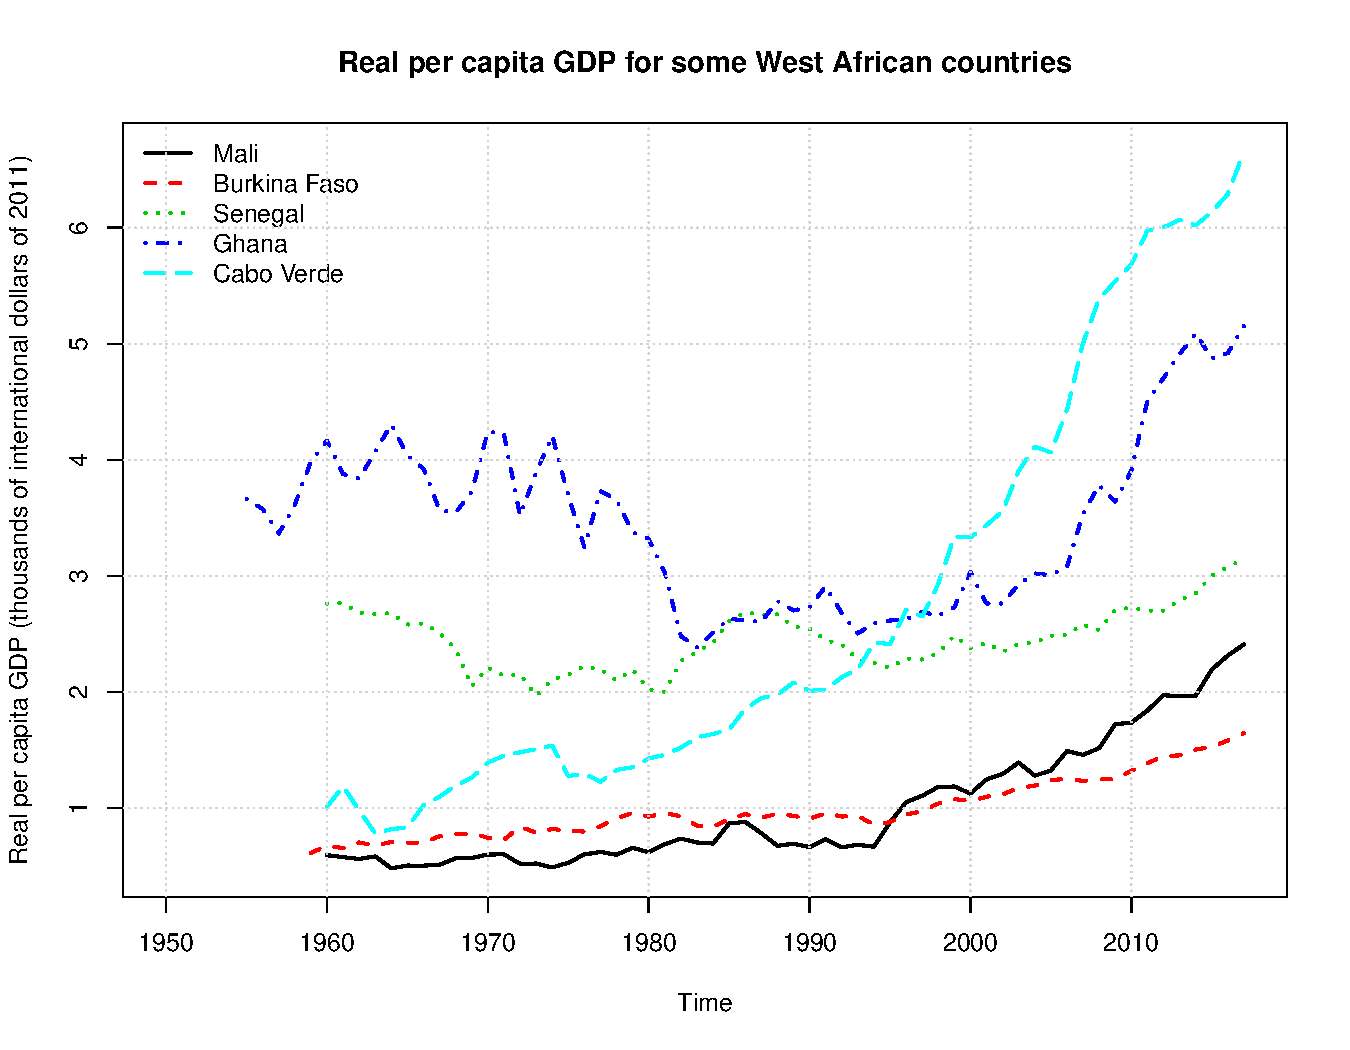
\includegraphics[width=0.6\linewidth]{week8/week8-sol6-1} 

\end{center}    
\item The same line shapes and colors are used for the five countries
  in the following chart. The chart tells a similar story. Notice that
  from 2000, Cabo Verde, Ghana and Mali are growing at the same rate
  (the lines are parallel and we use the log-scale). But since they
  are different real per capita GDP, the gaps in dollars are
  increasing.
\begin{center}

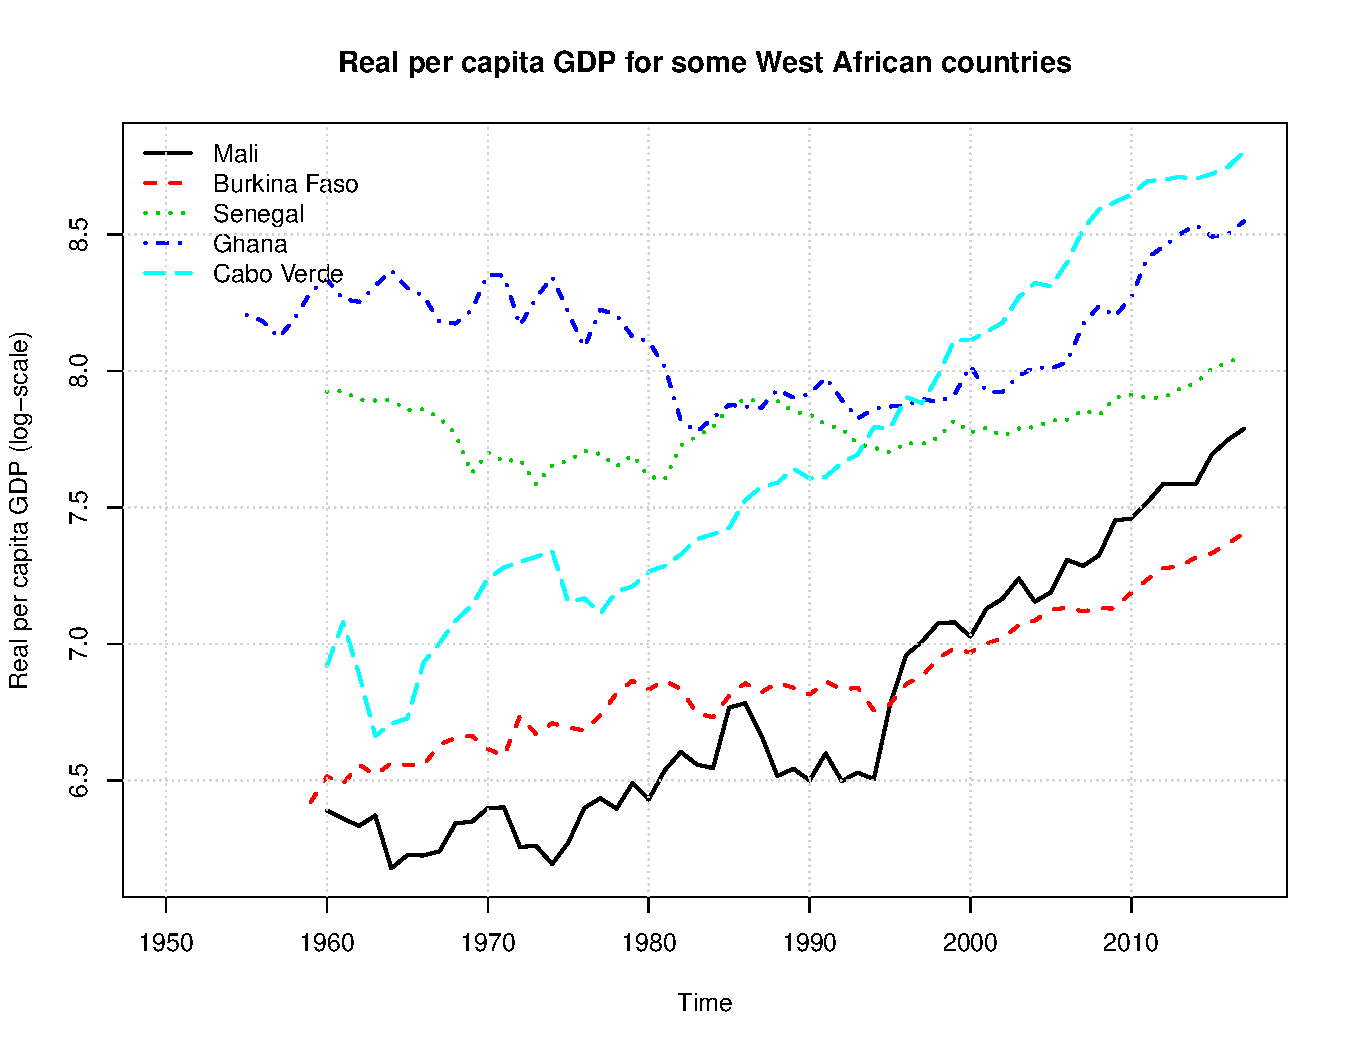
\includegraphics[width=0.6\linewidth]{week8/week8-sol7-1} 

\end{center}    

\item The following is the scatter plot on which the country codes
  have been added. We observe a negative comovement, which implies
  convergence, but there are much more variation compared with the EU
  countries. Therefore, many countries that were poor in the '50s are
  still poor today (four countries have an average growth rate less
  than 0).
\begin{center}

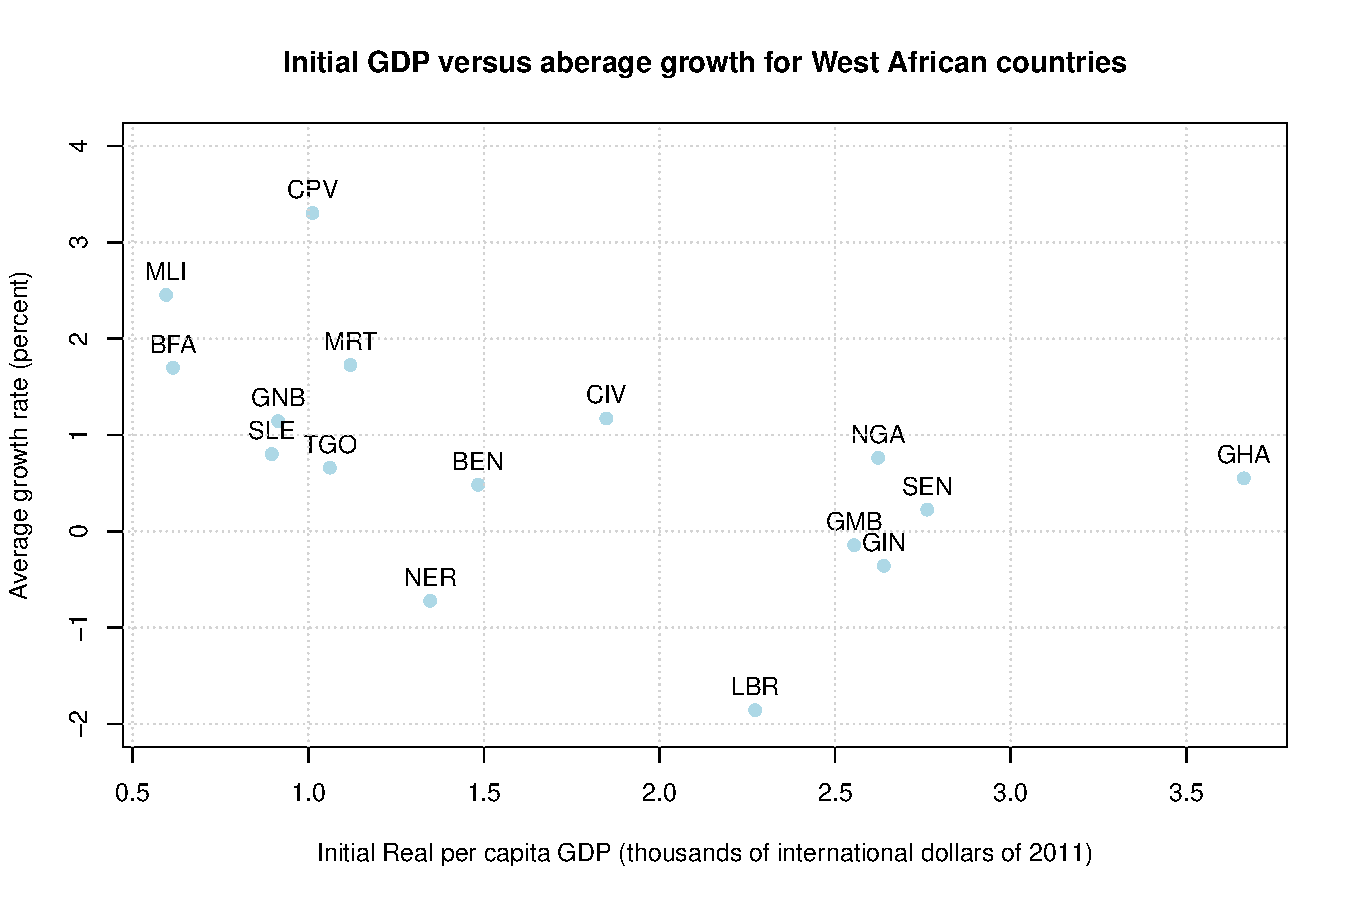
\includegraphics[width=0.6\linewidth]{week8/week8-sol8-1} 

\end{center}
\item The following are the characteristics found in the
  Characteristics.csv and EconFreedom.csv for Cabo Verde, Guinea and
  Niger. For the economic freedom index, we report the average over
  the available period.
\begin{center}  
\resizebox{0.8\linewidth}{!}{    
% latex table generated in R 3.6.3 by xtable 1.8-4 package
% Fri May 15 16:13:02 2020
\begin{tabular}{rrrrrrrrr}
  \hline
 & Growth & GovShare & InvShare & Openness & Life & Education & Literacy & EconFreedom \\ 
  \hline
Cabo Verde & 3.30 & 15.97 & 49.07 & 41.30 & 62.93 & 20.04 & 77.76 & 6.87 \\ 
  Guinea & -0.36 & 10.17 & 8.20 & 22.47 & 46.92 & 6.74 & 26.89 & 5.58 \\ 
  Niger & -0.72 & 22.83 & 20.05 & 17.83 & 45.21 & 3.28 & 24.54 & 5.23 \\ 
   \hline
\end{tabular}

}
\end{center}
We will ignore differences in the government spending share because we
have not observed a strong comovement between this variable and the
growth rate in the chapter. If we compare Cabo Verde with the other two
countries, there is a clear difference. Investment share is 5 times
the share in Guinea and more than twice the share in Niger. Also,
there are at least 3 times more individuals with at least an upper
secondary education in Capo Verde and the literacy rate is also 3
times higher. There is also a large difference for the Economic
freedom index, the level of openness and life expectancy. For the
economic freedom, it is hard to interpret what it means to have a
difference of 1.3. Let's say, given that it is 8.08 in Canada, that
Capo Verde is between Guinea and Canada. With these huge differences,
we can say that all of these differences have something to do with the
relative success of Cabo Verde. However, we need the theory to explain
why they might affect growth and what are their relative importance.

For Niger and Guinea, they have similar characteristics. The
investment is higher in Guinea but the openness and education are
lower.
\end{enumerate}

\subsubsection*{Question 5}
\begin{enumerate}[a)]
\item You can answer the question in two ways. First, you calculate
  the final real per capita GDP for each countries:
\[
X_A = 5\times(1.01)^{60} = 9.08
\]
\[
X_B = 5\times(1.02)^{60} = 16.41
\]
Which implies:
\[
\frac{X_B}{X_A} = 1.81\,.
\]
You can also calculate it directly:
\[
\frac{X_B}{X_A} = \frac{5\times (1.02)^{60}}{5\times (1.01)^{60}}
= \frac{(1.02)^{60}}{(1.01)^{60}} = \left(\frac{1.02}{1.01}\right)^{60}
=1.81
\]
It means that real per capita GDP in country B is
1.81 times higher than in country A after
60 years.
\item Since the real per capita GDP doubles, $X_t/X_0=2$. Therefore:
\[
2 = (1+g)^t  
\]
Knowing $g$, we solve for $t$. For country A, we have:
\begin{eqnarray*}
2 &=& 1.01^t\\
\log(2) &=& t\log(1.01) \\
\frac{\log(2)}{\log(1.01)} &=& t\\
69.7 &=& t
\end{eqnarray*}
Similarly, we have the following for country B:
\[
t = \frac{\log(2)}{\log(1.02)}  = 35
\]
Therefore, it takes 35 years for
country B to double its real per capita GDP and
69.7 years for country A.
\item We are looking for $t$ that will make the final values of two
  countries equal. For countries A and C, we need to solve the
  following equation:
\[
10\times(1.03)^t = 50\times(1.015)^t
\]
Using the properties of logarithm, we obtain:
\begin{eqnarray*}
\log(10) + t \log(1.03) &=& \log(50)+t\log(1.015)\\
 t [\log(1.03)-\log(1.015)] &=& [\log(50)-\log(10)]\\
 t &=& \frac{\log(50)-\log(10)}{\log(1.03)-\log(1.015)}\\
 t &=&109.7
\end{eqnarray*}
Similarly \, we obtain the following for country B:
\begin{eqnarray*}
 t &=& \frac{\log(50)-\log(10)}{\log(1.04)-\log(1.015)}\\
 t &=&66.1
\end{eqnarray*}
Therefore, it will take
109.7 years for
country A to converge to country C and it will take
66.1 years for
country B.
\item We can apply the same formula used in the previous solution. You
  just need to plug the numbers from the table in it. The following shows the results:
\begin{center}
\resizebox{0.9\linewidth}{!}{      
% latex table generated in R 3.6.3 by xtable 1.8-4 package
% Fri May 15 16:13:02 2020
\begin{tabular}{ccccc}
  \hline
 & Annual growth rate (percent) & real per capita GDP in 2017 (thousands of dollars) & Number of Years & Year of convergence \\ 
  \hline
Canada & 2.06 & 44.49 &  &  \\ 
  Nepal & 2.21 & 2.45 & 1974 & 3991 \\ 
  Hungary & 3.41 & 27.53 &  37 & 2054 \\ 
  Greece & 3.06 & 25.38 &  58 & 2075 \\ 
  Lao People's DR & 4.88 & 6.56 &  70 & 2087 \\ 
   \hline
\end{tabular}

}
\end{center}  
The third column is the number of years to converge to Canada (rounded
to the nearest integer) and the last of the year when the country will
have reached the real per capita GDP of Canada (2017+number of
years). For example, it will take 1974 years for
Nepal to converge to Canada. Therefore, it will
happen in the year 3991. 
\item It is probably not reasonable. Even if some poor countries have
  not grown over the period, countries with favorable characteristics
  (high education, investment share, health) tend to grow at a slower
  rate on average as they get richer (conditional
  convergence). Therefore, it is not reasonable to assume that growth
  rate will remain constant as real per capita GDP increases.

\end{enumerate}

\bibliography{econ102}
\end{document}
